\documentclass{article}

\title{\huge {Hyena Hierarchy:}\\Towards Larger Convolutional Language Models}
%
%
 \author{Michael Poli\footnote{Equal contribution. $\dagger$ Equal senior authorship. $^1$Stanford University. $^2$Mila and Universit\'e de Montr\'eal.}~$^{,1}$, Stefano Massaroli$^{*,2}$, Eric Nguyen$^{1,*}$, \\ Daniel Y. Fu$^1$, Tri Dao$^1$, Stephen Baccus$^1$, \\ Yoshua Bengio$^2$, Stefano Ermon$^{1,\dagger}$, Christopher R\'e$^{1,\dagger}$
 }
 
\date{\small{\footnotesize\sf Version}: submitted draft, {\footnotesize\sf  Last Compiled}: \today}
%
% \newcommand{\ourmethod}{{\tt S4caster}}
\newcommand{\ourmethod}{\textsc{SpaceTime}}
\newcommand{\ourmethodunit}{\textsc{SpaceTime} layer}
\newcommand{\numberMonashTasks}{34}  % {58}
\newcommand{\numberInformerTasks}{16}

% Style to highlight edits, comments, todos, suggestions
\newcommand{\working}[1]{\textcolor{purple}{\authnote{}{#1}}}
\newcommand{\MZ}[1]{\textcolor{cyan}{\authnote{(MZ: }{#1})}}
\newcommand{\KS}[1]{\textcolor{orange}{\authnote{(KS: }{#1})}}
\newcommand{\tempcite}[1]{\textcolor{red}{(cite)}}

% Additional header / formatting
\newcommand{\header}[1]{\textbf{#1.}}
\newcommand{\subheader}[1]{\textbf{\textit{#1.}}}
\usepackage{enumitem}  % margins in lists

\usepackage{minitoc,wrapfig}
\renewcommand \thepart{}
\renewcommand \partname{}

% Other text abbreviations
\makeatletter
\DeclareRobustCommand\onedot{\futurelet\@let@token\@onedot}
\def\@onedot{\ifx\@let@token.\else.\null\fi\xspace}

\def\eg{\emph{e.g.},} 
\def\Eg{\emph{E.g.},}
\def\ie{\emph{i.e.},} 
\def\Ie{\emph{I.e.},}
\def\cf{\emph{c.f.},} 
\def\Cf{\emph{C.f.},}
\def\st{\emph{s.t}\onedot}
\def\etc{\emph{etc}\onedot} 
\def\vs{\emph{vs}\onedot}
\def\wrt{w.r.t.} 
\def\dof{d.o.f\onedot}
\def\iid{i.i.d\onedot} 
\def\wolog{w.l.o.g\onedot}
\def\etal{\emph{et al}\onedot}

% tikz
% colors and graphics
\usepackage{graphicx}
\usepackage{tikz}
\usepackage{tikz-cd}
\usepackage{hf-tikz}
\usepackage{pgfplots} 
\pgfplotsset{compat=1.17} 
\pgfplotsset{
        table/search path={figures/drawings},
    }
\usepackage{rotating}
\usetikzlibrary{fadings}
\usetikzlibrary{shapes, arrows, fit, backgrounds, arrows.meta}

\usetikzlibrary{matrix}
\usetikzlibrary{shadows.blur}
\usetikzlibrary{patterns, tikzmark}
\usetikzlibrary{decorations.pathreplacing, calc, decorations.markings,}

% Tables
\usepackage{adjustbox}
\usepackage{varwidth}

%% Tables
\usepackage{booktabs}
\usepackage{multirow}
\usepackage[normalem]{ulem}
\useunder{\uline}{\ul}{}
%% Table colors
\usepackage{colortbl} 
\definecolor{Gray}{gray}{0.90}  
% 0.85
\definecolor{LightCyan}{rgb}{0.7,1,1}
\definecolor{White}{rgb}{1,1,1}
\newcolumntype{a}{>{\columncolor{Gray}}c}
\newcolumntype{b}{>{\columncolor{LightCyan}}c}
\newcolumntype{n}{>{\columncolor{White}}c}
% \usepackage[table,xcdraw]{xcolor}
\usepackage{rotating}



\newcommand{\fcircle}[2][red,fill=red]{\tikz[baseline=-0.5ex]\draw[#1,radius=#2] (0,0.03) circle ;}


% Algorithms
\usepackage{algorithm}
\usepackage{algpseudocode}

% Figures
% \usepackage{subfig}

% Checkmark and Xmark
\newcommand{\cmark}{\ding{51}}%
\newcommand{\xmark}{\ding{55}}%
\usepackage{amsmath, amssymb, amsfonts, mathtools}
\usepackage{physics}
\usepackage{cancel}
\usepackage{thmtools, thm-restate}
\usepackage{accents}

% COMMANDS
\DeclareMathOperator{\st}{subject~to}
\DeclareMathOperator{\Span}{span}
\DeclareMathOperator{\vect}{vec}
\DeclareMathOperator{\diag}{diag}
\DeclareMathOperator*{\topk}{top}
\DeclareMathOperator{\rad}{rad}
\DeclareMathOperator{\argmin}{arg min}
\DeclareMathOperator{\dom}{dom}
\newcommand{\x}{\times}
\newcommand{\ubar}[1]{\underaccent{\bar}{#1}}
\newcommand{\inner}[3][]{\ensuremath{\left\langle #2, \, #3 \right\rangle_{#1}}}

\usepackage{pict2e, picture}
\makeatletter
\DeclareRobustCommand{\Arrow}[1][]{%
\check@mathfonts
\if\relax\detokenize{#1}\relax
\settowidth{\dimen@}{$\m@th\rightarrow$}%
\else
\setlength{\dimen@}{#1}%
\fi
\sbox\z@{\usefont{U}{lasy}{m}{n}\symbol{41}}%
\begin{picture}(\dimen@,\ht\z@)
\roundcap
\put(\dimexpr\dimen@-.7\wd\z@,0){\usebox\z@}
\put(0,\fontdimen22\textfont2){\line(1,0){\dimen@}}
\end{picture}%
}
\makeatother
\newcommand{\shortarrow}{\vspace*{1mm}\hspace{.2mm}\scalebox{.8}{\Arrow[.1cm]}\hspace{.2mm}}

\newcommand{\cB}{\mathcal{B}}
\newcommand{\cC}{\mathcal{C}}
\newcommand{\cD}{\mathcal{D}}
\newcommand{\cE}{\mathcal{E}}
\newcommand{\cL}{\mathcal{L}}
\newcommand{\cN}{\mathcal{N}}
\newcommand{\cO}{\mathcal{O}}
\newcommand{\cT}{\mathcal{T}}
\newcommand{\cU}{\mathcal{U}}
\newcommand{\cX}{\mathcal{X}}
\newcommand{\cF}{\mathcal{F}}
\newcommand{\cG}{\mathcal{G}}
\newcommand{\cQ}{\mathcal{Q}}
\newcommand{\cR}{\mathcal{R}}
\newcommand{\cV}{\mathcal{V}}
\newcommand{\cW}{\mathcal{W}}
\newcommand{\cY}{\mathcal{Y}}
\newcommand{\cZ}{\mathcal{Z}}

\newcommand{\zb}{\mathbf{z}}
\newcommand{\xb}{\mathbf{x}}

\newcommand{\sA}{\mathsf{A}}
\newcommand{\sB}{\mathsf{B}}
\newcommand{\sC}{\mathsf{C}}
\newcommand{\sD}{\mathsf{D}}
\newcommand{\sE}{\mathsf{E}}
\newcommand{\sF}{\mathsf{F}}
\newcommand{\sG}{\mathsf{G}}
\newcommand{\sH}{\mathsf{H}}
\newcommand{\sI}{\mathsf{I}}
\newcommand{\sL}{\mathsf{L}}
\newcommand{\sM}{\mathsf{M}}
\newcommand{\sN}{\mathsf{N}}
\newcommand{\sO}{\mathsf{O}}
\newcommand{\sP}{\mathsf{P}}
\newcommand{\sQ}{\mathsf{Q}}
\newcommand{\sR}{\mathsf{R}}
\newcommand{\sS}{\mathsf{S}}
\newcommand{\sT}{\mathsf{T}}
\newcommand{\sU}{\mathsf{U}}
\newcommand{\sW}{\mathsf{W}}
\newcommand{\sX}{\mathsf{X}}
\newcommand{\sY}{\mathsf{Y}}
\newcommand{\sZ}{\mathsf{Z}}
\newcommand{\sg}{\mathsf{g}}

\newcommand{\nA}{{n_a}}
\newcommand{\nU}{{n_u}}
\newcommand{\nX}{{n_x}}
\newcommand{\nZ}{{n_z}}
\newcommand{\nW}{{n_w}}
\newcommand{\nT}{{n_\theta}}
\newcommand{\nN}{{n_\xi}}
\newcommand{\nQ}{{n_q}}

\newcommand{\la}{\left\langle}
\newcommand{\ra}{\right\rangle}
\newcommand{\lb}{\left[}
\newcommand{\rb}{\right]}
\newcommand{\lc}{\left(}
\newcommand{\rc}{\right)}

\newcommand{\bA}{\mathbb{A}}
\newcommand{\bB}{\mathbb{B}}
\newcommand{\bC}{\mathbb{C}}
\newcommand{\bD}{\mathbb{D}}
\newcommand{\bE}{\mathbb{E}}
\newcommand{\bF}{\mathbb{F}}
\newcommand{\bG}{\mathbb{G}}
\newcommand{\bH}{\mathbb{H}}
\newcommand{\bI}{\mathbb{I}}
\newcommand{\Id}{\mathbb{I}}
\newcommand{\bK}{\mathbb{K}}
\newcommand{\bL}{\mathbb{L}}
\newcommand{\bM}{\mathbb{M}}
\newcommand{\bN}{\mathbb{N}}
\newcommand{\bO}{\mathbb{O}}
\newcommand{\bP}{\mathbb{P}}
\newcommand{\bQ}{\mathbb{Q}}
\newcommand{\R}{\mathbb{R}}
\newcommand{\bS}{\mathbb{S}}
\newcommand{\bT}{\mathbb{T}}
\newcommand{\bU}{\mathbb{U}}
\newcommand{\bV}{\mathbb{V}}
\newcommand{\bW}{\mathbb{W}}
\newcommand{\bX}{\mathbb{X}}
\newcommand{\bY}{\mathbb{Y}}
\newcommand{\bZ}{\mathbb{Z}}


\DeclareMathAlphabet{\nummathbb}{U}{BOONDOX-ds}{m}{n}
\newcommand{\0}{\nummathbb{0}}
\newcommand{\Oz}{\nummathbb{O}}
\newcommand{\1}{\nummathbb{1}}

\newcommand{\eps}{\epsilon}

\makeatletter
\DeclareRobustCommand\widecheck[1]{{\mathpalette\@widecheck{#1}}}
\def\@widecheck#1#2{%
    \setbox\z@\hbox{\m@th$#1#2$}%
    \setbox\tw@\hbox{\m@th$#1%
       \widehat{%
          \vrule\@width\z@\@height\ht\z@
          \vrule\@height\z@\@width\wd\z@}$}%
    \dp\tw@-\ht\z@
    \@tempdima\ht\z@ \advance\@tempdima2\ht\tw@ \divide\@tempdima\thr@@
    \setbox\tw@\hbox{%
       \raise\@tempdima\hbox{\scalebox{1}[-1]{\lower\@tempdima\box
\tw@}}}%
    {\ooalign{\box\tw@ \cr \box\z@}}}
\makeatother


\begin{document}
\maketitle
%
 \begin{abstract}
    Recent advances in deep learning have relied heavily on the use of large Transformers due to their ability to learn at scale. However, the core building block of Transformers, the attention operator, exhibits quadratic cost in sequence length, limiting the amount of context accessible. Existing subquadratic methods based on low-rank and sparse approximations need to be combined with dense attention layers to match Transformers, indicating a gap in capability. In this work, we propose \textbf{Hyena}, a subquadratic drop-in replacement for attention constructed by interleaving implicitly parametrized \textbf{long convolutions} and \textbf{data-controlled gating}. In recall and reasoning tasks on sequences of thousands to hundreds of thousands of tokens, Hyena improves accuracy by more than $50$ points over operators relying on state-spaces and other implicit and explicit methods, matching attention-based models. We set a new state-of-the-art for dense-attention-free architectures on language modeling in standard datasets ({\sc WikiText103} and {\sc The Pile}), reaching Transformer quality with a $20\%$ reduction in training compute required at sequence length $2$K. Hyena operators are twice as fast as highly optimized attention at sequence length $8$K, and $100\x$ faster at sequence length $64$K.
\end{abstract}
%

\setlength\abovedisplayshortskip{2pt}
\setlength\belowdisplayshortskip{2pt}
\setlength\abovedisplayskip{2pt}
\setlength\belowdisplayskip{2pt}

% % % content here
\section{Introduction}
Reinforcement Learning from Human Feedback (RLHF) is a technique that can be used to align an agent --- such as a Large Language Model (LLM) --- to human preferences and lead to more truthful, more helpful, less harmful and more preferred outputs \cite{ouyang2022training}. Proximal Policy Optimization (PPO) \cite{schulman2017proximal} and Direct Preference Optimization (DPO) \cite{rafailov2023direct} are two such aligment techniques which have been extensively used to improve the quality of LLM outputs, leading to instruction following agents or chat assistants which are quickly approaching human-baselines in a variety of knowledge and reasoning tasks \cite{open-llm-leaderboard, clark2018think, zellers2019hellaswag, hendrycks2021measuring, lin2022truthfulqa, DBLP:journals/corr/abs-1907-10641, DBLP:journals/corr/abs-2110-14168}.

However, recent research has shown that RLHF may actually hurt an LLM's reasoning abilities rather than improving it. One study \cite{bekbayev2023poison} discovered that performing alignment during the Supervised Fine-Tuning (SFT) stage of training may lead to worse performance on reasoning benchmarks, and another \cite{bai2022training} discovered that SFT alone outperforms RLHF for smaller models with the benefits of RLHF only emerging for models with more than 1 Billion parameters. Ouyang et al. \cite{ouyang2022training} also reports an increased tendency for RLHF models to make up information in closed domain tasks (``hallucination'') compared to models trained with SFT alone.

To combat the the risk of RLHF compromising the abilities of an LLM in favor of producing preferable outputs we introduce Direct Preference Heads (DPH), a novel feature based approach that optimises a reward score produced by the LLM rather than optimising the logits produced by language modelling head. DPH can be used in combination with (or without) existing alignment techniques to allow language models to self-evaluate outputs sampled at inference time and select the highest scoring candidate.

We evaluate the performance of DPH using an efficient 551M parameter LM on a variety of commonsense reasoning and Natural Language Understanding (NLU) tasks. All code used to train our models is available on \anon{\href{https://github.com/Avelina9X/direct-preference-heads}{GitHub}} and we release our model weights on \anon{\href{https://huggingface.co/collections/Avelina/direct-preference-heads-preprint-6612d8a6fa3843352943fd43}{Hugging Face}}.
\section{Preliminaries and Related Work}\label{back}
% 
A discrete convolution is a function of two arguments: an input $u$ signal of length $L$ and a learnable filter $h$. The linear (aperiodic) convolution of a (possibly infinitely long) measurable\footnote{In the $L^1(\bZ)$ sense: $\sum_{t=-\infty}^\infty |h_t|<\infty$} filter $h$ with a length-$L$ input signal $u$ is defined as
%
\begin{equation}\label{eq:cnn}
    \begin{aligned} 
        y_t = (h * u)_t = \sum_{n=0}^{L-1} h_{t -n} u_n.
    \end{aligned}
\end{equation}
%

Generally, $u_t\in\R^D$ where $D$ is the width of the signal, or in deep learning parlance, the number of \textit{channels}. Without loss of generality, we specialize our analysis to \textit{single input single output} (SISO) layers, i.e. with $D=1$. The \textit{multiple input multiple output} (MIMO) case, canonical in standard convolutional layers, follows directly.
%

In this case, the input signal can be represented as a vector $u\in\R^L$ and the convolution as a matrix-vector product between the input and the Toeplitz kernel matrix $\sS_h \in \R^{L \times L}$ induced by the filter $h$:
%
\begin{equation}\label{eq:cnn_matvec}
    \begin{aligned} 
        %
        (h * u) = 
        %
        \begin{bmatrix}
            h_0 & h_{-1} & \cdots & h_{-L+1} \\
            h_1 & h_0 & \cdots & h_{-L+2} \\
            \vdots & \vdots & \ddots & \vdots \\
            h_{L-1} & h_{L-2} & \cdots & h_{0}
        \end{bmatrix}
        \begin{bmatrix}
            u_0\\
            u_1\\
            \vdots\\
            u_{L-1}
        \end{bmatrix}
    \end{aligned}
\end{equation}
%
\subsection{Explicit and Implicit Convolutions}
%
Parametrizing and optimizing convolution filters $h_t$ is a standard procedure in deep learning and more broadly signal processing. The classical approach of \textit{convolutional neural networks} (CNNs)  \citep{fukushima1982neocognitron,lecun1998gradient,ronneberger2015u,he2016deep} is to optimize directly the values $h_t$ of the filter's response at $M$ prescribed steps, a parametrization we call \textit{explicit}. $M$ is referred to as the \textit{filter size} and is typically much shorter than the input sequence length $M \ll L$. Such filters are denoted in signal processing as \textit{finite impulse response} (FIR). 

FIR filters are local and can capture dependencies between inputs separated at most by $M$ steps.
Their main advantage is their speed, with complexity $\mathcal{O}(ML)$. However, the number of parameters of FIR filters scales linearly with filter size, which can be computationally prohibitive. To disentangle the parameter count from the filter size, we can instead represent the filter $h_t$ as a parametric function of the time step $t$, i.e. $h_t = \gamma_\theta(t)$, where $\theta$ are the parameters of the function $\gamma_\theta$. This parametrization is called \textit{implicit}. The class of functions $\gamma_\theta$ is a design choice with a significant impact on the expressivity and computational complexity of the layer. 

One choice of implicit parametrization is to select $h$ as the response function of a linear state-space model (SSM) \citep{chen1984linear}, described by the first-order difference equation:
%
\begin{equation*}%\label{eq:ssm}
    %
    \begin{aligned}
        x_{t+1} &= \sA x_t + \sB u_t &&~~ \text{state equation} & \\
        y_t &= \sC x_t + \sD u_t &&~~ \text{output equation} &
    \end{aligned}
    %
\end{equation*}
%
Here, the convenient choice of $x_0 = 0$ renders the input-output map to a simple convolution
%
\[
    \begin{aligned}
        y_t & =\sum_{n=0}^{t}\left(\sC\sA^{t - n}\sB + \sD \delta_{t-n}\right)u_n 
    \end{aligned}
\]
%
where $\delta_t$ denotes the Kronecker delta. We can then identify the filter $h$ as
%
\[
    t\mapsto h_t =
    \begin{cases}
        0 & t<0\\
        \sC \sA^t \sB + \sD\delta_t & t\geq 0
    \end{cases}
\]
%
where the entries of $\sA, \sB, \sC$ and $\sD$ are the learned parameters of the filter. In terms of layer design, the degrees of freedom of SSMs are the dimension of the state and the structure of the matrices. 
SSMs are a canonical example of how long convolutions with sub-linear parameter counts can improve deep learning models for long sequences \citep{gu2020hippo,gu2021efficiently}.
%
 Other implicit approaches include parametrizing filters as maps from (a positional encoding of) $t$ to the filter response i.e.  $\gamma_\theta : t \mapsto h_t=\gamma_\theta(t)$, for example with feed-forward neural networks \citep{romero2021ckconv,romero2021flexconv}. 
%
\begin{tcolorbox}[enhanced, drop fuzzy shadow, frame hidden, sharp corners, breakable, colback=blue!5] \textbf{Long convolutions and memory:} A crude proxy for \textit{memory} of a single computational unit is how far in the past it can access information to produce the output at a certain step. This can be roughly quantified by the number of non-zero entries $\partial y_t / \partial u_{t-n}$ for $n = 0, \ldots, t$. The memory of CNNs filters is equivalent to the filter size $M$ since $\partial y_t / \partial u_{t-n} = h_{n}$. The total mnemonic capacity of an all-convolutions CNN therefore scales with the number of model's parameters. Implicit parametrizations, on the other hand, allow us to disentangle the memory of each filter from the parameter count and where the length of the filter is implicitly controlled by the learned parameters. In an SSM, $\partial y_t / \partial u_{t-n} = \sC \sA^n \sB$ and the memory extent is solely determined by the spectral radius of $\sA$ and can be finely tuned by the training process\footnote{See e.g.\cite{gu2020hippo,gu2021efficiently}}. On the other hand, the number of parameters controls the \textit{expressivity} of the memory unit, e.g. the number of basis functions forming $h_t$. 
\end{tcolorbox}
%
\paragraph{Fast Methods for Convolutions}
%
One of the first applications of the Cooley-Tukey fast Fourier transform (FFT) algorithm was to implement convolution faster than the direct evaluation of \eqref{eq:cnn}.
At first glance \eqref{eq:cnn} comes with $O(L^2)$ an asymptotic time complexity. 
A common approach to achieve \textit{fast long convolutions} in subquadratic time is through the FFT algorithm. The method first converts the \textit{aperiodic} convolution into a \textit{circular} convolution \cite{selesnick2017fast} by appropriate zero-padding of input and filter sequences. The resulting kernel $\hat\sS_h$ is a circulant matrix and is diagonalized by the discrete Fourier basis
%
\[
    \hat \sS_h = \sW^{-1} \sD_{H} \sW
\]
%
where $\sW$ is the DFT matrix, $\sW_{tt'} = z^{-t}, z = e^{i2\pi t'/L}$ and $H$ is the DFT of the padded filter $h$, $H = \sW {\sf pad}(h)$. Thus, the calculation of such convolutions is performed as
%
\begin{equation*}
    \begin{aligned}
        {\sf pad}(y) &= \hat \sS_h {\sf pad}(u) \\
        &= \sW^{-1}\sD_H \sW ~{\sf pad}(u)\\
        &= {\sf iFFT}(\sD_H {\sf FFT}({\sf pad}(u)))
    \end{aligned}
\end{equation*}
%
where $\sD_H$ is the matrix with $\sW h$ on its diagonal. The above is known as the convolution theorem of DFT \citep{oppenheim1997signals}. In this ${\sf FFTConv}$ form the convolution can be performed \textbf{without materializing the operator $\sS_h$} with the same asymptotic cost $O(L\log_2 L)$ of FFT.
%
\subsection{The Self-Attention Operator}
%
At the heart of Transformers is the \textit{multi-head attention} (MHA) mechanism. Given a length-$L$ sequence $u\in\R^{L\times D}$, each \textit{head} of \textit{scaled self-attention} \citep{vaswani2017attention} is a map from $\R^{L\times D}$ to $\R^{L\times D}$ which performs the following operations
%
\begin{equation}\label{eq:att}
    \begin{aligned}
      %&{\sf SelfAttention}: \R^{L\x D}\rightarrow \R^{L\x D} \\
      \sA(u) &= {\sf SoftMax}\left(\tfrac{1}{\sqrt{D}}u \sM_q \sM^\top_k u^\top \right)\\
      y &= {\sf SelfAttention}(u) \\
        &= \sA(u)u \sM_v,
    \end{aligned}
\end{equation}
%
\begin{figure*}[t]
    \centering
    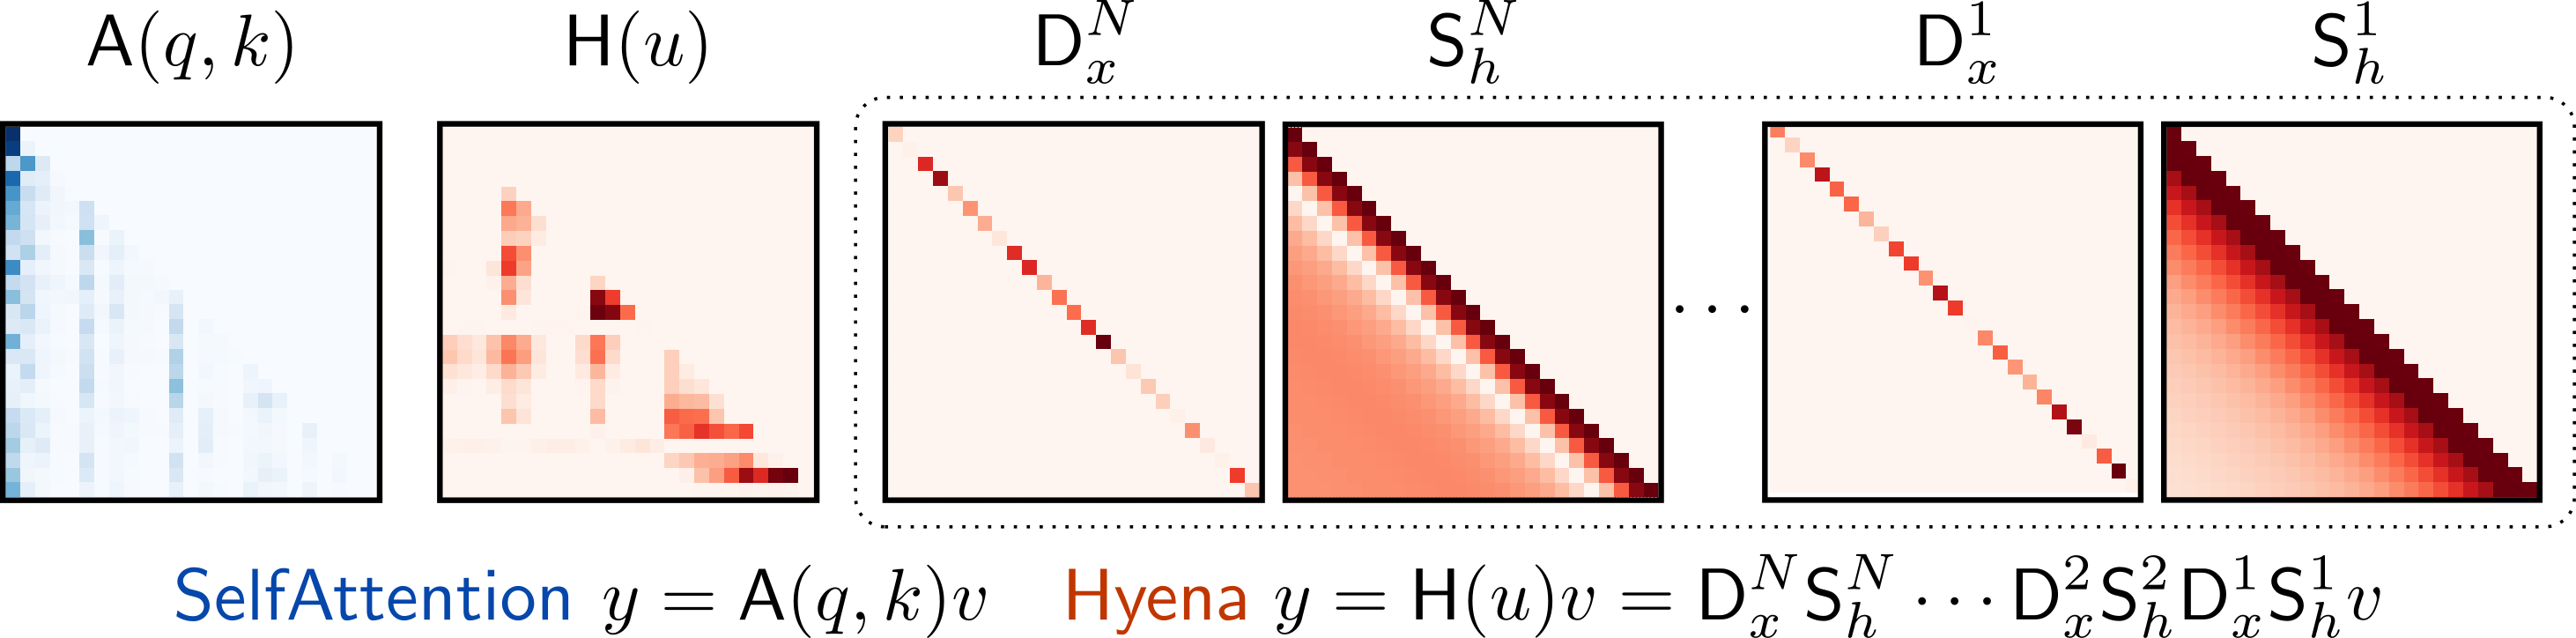
\includegraphics[width=0.69\linewidth]{figures/attention.png}
    \vspace{-2mm}
    \caption{Comparison between data-controlled matrices: $\sf SelfAttention$ and $\sf Hyena$.}
    \label{fig:hyena_matrices}
\end{figure*}
%
where $\sM_q, \sM_k, \sM_v\in\R^{D\x D}$ are learnable linear projections and ${\sf SoftMax}$ is intended to be applied row-wise. Attention parametrizes a \textbf{family of dense linear operators} and for an input $u$, indexes through it via projections of $u$ i.e., $\sA(u)$. We refer to operators of this type as \textit{data-controlled}, as they encode a linear transformation $u \mapsto y$, that is, however, nonlinearly defined by $u$. This approach yields expressive nonlinear operators in $u$, and we hypothesize contributes, together with other mechanisms \citep{olsson2022context}, to the ability of certain operators to learn \textit{in-context} i.e., to adapt to unseen tasks by leveraging context. In deep learning, the projections take on specific names: \textit{query} $q=u\sM_q$, \textit{key} $k=u\sM_k$ and \textit{value} $v = u\sM_v$. We often rewrite the attention operator as $y = \sA(q,k)v$.
%
\begin{remark}
    Similarly to implicit convolutions, $\sf SelfAttention$ does not entangle its ability to access distant information with the number of parameters: it looks at the whole sequence at the price of $\cO(L^2)$ operations.
\end{remark}
%
\paragraph{Subquadratic Operators}
%
Existing approaches to subquadratic alternatives to attention can be summarized by altering the way the data control is implemented i.e., how the operator is nonlinearly defined by $u$, and then applied to $v$. For example, a layer of \textit{Attention-Free Transformers} (AFTs) \citep{zhai2021attention} constructs the operator through a combination of gating and {$\sf SoftMax$} (AFT full) or gating and a single explicit convolution (AFT conv). \textit{Gated State Spaces} (GSS) instead compose the operator via gating and a long convolution parametrized via SSMs. Taking this idea further, \textit{Hungry Hungry Hippo (H3)} \citep{dao2022hungry}, motivated by gaps of GSS on associative recall, extend the mechanism to include an additional gate and a short convolution obtained via a shift SSM. ${\sf Hyena}$ generalizes this body of work by introducing a recurrence of gates and implicit long convolutions, evaluated efficiently.
\section{Hyena: Definition and Properties}\label{allofhyena}
%
In this section, we define Hyena, a class of \textit{data-controlled} operators consisting of a recurrence of multiplicative gating interactions and long convolutions. Instead of seeking an approximation to attention, we guide our design by intentionally incorporating key computational properties of attention, including the decoupling of sequence length and parameter counts.
%
\subsection{${\sf Hyena}$ Recurrences}\label{hyena_op}
%
At a high level, ${\sf Hyena}$ consists of the following steps (setting $D = 1$ for clarity):
\begin{itemize}
    \item[$i.$] Compute a set of $N + 1$ linear projections of the input, similarly to attention. The number of projections $(v_t, x^1_t, \dots, x^N_t)$ need not be three. One projection takes the role of value, such that a linear input-output function can be defined as $y = \sH(u) v$ for some $\sH(u)$.
    \item[$ii.$] The matrix $\sH(u)$ is defined by interleaving implicit long convolutions and element-wise multiplication with one projection $x^i$ at a time, until all projections are exhausted. Evaluation of $\sH(u) v$ is done efficiently \textbf{without materializing} $\sH(u)$. By doing so, we implicitly define a data-controlled operator as a factorization of a matrix. The long convolutions forming $\sH(u)$ are parametrized implicitly to retain sublinear parameter scaling in sequence length.
\end{itemize}
%
Next, we formally define ${\sf Hyena}$, starting with its computational model. We leave the analysis of its data-controlled matrix form for the latter part of the section.
%
\begin{tcolorbox}[enhanced, sharp corners, drop fuzzy shadow, frame hidden, colback=yellow!15]
\begin{definition}[Order--$N$ $\sf Hyena$ Operator] 
Let $(v, x^1, \cdots, x^N)$ be projections of the input and let $h^1,\dots, h^N$ be a set of learnable filters. The ${\sf Hyena}_N$ operator is defined by the recurrence:
%
\begin{equation}\label{eq:hyena}
    \begin{aligned}
        z^1_t &={\ocra v}_t\\
        z^{n+1}_t & = x_t^n (h^n * z^n)_t & n=1,\dots,N\\
        {\color{blue!70}y}_t &= z_t^{N+1}
    \end{aligned} 
\end{equation}
\end{definition}
\end{tcolorbox}
%
\begin{remark}
The time complexity of a $\sf Hyena$ recurrence is $\mathcal{O}(N L \log_2 L)$. The input-output map can be rewritten as 
\[
y = x^N \cdot (h^N * ( x^{N-1} \cdot (h^{N-1} * (\cdots))))
\]
where each convolution is performed through the Fourier domain in $\mathcal{O}(L \log_2 L)$.
\end{remark}
%
Interestingly, the element-wise product in time domain corresponds to convolution in frequency domain, i.e.
%
\[ x_tu_t = (\hat x * \hat u)_t, \]
%
where $\hat x,\hat u$ denote the DFT of $x$ and $u$, respectively. Thus, $\sf Hyena$ is alternatively applying convolutions in the time and then the frequency domain (or alternatively applying element-wise products in the time and frequency domain). One potential explanation for the effectiveness of this procedure is that the convolution in the time domain (element-wise multiplication in the frequency domain) increases the memory length, allowing for a broader context to be taken into account. On the other hand, the element-wise multiplication in the time domain (convolution in the frequency domain) allows for more fine-grained selection of specific frequency components of the signal.
%
\subsection{${\sf Hyena}$ Matrices} 
%
${\sf Hyena}$ operators build on the ${\sf H3}$ mechanism developed by \citep{dao2022hungry}. For clarity of exposition, we once again consider the SISO case ($D=1$). Let $\sD_q$ and $\sD_k$ be the $L$-by-$L$ diagonal matrices whose respective main diagonal entries are the respective entries of $q$ and $k$. ${\sf H3}$ realizes a surrogate attention matrix with a data-controlled, parametrized decomposition in four terms:
%
\begin{equation}\label{eq:linear_attention}
    \begin{aligned}
        \sA(q,k) &= \sD_q \sS_\psi \sD_k \sS_\varphi \\
        {\sf H3}(q, k, v) &= \sA(q,k) v
    \end{aligned}
\end{equation}
%
where $\sS_\varphi,\sS_\psi$ are the Toeplitz matrices of learnable \textbf{causal} filters $\varphi,\psi$ parametrized via SSMs\footnote{For consistency with our discussion, we have swapped $k$ and $v$ compared to the notation in \citep{dao2022hungry}.}. Alongside the $qkv$-projections the filters constitute our degrees of freedom in the layer design. This decomposition allows evaluation of \eqref{eq:linear_attention} in just $\cO(L \log_2 L)$ time (two FFT convolutions and two element-wise products), i.e.
%
\begin{equation}
    \begin{aligned}
        z_{t} &= k_{t}(\varphi * v)_t \\
        y_{t} &= q_{t}(\psi * z)_t
    \end{aligned}
\end{equation}
%
$\small \sf Hyena$ represents a generalization of \eqref{eq:linear_attention} for an arbitrary number of projections -- not limited to three -- and with implicit free-form long filters for the convolutions. The resulting recurrence \eqref{eq:hyena} can be also represented in matrix form $y=\sH(u)v$. Let $\sD_x^n=\diag(x^n)\in\R^{L\x L}$ and let $\sS_h^n$ be the Toeplitz matrix corresponding to filter $h^n$. The resulting $\sf Hyena$ recurrence is linear in $v$ and can be rewritten in matrix form:
%
\[
    y = \sH(u)v = \sD_x^N\sS_h^N \cdots \sD_x^2\sS_h^2\sD_{x}^1\sS_h^1 v
\]
%
Figure~\ref{fig:hyena_matrices} visualizes an example decomposition.
%
\begin{remark}[$\sf Hyena$ generalizes $\sf H3$ and $\sf GSS$.]
    The $\sf H3$ mechanism \citep{dao2022hungry} corresponds to ${\sf Hyena}_2$ and $\sf GSS$ \citep{mehta2022long} is ${\sf Hyena}_{1}$, with a particular choice of parametrization for the long convolutions (SSMs).
\end{remark}
%
Analysis of the $\sf H3$ mechanism as a decomposition $\sD_q\sS_\psi\sD_k\sS_\varphi$ of its surrogate attention matrix\footnote{Some of this analysis is reported in the Appendix.} clarifies a connection to fast evaluation algorithms for matrix-vector multiplications. In particular, the generalization of \eqref{eq:linear_attention} to an arbitrary order is inspired by fast evaluation algorithms for structured dense matrices based on \textit{butterfly} decompositions \citep{li2015butterfly,dao2019learning, dao2022monarch}, with length of the decomposition closely tied to its expressivity (in the classes of matrices it can represent). The ${\sf Hyena}$ operator blends data control with a special case of butterfly decomposition.         
%
\begin{remark}
${\sf Hyena}$ operators have unbounded context. Namely, they are not artificially restricted by e.g., locality, and can learn long-range dependencies between any of the elements of $v$ via long convolutions, which we discuss next.
\end{remark}
%
\subsection{${\sf Hyena}$ Filters}\label{hyena_ker}
%
Here we provide details on the convolution parametrization. We represent the filters of each ${\sf Hyena}$ operator as a map from the time (or space) domain $t$ to values $h_t$, and learn it with a shallow feed-forward neural network ({$\sf FFN$}):
%
\begin{equation}\label{filt}
    h_t = {\sf Window}(t)\cdot({\sf FFN} \circ {\sf PositionalEncoding}) (t)
\end{equation}
%
This approach builds on the neural implicit representation literature \citep{mildenhall2021nerf,sitzmann2020implicit}, which has found application in long convolution layers \citep{romero2021ckconv, romero2021flexconv}. One advantage of \eqref{filt} is given by the decoupling of filter length and parameter cost. 
%
\paragraph{Specializing filters in Hyena}
%
The window and positional encoding functions are used to specialize filters in ${\sf Hyena}$ operators, biasing them towards a specific type. Figure \ref{fig:modul} provides an important example: we choose at least one of the convolutions in ${\sf Hyena}$ to be shaped towards exponential decay, mirroring the findings of \citep{li2022makes} in other applications.
%
\begin{figure}[t]
    \centering
    % This file was created with tikzplotlib v0.10.1.
\begin{tikzpicture}[font=\small]


\definecolor{darkgray176}{RGB}{176,176,176}
\definecolor{dodgerblue}{RGB}{30,144,255}
\definecolor{tomato}{RGB}{255,99,71}

\begin{groupplot}[group style={group size=3 by 1, horizontal sep=0.1cm}]
\nextgroupplot[
width=.4\linewidth, height=3cm,
tick align=outside,
tick pos=left,
title={\(\displaystyle \small{\sf FFN}(t)\)},
title style={yshift=-0.25cm},
x grid style={darkgray176},
xmin=0, xmax=63,
xtick style={color=black},
xtick={-20,0,20,40,60,80},
xticklabels={
  \(\displaystyle {\ensuremath{-}20}\),
  \(\displaystyle {0}\),
  \(\displaystyle {20}\),
  \(\displaystyle {40}\),
  \(\displaystyle {60}\),
  \(\displaystyle {80}\)
},
xlabel={$\small\sf Sequence~Length$},
xlabel style={yshift=0.4cm},
y grid style={darkgray176},
ymin=-1, ymax=1,
ymin=-1, ymax=1,
ytick style={
    /pgfplots/major tick length=0pt,
},
xtick style={
    /pgfplots/major tick length=0pt,
},
ytick={-0.5, 0.5},
xtick={},
xticklabels={},
yticklabels={}
]
\path [draw=tomato, line width=0.5pt]
(axis cs:0,0)
--(axis cs:0,0.0827276557683945);

\path [draw=tomato, line width=0.5pt]
(axis cs:1,0)
--(axis cs:1,-0.286112189292908);

\path [draw=tomato, line width=0.5pt]
(axis cs:2,0)
--(axis cs:2,0.00687235593795776);

\path [draw=tomato, line width=0.5pt]
(axis cs:3,0)
--(axis cs:3,-0.747102022171021);

\path [draw=tomato, line width=0.5pt]
(axis cs:4,0)
--(axis cs:4,0.0641668513417244);

\path [draw=tomato, line width=0.5pt]
(axis cs:5,0)
--(axis cs:5,-0.646571576595306);

\path [draw=tomato, line width=0.5pt]
(axis cs:6,0)
--(axis cs:6,0.0942377746105194);

\path [draw=tomato, line width=0.5pt]
(axis cs:7,0)
--(axis cs:7,0.701024413108826);

\path [draw=tomato, line width=0.5pt]
(axis cs:8,0)
--(axis cs:8,0.218265861272812);

\path [draw=tomato, line width=0.5pt]
(axis cs:9,0)
--(axis cs:9,-0.193984031677246);

\path [draw=tomato, line width=0.5pt]
(axis cs:10,0)
--(axis cs:10,-0.128884062170982);

\path [draw=tomato, line width=0.5pt]
(axis cs:11,0)
--(axis cs:11,0.294504374265671);

\path [draw=tomato, line width=0.5pt]
(axis cs:12,0)
--(axis cs:12,0.597060859203339);

\path [draw=tomato, line width=0.5pt]
(axis cs:13,0)
--(axis cs:13,0.0985148549079895);

\path [draw=tomato, line width=0.5pt]
(axis cs:14,0)
--(axis cs:14,-0.355021268129349);

\path [draw=tomato, line width=0.5pt]
(axis cs:15,0)
--(axis cs:15,0.451927185058594);

\path [draw=tomato, line width=0.5pt]
(axis cs:16,0)
--(axis cs:16,0.051352247595787);

\path [draw=tomato, line width=0.5pt]
(axis cs:17,0)
--(axis cs:17,-0.58028256893158);

\path [draw=tomato, line width=0.5pt]
(axis cs:18,0)
--(axis cs:18,0.37768816947937);

\path [draw=tomato, line width=0.5pt]
(axis cs:19,0)
--(axis cs:19,-0.397529572248459);

\path [draw=tomato, line width=0.5pt]
(axis cs:20,0)
--(axis cs:20,-0.292246282100677);

\path [draw=tomato, line width=0.5pt]
(axis cs:21,0)
--(axis cs:21,0.220617383718491);

\path [draw=tomato, line width=0.5pt]
(axis cs:22,0)
--(axis cs:22,0.196079254150391);

\path [draw=tomato, line width=0.5pt]
(axis cs:23,0)
--(axis cs:23,0.0956322178244591);

\path [draw=tomato, line width=0.5pt]
(axis cs:24,0)
--(axis cs:24,0.45118436217308);

\path [draw=tomato, line width=0.5pt]
(axis cs:25,0)
--(axis cs:25,-0.375823110342026);

\path [draw=tomato, line width=0.5pt]
(axis cs:26,0)
--(axis cs:26,-0.551573514938354);

\path [draw=tomato, line width=0.5pt]
(axis cs:27,0)
--(axis cs:27,0.430078268051147);

\path [draw=tomato, line width=0.5pt]
(axis cs:28,0)
--(axis cs:28,0.279720634222031);

\path [draw=tomato, line width=0.5pt]
(axis cs:29,0)
--(axis cs:29,0.13493886590004);

\path [draw=tomato, line width=0.5pt]
(axis cs:30,0)
--(axis cs:30,-0.149687111377716);

\path [draw=tomato, line width=0.5pt]
(axis cs:31,0)
--(axis cs:31,0.148303136229515);

\path [draw=tomato, line width=0.5pt]
(axis cs:32,0)
--(axis cs:32,-0.219151318073273);

\path [draw=tomato, line width=0.5pt]
(axis cs:33,0)
--(axis cs:33,0.43656313419342);

\path [draw=tomato, line width=0.5pt]
(axis cs:34,0)
--(axis cs:34,-0.168442666530609);

\path [draw=tomato, line width=0.5pt]
(axis cs:35,0)
--(axis cs:35,0.187510102987289);

\path [draw=tomato, line width=0.5pt]
(axis cs:36,0)
--(axis cs:36,0.108915574848652);

\path [draw=tomato, line width=0.5pt]
(axis cs:37,0)
--(axis cs:37,-0.336748242378235);

\path [draw=tomato, line width=0.5pt]
(axis cs:38,0)
--(axis cs:38,0.2141472697258);

\path [draw=tomato, line width=0.5pt]
(axis cs:39,0)
--(axis cs:39,-0.031447671353817);

\path [draw=tomato, line width=0.5pt]
(axis cs:40,0)
--(axis cs:40,-0.348572671413422);

\path [draw=tomato, line width=0.5pt]
(axis cs:41,0)
--(axis cs:41,-0.17571160197258);

\path [draw=tomato, line width=0.5pt]
(axis cs:42,0)
--(axis cs:42,-0.250227987766266);

\path [draw=tomato, line width=0.5pt]
(axis cs:43,0)
--(axis cs:43,-0.0833175778388977);

\path [draw=tomato, line width=0.5pt]
(axis cs:44,0)
--(axis cs:44,0.0600676089525223);

\path [draw=tomato, line width=0.5pt]
(axis cs:45,0)
--(axis cs:45,-0.286332786083221);

\path [draw=tomato, line width=0.5pt]
(axis cs:46,0)
--(axis cs:46,0.0833164602518082);

\path [draw=tomato, line width=0.5pt]
(axis cs:47,0)
--(axis cs:47,0.352049469947815);

\path [draw=tomato, line width=0.5pt]
(axis cs:48,0)
--(axis cs:48,-0.602340042591095);

\path [draw=tomato, line width=0.5pt]
(axis cs:49,0)
--(axis cs:49,0.355826735496521);

\path [draw=tomato, line width=0.5pt]
(axis cs:50,0)
--(axis cs:50,-0.0874901711940765);

\path [draw=tomato, line width=0.5pt]
(axis cs:51,0)
--(axis cs:51,0.290616244077682);

\path [draw=tomato, line width=0.5pt]
(axis cs:52,0)
--(axis cs:52,0.196222603321075);

\path [draw=tomato, line width=0.5pt]
(axis cs:53,0)
--(axis cs:53,0.328381299972534);

\path [draw=tomato, line width=0.5pt]
(axis cs:54,0)
--(axis cs:54,-0.50971782207489);

\path [draw=tomato, line width=0.5pt]
(axis cs:55,0)
--(axis cs:55,0.476836383342743);

\path [draw=tomato, line width=0.5pt]
(axis cs:56,0)
--(axis cs:56,-0.223778992891312);

\path [draw=tomato, line width=0.5pt]
(axis cs:57,0)
--(axis cs:57,0.101644188165665);

\path [draw=tomato, line width=0.5pt]
(axis cs:58,0)
--(axis cs:58,0.260815739631653);

\path [draw=tomato, line width=0.5pt]
(axis cs:59,0)
--(axis cs:59,0.323934018611908);

\path [draw=tomato, line width=0.5pt]
(axis cs:60,0)
--(axis cs:60,-0.025722473859787);

\path [draw=tomato, line width=0.5pt]
(axis cs:61,0)
--(axis cs:61,-0.672560632228851);

\path [draw=tomato, line width=0.5pt]
(axis cs:62,0)
--(axis cs:62,-0.533866047859192);

\path [draw=tomato, line width=0.5pt]
(axis cs:63,0)
--(axis cs:63,0.319244116544724);

\addplot [semithick, tomato, mark=*, , mark size=0.5, mark options={solid}, only marks]
table {%
0 0.0827276557683945
1 -0.286112189292908
2 0.00687235593795776
3 -0.747102022171021
4 0.0641668513417244
5 -0.646571576595306
6 0.0942377746105194
7 0.701024413108826
8 0.218265861272812
9 -0.193984031677246
10 -0.128884062170982
11 0.294504374265671
12 0.597060859203339
13 0.0985148549079895
14 -0.355021268129349
15 0.451927185058594
16 0.051352247595787
17 -0.58028256893158
18 0.37768816947937
19 -0.397529572248459
20 -0.292246282100677
21 0.220617383718491
22 0.196079254150391
23 0.0956322178244591
24 0.45118436217308
25 -0.375823110342026
26 -0.551573514938354
27 0.430078268051147
28 0.279720634222031
29 0.13493886590004
30 -0.149687111377716
31 0.148303136229515
32 -0.219151318073273
33 0.43656313419342
34 -0.168442666530609
35 0.187510102987289
36 0.108915574848652
37 -0.336748242378235
38 0.2141472697258
39 -0.031447671353817
40 -0.348572671413422
41 -0.17571160197258
42 -0.250227987766266
43 -0.0833175778388977
44 0.0600676089525223
45 -0.286332786083221
46 0.0833164602518082
47 0.352049469947815
48 -0.602340042591095
49 0.355826735496521
50 -0.0874901711940765
51 0.290616244077682
52 0.196222603321075
53 0.328381299972534
54 -0.50971782207489
55 0.476836383342743
56 -0.223778992891312
57 0.101644188165665
58 0.260815739631653
59 0.323934018611908
60 -0.025722473859787
61 -0.672560632228851
62 -0.533866047859192
63 0.319244116544724
};
\addplot [semithick, black, opacity=0.5]
table {%
0 0
63 0
};
\path [draw=dodgerblue, line width=0.5pt]
(axis cs:0,0)
--(axis cs:0,-0.157364428043365);

\path [draw=dodgerblue, line width=0.5pt]
(axis cs:1,0)
--(axis cs:1,-0.427482098340988);

\path [draw=dodgerblue, line width=0.5pt]
(axis cs:2,0)
--(axis cs:2,0.142682164907455);

\path [draw=dodgerblue, line width=0.5pt]
(axis cs:3,0)
--(axis cs:3,0.13648484647274);

\path [draw=dodgerblue, line width=0.5pt]
(axis cs:4,0)
--(axis cs:4,-0.280892670154572);

\path [draw=dodgerblue, line width=0.5pt]
(axis cs:5,0)
--(axis cs:5,-0.206416189670563);

\path [draw=dodgerblue, line width=0.5pt]
(axis cs:6,0)
--(axis cs:6,0.547141075134277);

\path [draw=dodgerblue, line width=0.5pt]
(axis cs:7,0)
--(axis cs:7,0.554675102233887);

\path [draw=dodgerblue, line width=0.5pt]
(axis cs:8,0)
--(axis cs:8,0.0811909660696983);

\path [draw=dodgerblue, line width=0.5pt]
(axis cs:9,0)
--(axis cs:9,0.132868245244026);

\path [draw=dodgerblue, line width=0.5pt]
(axis cs:10,0)
--(axis cs:10,0.0273473262786865);

\path [draw=dodgerblue, line width=0.5pt]
(axis cs:11,0)
--(axis cs:11,-0.144984915852547);

\path [draw=dodgerblue, line width=0.5pt]
(axis cs:12,0)
--(axis cs:12,-0.175465166568756);

\path [draw=dodgerblue, line width=0.5pt]
(axis cs:13,0)
--(axis cs:13,-0.596456289291382);

\path [draw=dodgerblue, line width=0.5pt]
(axis cs:14,0)
--(axis cs:14,-0.645349979400635);

\path [draw=dodgerblue, line width=0.5pt]
(axis cs:15,0)
--(axis cs:15,-0.649974942207336);

\path [draw=dodgerblue, line width=0.5pt]
(axis cs:16,0)
--(axis cs:16,0.199487075209618);

\path [draw=dodgerblue, line width=0.5pt]
(axis cs:17,0)
--(axis cs:17,-0.274360179901123);

\path [draw=dodgerblue, line width=0.5pt]
(axis cs:18,0)
--(axis cs:18,0.203906893730164);

\path [draw=dodgerblue, line width=0.5pt]
(axis cs:19,0)
--(axis cs:19,0.152370482683182);

\path [draw=dodgerblue, line width=0.5pt]
(axis cs:20,0)
--(axis cs:20,0.174620300531387);

\path [draw=dodgerblue, line width=0.5pt]
(axis cs:21,0)
--(axis cs:21,0.522812962532043);

\path [draw=dodgerblue, line width=0.5pt]
(axis cs:22,0)
--(axis cs:22,0.0771784633398056);

\path [draw=dodgerblue, line width=0.5pt]
(axis cs:23,0)
--(axis cs:23,0.0874599814414978);

\path [draw=dodgerblue, line width=0.5pt]
(axis cs:24,0)
--(axis cs:24,0.614305555820465);

\path [draw=dodgerblue, line width=0.5pt]
(axis cs:25,0)
--(axis cs:25,0.12136672437191);

\path [draw=dodgerblue, line width=0.5pt]
(axis cs:26,0)
--(axis cs:26,-0.781261801719666);

\path [draw=dodgerblue, line width=0.5pt]
(axis cs:27,0)
--(axis cs:27,-0.270010888576508);

\path [draw=dodgerblue, line width=0.5pt]
(axis cs:28,0)
--(axis cs:28,-0.0632222071290016);

\path [draw=dodgerblue, line width=0.5pt]
(axis cs:29,0)
--(axis cs:29,0.0328346192836761);

\path [draw=dodgerblue, line width=0.5pt]
(axis cs:30,0)
--(axis cs:30,-0.151270389556885);

\path [draw=dodgerblue, line width=0.5pt]
(axis cs:31,0)
--(axis cs:31,0.0907290130853653);

\path [draw=dodgerblue, line width=0.5pt]
(axis cs:32,0)
--(axis cs:32,-0.102379135787487);

\path [draw=dodgerblue, line width=0.5pt]
(axis cs:33,0)
--(axis cs:33,0.172654956579208);

\path [draw=dodgerblue, line width=0.5pt]
(axis cs:34,0)
--(axis cs:34,-0.272154688835144);

\path [draw=dodgerblue, line width=0.5pt]
(axis cs:35,0)
--(axis cs:35,-0.442658245563507);

\path [draw=dodgerblue, line width=0.5pt]
(axis cs:36,0)
--(axis cs:36,-0.277874201536179);

\path [draw=dodgerblue, line width=0.5pt]
(axis cs:37,0)
--(axis cs:37,-0.601137280464172);

\path [draw=dodgerblue, line width=0.5pt]
(axis cs:38,0)
--(axis cs:38,-0.184094831347466);

\path [draw=dodgerblue, line width=0.5pt]
(axis cs:39,0)
--(axis cs:39,-0.611811995506287);

\path [draw=dodgerblue, line width=0.5pt]
(axis cs:40,0)
--(axis cs:40,0.268652617931366);

\path [draw=dodgerblue, line width=0.5pt]
(axis cs:41,0)
--(axis cs:41,0.366888105869293);

\path [draw=dodgerblue, line width=0.5pt]
(axis cs:42,0)
--(axis cs:42,-0.221810460090637);

\path [draw=dodgerblue, line width=0.5pt]
(axis cs:43,0)
--(axis cs:43,-0.288709104061127);

\path [draw=dodgerblue, line width=0.5pt]
(axis cs:44,0)
--(axis cs:44,-0.200994670391083);

\path [draw=dodgerblue, line width=0.5pt]
(axis cs:45,0)
--(axis cs:45,0.205075562000275);

\path [draw=dodgerblue, line width=0.5pt]
(axis cs:46,0)
--(axis cs:46,-0.0766182839870453);

\path [draw=dodgerblue, line width=0.5pt]
(axis cs:47,0)
--(axis cs:47,-0.244192555546761);

\path [draw=dodgerblue, line width=0.5pt]
(axis cs:48,0)
--(axis cs:48,0.0179197043180466);

\path [draw=dodgerblue, line width=0.5pt]
(axis cs:49,0)
--(axis cs:49,0.0930630937218666);

\path [draw=dodgerblue, line width=0.5pt]
(axis cs:50,0)
--(axis cs:50,-0.445823669433594);

\path [draw=dodgerblue, line width=0.5pt]
(axis cs:51,0)
--(axis cs:51,0.254653960466385);

\path [draw=dodgerblue, line width=0.5pt]
(axis cs:52,0)
--(axis cs:52,0.336896419525146);

\path [draw=dodgerblue, line width=0.5pt]
(axis cs:53,0)
--(axis cs:53,0.276561886072159);

\path [draw=dodgerblue, line width=0.5pt]
(axis cs:54,0)
--(axis cs:54,-0.0854888334870338);

\path [draw=dodgerblue, line width=0.5pt]
(axis cs:55,0)
--(axis cs:55,-0.203203588724136);

\path [draw=dodgerblue, line width=0.5pt]
(axis cs:56,0)
--(axis cs:56,-0.0140467137098312);

\path [draw=dodgerblue, line width=0.5pt]
(axis cs:57,0)
--(axis cs:57,0.209479957818985);

\path [draw=dodgerblue, line width=0.5pt]
(axis cs:58,0)
--(axis cs:58,-0.0496293902397156);

\path [draw=dodgerblue, line width=0.5pt]
(axis cs:59,0)
--(axis cs:59,1.01678144931793);

\path [draw=dodgerblue, line width=0.5pt]
(axis cs:60,0)
--(axis cs:60,0.648102879524231);

\path [draw=dodgerblue, line width=0.5pt]
(axis cs:61,0)
--(axis cs:61,-0.590502798557281);

\path [draw=dodgerblue, line width=0.5pt]
(axis cs:62,0)
--(axis cs:62,-0.0975861623883247);

\path [draw=dodgerblue, line width=0.5pt]
(axis cs:63,0)
--(axis cs:63,0.428968280553818);

\addplot [semithick, dodgerblue, mark=*, , mark size=0.5, mark options={solid}, only marks]
table {%
0 -0.157364428043365
1 -0.427482098340988
2 0.142682164907455
3 0.13648484647274
4 -0.280892670154572
5 -0.206416189670563
6 0.547141075134277
7 0.554675102233887
8 0.0811909660696983
9 0.132868245244026
10 0.0273473262786865
11 -0.144984915852547
12 -0.175465166568756
13 -0.596456289291382
14 -0.645349979400635
15 -0.649974942207336
16 0.199487075209618
17 -0.274360179901123
18 0.203906893730164
19 0.152370482683182
20 0.174620300531387
21 0.522812962532043
22 0.0771784633398056
23 0.0874599814414978
24 0.614305555820465
25 0.12136672437191
26 -0.781261801719666
27 -0.270010888576508
28 -0.0632222071290016
29 0.0328346192836761
30 -0.151270389556885
31 0.0907290130853653
32 -0.102379135787487
33 0.172654956579208
34 -0.272154688835144
35 -0.442658245563507
36 -0.277874201536179
37 -0.601137280464172
38 -0.184094831347466
39 -0.611811995506287
40 0.268652617931366
41 0.366888105869293
42 -0.221810460090637
43 -0.288709104061127
44 -0.200994670391083
45 0.205075562000275
46 -0.0766182839870453
47 -0.244192555546761
48 0.0179197043180466
49 0.0930630937218666
50 -0.445823669433594
51 0.254653960466385
52 0.336896419525146
53 0.276561886072159
54 -0.0854888334870338
55 -0.203203588724136
56 -0.0140467137098312
57 0.209479957818985
58 -0.0496293902397156
59 1.01678144931793
60 0.648102879524231
61 -0.590502798557281
62 -0.0975861623883247
63 0.428968280553818
};
\addplot [semithick, black, opacity=0.5]
table {%
0 0
63 0
};

\nextgroupplot[
width=.4\linewidth, height=3cm,
tick align=outside,
tick pos=left,
title={\(\displaystyle \small\sf Window\)},
title style={yshift=-0.21cm},
x grid style={darkgray176},
xmin=0, xmax=63,
xtick style={color=black},
xtick={-25,0,25,50,75},
ymin=-1.2, ymax=1.2,
ytick style={
    /pgfplots/major tick length=0pt,
},
xtick style={
    /pgfplots/major tick length=0pt,
},
xlabel={$\small\sf Sequence~Length$},
xlabel style={yshift=0.4cm},
ytick={},
xtick={},
xticklabels={},
yticklabels={}
]
\path [draw=tomato, line width=0.5pt]
(axis cs:0,0)
--(axis cs:0,1);

\path [draw=tomato, line width=0.5pt]
(axis cs:1,0)
--(axis cs:1,0.92950975894928);

\path [draw=tomato, line width=0.5pt]
(axis cs:2,0)
--(axis cs:2,0.86398845911026);

\path [draw=tomato, line width=0.5pt]
(axis cs:3,0)
--(axis cs:3,0.803085684776306);

\path [draw=tomato, line width=0.5pt]
(axis cs:4,0)
--(axis cs:4,0.746476054191589);

\path [draw=tomato, line width=0.5pt]
(axis cs:5,0)
--(axis cs:5,0.693856775760651);

\path [draw=tomato, line width=0.5pt]
(axis cs:6,0)
--(axis cs:6,0.64494663476944);

\path [draw=tomato, line width=0.5pt]
(axis cs:7,0)
--(axis cs:7,0.599484205245972);

\path [draw=tomato, line width=0.5pt]
(axis cs:8,0)
--(axis cs:8,0.557226479053497);

\path [draw=tomato, line width=0.5pt]
(axis cs:9,0)
--(axis cs:9,0.517947435379028);

\path [draw=tomato, line width=0.5pt]
(axis cs:10,0)
--(axis cs:10,0.481437206268311);

\path [draw=tomato, line width=0.5pt]
(axis cs:11,0)
--(axis cs:11,0.447500586509705);

\path [draw=tomato, line width=0.5pt]
(axis cs:12,0)
--(axis cs:12,0.415956169366837);

\path [draw=tomato, line width=0.5pt]
(axis cs:13,0)
--(axis cs:13,0.386635333299637);

\path [draw=tomato, line width=0.5pt]
(axis cs:14,0)
--(axis cs:14,0.359381347894669);

\path [draw=tomato, line width=0.5pt]
(axis cs:15,0)
--(axis cs:15,0.334048479795456);

\path [draw=tomato, line width=0.5pt]
(axis cs:16,0)
--(axis cs:16,0.310501337051392);

\path [draw=tomato, line width=0.5pt]
(axis cs:17,0)
--(axis cs:17,0.28861403465271);

\path [draw=tomato, line width=0.5pt]
(axis cs:18,0)
--(axis cs:18,0.268269568681717);

\path [draw=tomato, line width=0.5pt]
(axis cs:19,0)
--(axis cs:19,0.249359175562859);

\path [draw=tomato, line width=0.5pt]
(axis cs:20,0)
--(axis cs:20,0.231781795620918);

\path [draw=tomato, line width=0.5pt]
(axis cs:21,0)
--(axis cs:21,0.215443447232246);

\path [draw=tomato, line width=0.5pt]
(axis cs:22,0)
--(axis cs:22,0.200256764888763);

\path [draw=tomato, line width=0.5pt]
(axis cs:23,0)
--(axis cs:23,0.18614062666893);

\path [draw=tomato, line width=0.5pt]
(axis cs:24,0)
--(axis cs:24,0.173019528388977);

\path [draw=tomato, line width=0.5pt]
(axis cs:25,0)
--(axis cs:25,0.160823345184326);

\path [draw=tomato, line width=0.5pt]
(axis cs:26,0)
--(axis cs:26,0.149486869573593);

\path [draw=tomato, line width=0.5pt]
(axis cs:27,0)
--(axis cs:27,0.138949528336525);

\path [draw=tomato, line width=0.5pt]
(axis cs:28,0)
--(axis cs:28,0.129154950380325);

\path [draw=tomato, line width=0.5pt]
(axis cs:29,0)
--(axis cs:29,0.12005078792572);

\path [draw=tomato, line width=0.5pt]
(axis cs:30,0)
--(axis cs:30,0.111588381230831);

\path [draw=tomato, line width=0.5pt]
(axis cs:31,0)
--(axis cs:31,0.103722497820854);

\path [draw=tomato, line width=0.5pt]
(axis cs:32,0)
--(axis cs:32,0.0964110940694809);

\path [draw=tomato, line width=0.5pt]
(axis cs:33,0)
--(axis cs:33,0.0896150544285774);

\path [draw=tomato, line width=0.5pt]
(axis cs:34,0)
--(axis cs:34,0.083298072218895);

\path [draw=tomato, line width=0.5pt]
(axis cs:35,0)
--(axis cs:35,0.0774263739585876);

\path [draw=tomato, line width=0.5pt]
(axis cs:36,0)
--(axis cs:36,0.0719685703516006);

\path [draw=tomato, line width=0.5pt]
(axis cs:37,0)
--(axis cs:37,0.066895492374897);

\path [draw=tomato, line width=0.5pt]
(axis cs:38,0)
--(axis cs:38,0.0621800161898136);

\path [draw=tomato, line width=0.5pt]
(axis cs:39,0)
--(axis cs:39,0.0577969327569008);

\path [draw=tomato, line width=0.5pt]
(axis cs:40,0)
--(axis cs:40,0.0537228137254715);

\path [draw=tomato, line width=0.5pt]
(axis cs:41,0)
--(axis cs:41,0.0499358810484409);

\path [draw=tomato, line width=0.5pt]
(axis cs:42,0)
--(axis cs:42,0.0464158914983273);

\path [draw=tomato, line width=0.5pt]
(axis cs:43,0)
--(axis cs:43,0.0431440249085426);

\path [draw=tomato, line width=0.5pt]
(axis cs:44,0)
--(axis cs:44,0.0401028022170067);

\path [draw=tomato, line width=0.5pt]
(axis cs:45,0)
--(axis cs:45,0.0372759476304054);

\path [draw=tomato, line width=0.5pt]
(axis cs:46,0)
--(axis cs:46,0.0346483588218689);

\path [draw=tomato, line width=0.5pt]
(axis cs:47,0)
--(axis cs:47,0.0322059877216816);

\path [draw=tomato, line width=0.5pt]
(axis cs:48,0)
--(axis cs:48,0.0299357660114765);

\path [draw=tomato, line width=0.5pt]
(axis cs:49,0)
--(axis cs:49,0.0278255939483643);

\path [draw=tomato, line width=0.5pt]
(axis cs:50,0)
--(axis cs:50,0.0258641615509987);

\path [draw=tomato, line width=0.5pt]
(axis cs:51,0)
--(axis cs:51,0.0240409914404154);

\path [draw=tomato, line width=0.5pt]
(axis cs:52,0)
--(axis cs:52,0.0223463363945484);

\path [draw=tomato, line width=0.5pt]
(axis cs:53,0)
--(axis cs:53,0.0207711383700371);

\path [draw=tomato, line width=0.5pt]
(axis cs:54,0)
--(axis cs:54,0.0193069763481617);

\path [draw=tomato, line width=0.5pt]
(axis cs:55,0)
--(axis cs:55,0.0179460234940052);

\path [draw=tomato, line width=0.5pt]
(axis cs:56,0)
--(axis cs:56,0.0166810005903244);

\path [draw=tomato, line width=0.5pt]
(axis cs:57,0)
--(axis cs:57,0.0155051574110985);

\path [draw=tomato, line width=0.5pt]
(axis cs:58,0)
--(axis cs:58,0.014412191696465);

\path [draw=tomato, line width=0.5pt]
(axis cs:59,0)
--(axis cs:59,0.0133962770923972);

\path [draw=tomato, line width=0.5pt]
(axis cs:60,0)
--(axis cs:60,0.0124519672244787);

\path [draw=tomato, line width=0.5pt]
(axis cs:61,0)
--(axis cs:61,0.0115742282941937);

\path [draw=tomato, line width=0.5pt]
(axis cs:62,0)
--(axis cs:62,0.0107583561912179);

\path [draw=tomato, line width=0.5pt]
(axis cs:63,0)
--(axis cs:63,0.00999999977648258);

\addplot [semithick, tomato, mark=*, , mark size=0.5, mark options={solid}, only marks]
table {%
0 1
1 0.92950975894928
2 0.86398845911026
3 0.803085684776306
4 0.746476054191589
5 0.693856775760651
6 0.64494663476944
7 0.599484205245972
8 0.557226479053497
9 0.517947435379028
10 0.481437206268311
11 0.447500586509705
12 0.415956169366837
13 0.386635333299637
14 0.359381347894669
15 0.334048479795456
16 0.310501337051392
17 0.28861403465271
18 0.268269568681717
19 0.249359175562859
20 0.231781795620918
21 0.215443447232246
22 0.200256764888763
23 0.18614062666893
24 0.173019528388977
25 0.160823345184326
26 0.149486869573593
27 0.138949528336525
28 0.129154950380325
29 0.12005078792572
30 0.111588381230831
31 0.103722497820854
32 0.0964110940694809
33 0.0896150544285774
34 0.083298072218895
35 0.0774263739585876
36 0.0719685703516006
37 0.066895492374897
38 0.0621800161898136
39 0.0577969327569008
40 0.0537228137254715
41 0.0499358810484409
42 0.0464158914983273
43 0.0431440249085426
44 0.0401028022170067
45 0.0372759476304054
46 0.0346483588218689
47 0.0322059877216816
48 0.0299357660114765
49 0.0278255939483643
50 0.0258641615509987
51 0.0240409914404154
52 0.0223463363945484
53 0.0207711383700371
54 0.0193069763481617
55 0.0179460234940052
56 0.0166810005903244
57 0.0155051574110985
58 0.014412191696465
59 0.0133962770923972
60 0.0124519672244787
61 0.0115742282941937
62 0.0107583561912179
63 0.00999999977648258
};
\addplot [semithick, black, opacity=0.5]
table {%
0 0
63 0
};
\path [draw=dodgerblue, line width=0.5pt]
(axis cs:0,0)
--(axis cs:0,1);

\path [draw=dodgerblue, line width=0.5pt]
(axis cs:1,0)
--(axis cs:1,0.783754229545593);

\path [draw=dodgerblue, line width=0.5pt]
(axis cs:2,0)
--(axis cs:2,0.614270687103271);

\path [draw=dodgerblue, line width=0.5pt]
(axis cs:3,0)
--(axis cs:3,0.481437206268311);

\path [draw=dodgerblue, line width=0.5pt]
(axis cs:4,0)
--(axis cs:4,0.377328455448151);

\path [draw=dodgerblue, line width=0.5pt]
(axis cs:5,0)
--(axis cs:5,0.295732766389847);

\path [draw=dodgerblue, line width=0.5pt]
(axis cs:6,0)
--(axis cs:6,0.231781795620918);

\path [draw=dodgerblue, line width=0.5pt]
(axis cs:7,0)
--(axis cs:7,0.18165996670723);

\path [draw=dodgerblue, line width=0.5pt]
(axis cs:8,0)
--(axis cs:8,0.142376765608788);

\path [draw=dodgerblue, line width=0.5pt]
(axis cs:9,0)
--(axis cs:9,0.111588381230831);

\path [draw=dodgerblue, line width=0.5pt]
(axis cs:10,0)
--(axis cs:10,0.0874578729271889);

\path [draw=dodgerblue, line width=0.5pt]
(axis cs:11,0)
--(axis cs:11,0.0685454681515694);

\path [draw=dodgerblue, line width=0.5pt]
(axis cs:12,0)
--(axis cs:12,0.0537228025496006);

\path [draw=dodgerblue, line width=0.5pt]
(axis cs:13,0)
--(axis cs:13,0.0421054735779762);

\path [draw=dodgerblue, line width=0.5pt]
(axis cs:14,0)
--(axis cs:14,0.0330003462731838);

\path [draw=dodgerblue, line width=0.5pt]
(axis cs:15,0)
--(axis cs:15,0.0258641559630632);

\path [draw=dodgerblue, line width=0.5pt]
(axis cs:16,0)
--(axis cs:16,0.0202711429446936);

\path [draw=dodgerblue, line width=0.5pt]
(axis cs:17,0)
--(axis cs:17,0.0158875938504934);

\path [draw=dodgerblue, line width=0.5pt]
(axis cs:18,0)
--(axis cs:18,0.0124519672244787);

\path [draw=dodgerblue, line width=0.5pt]
(axis cs:19,0)
--(axis cs:19,0.00975928455591202);

\path [draw=dodgerblue, line width=0.5pt]
(axis cs:20,0)
--(axis cs:20,0.00764887919649482);

\path [draw=dodgerblue, line width=0.5pt]
(axis cs:21,0)
--(axis cs:21,0.00599484331905842);

\path [draw=dodgerblue, line width=0.5pt]
(axis cs:22,0)
--(axis cs:22,0.00469848094508052);

\path [draw=dodgerblue, line width=0.5pt]
(axis cs:23,0)
--(axis cs:23,0.00368245528079569);

\path [draw=dodgerblue, line width=0.5pt]
(axis cs:24,0)
--(axis cs:24,0.00288613932207227);

\path [draw=dodgerblue, line width=0.5pt]
(axis cs:25,0)
--(axis cs:25,0.00226202351041138);

\path [draw=dodgerblue, line width=0.5pt]
(axis cs:26,0)
--(axis cs:26,0.00177287100814283);

\path [draw=dodgerblue, line width=0.5pt]
(axis cs:27,0)
--(axis cs:27,0.00138949486427009);

\path [draw=dodgerblue, line width=0.5pt]
(axis cs:28,0)
--(axis cs:28,0.00108902284409851);

\path [draw=dodgerblue, line width=0.5pt]
(axis cs:29,0)
--(axis cs:29,0.000853526056744158);

\path [draw=dodgerblue, line width=0.5pt]
(axis cs:30,0)
--(axis cs:30,0.000668954569846392);

\path [draw=dodgerblue, line width=0.5pt]
(axis cs:31,0)
--(axis cs:31,0.000524296134244651);

\path [draw=dodgerblue, line width=0.5pt]
(axis cs:32,0)
--(axis cs:32,0.000410919630667195);

\path [draw=dodgerblue, line width=0.5pt]
(axis cs:33,0)
--(axis cs:33,0.000322060077451169);

\path [draw=dodgerblue, line width=0.5pt]
(axis cs:34,0)
--(axis cs:34,0.000252415891736746);

\path [draw=dodgerblue, line width=0.5pt]
(axis cs:35,0)
--(axis cs:35,0.000197831992409192);

\path [draw=dodgerblue, line width=0.5pt]
(axis cs:36,0)
--(axis cs:36,0.000155051631736569);

\path [draw=dodgerblue, line width=0.5pt]
(axis cs:37,0)
--(axis cs:37,0.00012152246927144);

\path [draw=dodgerblue, line width=0.5pt]
(axis cs:38,0)
--(axis cs:38,9.52437330852263e-05);

\path [draw=dodgerblue, line width=0.5pt]
(axis cs:39,0)
--(axis cs:39,7.4647665314842e-05);

\path [draw=dodgerblue, line width=0.5pt]
(axis cs:40,0)
--(axis cs:40,5.85054112889338e-05);

\path [draw=dodgerblue, line width=0.5pt]
(axis cs:41,0)
--(axis cs:41,4.58538561360911e-05);

\path [draw=dodgerblue, line width=0.5pt]
(axis cs:42,0)
--(axis cs:42,3.59381810994819e-05);

\path [draw=dodgerblue, line width=0.5pt]
(axis cs:43,0)
--(axis cs:43,2.81666962109739e-05);

\path [draw=dodgerblue, line width=0.5pt]
(axis cs:44,0)
--(axis cs:44,2.20757628994761e-05);

\path [draw=dodgerblue, line width=0.5pt]
(axis cs:45,0)
--(axis cs:45,1.73019689100329e-05);

\path [draw=dodgerblue, line width=0.5pt]
(axis cs:46,0)
--(axis cs:46,1.35604896058794e-05);

\path [draw=dodgerblue, line width=0.5pt]
(axis cs:47,0)
--(axis cs:47,1.06280995169072e-05);

\path [draw=dodgerblue, line width=0.5pt]
(axis cs:48,0)
--(axis cs:48,8.32980822451646e-06);

\path [draw=dodgerblue, line width=0.5pt]
(axis cs:49,0)
--(axis cs:49,6.52852122584591e-06);

\path [draw=dodgerblue, line width=0.5pt]
(axis cs:50,0)
--(axis cs:50,5.11675534653477e-06);

\path [draw=dodgerblue, line width=0.5pt]
(axis cs:51,0)
--(axis cs:51,4.01028182750451e-06);

\path [draw=dodgerblue, line width=0.5pt]
(axis cs:52,0)
--(axis cs:52,3.14307453663787e-06);

\path [draw=dodgerblue, line width=0.5pt]
(axis cs:53,0)
--(axis cs:53,2.46339754994551e-06);

\path [draw=dodgerblue, line width=0.5pt]
(axis cs:54,0)
--(axis cs:54,1.93069786291744e-06);

\path [draw=dodgerblue, line width=0.5pt]
(axis cs:55,0)
--(axis cs:55,1.51319238739234e-06);

\path [draw=dodgerblue, line width=0.5pt]
(axis cs:56,0)
--(axis cs:56,1.18597188247804e-06);

\path [draw=dodgerblue, line width=0.5pt]
(axis cs:57,0)
--(axis cs:57,9.29510292735358e-07);

\path [draw=dodgerblue, line width=0.5pt]
(axis cs:58,0)
--(axis cs:58,7.28507473013451e-07);

\path [draw=dodgerblue, line width=0.5pt]
(axis cs:59,0)
--(axis cs:59,5.70970712487906e-07);

\path [draw=dodgerblue, line width=0.5pt]
(axis cs:60,0)
--(axis cs:60,4.47500639211285e-07);

\path [draw=dodgerblue, line width=0.5pt]
(axis cs:61,0)
--(axis cs:61,3.50730772424868e-07);

\path [draw=dodgerblue, line width=0.5pt]
(axis cs:62,0)
--(axis cs:62,2.7488667342368e-07);

\path [draw=dodgerblue, line width=0.5pt]
(axis cs:63,0)
--(axis cs:63,2.15443563433837e-07);

\addplot [semithick, dodgerblue, mark=*, , mark size=0.5, mark options={solid}, only marks]
table {%
0 1
1 0.783754229545593
2 0.614270687103271
3 0.481437206268311
4 0.377328455448151
5 0.295732766389847
6 0.231781795620918
7 0.18165996670723
8 0.142376765608788
9 0.111588381230831
10 0.0874578729271889
11 0.0685454681515694
12 0.0537228025496006
13 0.0421054735779762
14 0.0330003462731838
15 0.0258641559630632
16 0.0202711429446936
17 0.0158875938504934
18 0.0124519672244787
19 0.00975928455591202
20 0.00764887919649482
21 0.00599484331905842
22 0.00469848094508052
23 0.00368245528079569
24 0.00288613932207227
25 0.00226202351041138
26 0.00177287100814283
27 0.00138949486427009
28 0.00108902284409851
29 0.000853526056744158
30 0.000668954569846392
31 0.000524296134244651
32 0.000410919630667195
33 0.000322060077451169
34 0.000252415891736746
35 0.000197831992409192
36 0.000155051631736569
37 0.00012152246927144
38 9.52437330852263e-05
39 7.4647665314842e-05
40 5.85054112889338e-05
41 4.58538561360911e-05
42 3.59381810994819e-05
43 2.81666962109739e-05
44 2.20757628994761e-05
45 1.73019689100329e-05
46 1.35604896058794e-05
47 1.06280995169072e-05
48 8.32980822451646e-06
49 6.52852122584591e-06
50 5.11675534653477e-06
51 4.01028182750451e-06
52 3.14307453663787e-06
53 2.46339754994551e-06
54 1.93069786291744e-06
55 1.51319238739234e-06
56 1.18597188247804e-06
57 9.29510292735358e-07
58 7.28507473013451e-07
59 5.70970712487906e-07
60 4.47500639211285e-07
61 3.50730772424868e-07
62 2.7488667342368e-07
63 2.15443563433837e-07
};
\addplot [semithick, black, opacity=0.5]
table {%
0 0
63 0
};

\nextgroupplot[
width=.4\linewidth, height=3cm,
tick align=outside,
tick pos=left,
title={\(\displaystyle {\small\sf Window} \circ {\small\sf FFN}(t)\)},
title style={yshift=-0.3cm},
x grid style={darkgray176},
xmin=0, xmax=63,
xtick style={color=black},
xtick={-25,0,25,50,75},
xticklabels={
  \(\displaystyle {\ensuremath{-}25}\),
  \(\displaystyle {0}\),
  \(\displaystyle {25}\),
  \(\displaystyle {50}\),
  \(\displaystyle {75}\)
},
xlabel={$\small\sf Sequence~Length$},
xlabel style={yshift=0.4cm},
y grid style={darkgray176},
ymin=-0.5, ymax=0.5,
ytick style={
    /pgfplots/major tick length=0pt,
},
xtick style={
    /pgfplots/major tick length=0pt,
},
ytick={},
xtick={},
xticklabels={},
yticklabels={}
]
\path [draw=tomato, line width=0.5pt]
(axis cs:0,0)
--(axis cs:0,0.0827276557683945);

\path [draw=tomato, line width=0.5pt]
(axis cs:1,0)
--(axis cs:1,-0.265944063663483);

\path [draw=tomato, line width=0.5pt]
(axis cs:2,0)
--(axis cs:2,0.00593763636425138);

\path [draw=tomato, line width=0.5pt]
(axis cs:3,0)
--(axis cs:3,-0.599986910820007);

\path [draw=tomato, line width=0.5pt]
(axis cs:4,0)
--(axis cs:4,0.0478990189731121);

\path [draw=tomato, line width=0.5pt]
(axis cs:5,0)
--(axis cs:5,-0.448628067970276);

\path [draw=tomato, line width=0.5pt]
(axis cs:6,0)
--(axis cs:6,0.060778334736824);

\path [draw=tomato, line width=0.5pt]
(axis cs:7,0)
--(axis cs:7,0.420253068208694);

\path [draw=tomato, line width=0.5pt]
(axis cs:8,0)
--(axis cs:8,0.121623516082764);

\path [draw=tomato, line width=0.5pt]
(axis cs:9,0)
--(axis cs:9,-0.100473530590534);

\path [draw=tomato, line width=0.5pt]
(axis cs:10,0)
--(axis cs:10,-0.0620495826005936);

\path [draw=tomato, line width=0.5pt]
(axis cs:11,0)
--(axis cs:11,0.13179087638855);

\path [draw=tomato, line width=0.5pt]
(axis cs:12,0)
--(axis cs:12,0.248351141810417);

\path [draw=tomato, line width=0.5pt]
(axis cs:13,0)
--(axis cs:13,0.0380893237888813);

\path [draw=tomato, line width=0.5pt]
(axis cs:14,0)
--(axis cs:14,-0.127588018774986);

\path [draw=tomato, line width=0.5pt]
(axis cs:15,0)
--(axis cs:15,0.150965586304665);

\path [draw=tomato, line width=0.5pt]
(axis cs:16,0)
--(axis cs:16,0.015944940969348);

\path [draw=tomato, line width=0.5pt]
(axis cs:17,0)
--(axis cs:17,-0.167477697134018);

\path [draw=tomato, line width=0.5pt]
(axis cs:18,0)
--(axis cs:18,0.101322241127491);

\path [draw=tomato, line width=0.5pt]
(axis cs:19,0)
--(axis cs:19,-0.0991276428103447);

\path [draw=tomato, line width=0.5pt]
(axis cs:20,0)
--(axis cs:20,-0.0677373707294464);

\path [draw=tomato, line width=0.5pt]
(axis cs:21,0)
--(axis cs:21,0.0475305691361427);

\path [draw=tomato, line width=0.5pt]
(axis cs:22,0)
--(axis cs:22,0.0392661988735199);

\path [draw=tomato, line width=0.5pt]
(axis cs:23,0)
--(axis cs:23,0.0178010407835245);

\path [draw=tomato, line width=0.5pt]
(axis cs:24,0)
--(axis cs:24,0.0780637040734291);

\path [draw=tomato, line width=0.5pt]
(axis cs:25,0)
--(axis cs:25,-0.0604411289095879);

\path [draw=tomato, line width=0.5pt]
(axis cs:26,0)
--(axis cs:26,-0.0824529975652695);

\path [draw=tomato, line width=0.5pt]
(axis cs:27,0)
--(axis cs:27,0.0597591735422611);

\path [draw=tomato, line width=0.5pt]
(axis cs:28,0)
--(axis cs:28,0.0361273027956486);

\path [draw=tomato, line width=0.5pt]
(axis cs:29,0)
--(axis cs:29,0.0161995179951191);

\path [draw=tomato, line width=0.5pt]
(axis cs:30,0)
--(axis cs:30,-0.0167033430188894);

\path [draw=tomato, line width=0.5pt]
(axis cs:31,0)
--(axis cs:31,0.0153823718428612);

\path [draw=tomato, line width=0.5pt]
(axis cs:32,0)
--(axis cs:32,-0.0211286190897226);

\path [draw=tomato, line width=0.5pt]
(axis cs:33,0)
--(axis cs:33,0.0391226299107075);

\path [draw=tomato, line width=0.5pt]
(axis cs:34,0)
--(axis cs:34,-0.0140309492126107);

\path [draw=tomato, line width=0.5pt]
(axis cs:35,0)
--(axis cs:35,0.0145182274281979);

\path [draw=tomato, line width=0.5pt]
(axis cs:36,0)
--(axis cs:36,0.00783849786967039);

\path [draw=tomato, line width=0.5pt]
(axis cs:37,0)
--(axis cs:37,-0.022526940330863);

\path [draw=tomato, line width=0.5pt]
(axis cs:38,0)
--(axis cs:38,0.01331568043679);

\path [draw=tomato, line width=0.5pt]
(axis cs:39,0)
--(axis cs:39,-0.0018175789155066);

\path [draw=tomato, line width=0.5pt]
(axis cs:40,0)
--(axis cs:40,-0.0187263041734695);

\path [draw=tomato, line width=0.5pt]
(axis cs:41,0)
--(axis cs:41,-0.00877431407570839);

\path [draw=tomato, line width=0.5pt]
(axis cs:42,0)
--(axis cs:42,-0.0116145554929972);

\path [draw=tomato, line width=0.5pt]
(axis cs:43,0)
--(axis cs:43,-0.00359465554356575);

\path [draw=tomato, line width=0.5pt]
(axis cs:44,0)
--(axis cs:44,0.00240887934342027);

\path [draw=tomato, line width=0.5pt]
(axis cs:45,0)
--(axis cs:45,-0.0106733255088329);

\path [draw=tomato, line width=0.5pt]
(axis cs:46,0)
--(axis cs:46,0.00288677867501974);

\path [draw=tomato, line width=0.5pt]
(axis cs:47,0)
--(axis cs:47,0.0113381007686257);

\path [draw=tomato, line width=0.5pt]
(axis cs:48,0)
--(axis cs:48,-0.0180315114557743);

\path [draw=tomato, line width=0.5pt]
(axis cs:49,0)
--(axis cs:49,0.00990109052509069);

\path [draw=tomato, line width=0.5pt]
(axis cs:50,0)
--(axis cs:50,-0.00226285983808339);

\path [draw=tomato, line width=0.5pt]
(axis cs:51,0)
--(axis cs:51,0.00698670279234648);

\path [draw=tomato, line width=0.5pt]
(axis cs:52,0)
--(axis cs:52,0.00438485620543361);

\path [draw=tomato, line width=0.5pt]
(axis cs:53,0)
--(axis cs:53,0.00682085333392024);

\path [draw=tomato, line width=0.5pt]
(axis cs:54,0)
--(axis cs:54,-0.00984110962599516);

\path [draw=tomato, line width=0.5pt]
(axis cs:55,0)
--(axis cs:55,0.00855731684714556);

\path [draw=tomato, line width=0.5pt]
(axis cs:56,0)
--(axis cs:56,-0.00373285752721131);

\path [draw=tomato, line width=0.5pt]
(axis cs:57,0)
--(axis cs:57,0.00157600909005851);

\path [draw=tomato, line width=0.5pt]
(axis cs:58,0)
--(axis cs:58,0.00375892641022801);

\path [draw=tomato, line width=0.5pt]
(axis cs:59,0)
--(axis cs:59,0.00433950964361429);

\path [draw=tomato, line width=0.5pt]
(axis cs:60,0)
--(axis cs:60,-0.000320295395795256);

\path [draw=tomato, line width=0.5pt]
(axis cs:61,0)
--(axis cs:61,-0.00778437033295631);

\path [draw=tomato, line width=0.5pt]
(axis cs:62,0)
--(axis cs:62,-0.00574352126568556);

\path [draw=tomato, line width=0.5pt]
(axis cs:63,0)
--(axis cs:63,0.00319244107231498);

\addplot [semithick, tomato, mark=*, , mark size=0.5, mark options={solid}, only marks]
table {%
0 0.0827276557683945
1 -0.265944063663483
2 0.00593763636425138
3 -0.599986910820007
4 0.0478990189731121
5 -0.448628067970276
6 0.060778334736824
7 0.420253068208694
8 0.121623516082764
9 -0.100473530590534
10 -0.0620495826005936
11 0.13179087638855
12 0.248351141810417
13 0.0380893237888813
14 -0.127588018774986
15 0.150965586304665
16 0.015944940969348
17 -0.167477697134018
18 0.101322241127491
19 -0.0991276428103447
20 -0.0677373707294464
21 0.0475305691361427
22 0.0392661988735199
23 0.0178010407835245
24 0.0780637040734291
25 -0.0604411289095879
26 -0.0824529975652695
27 0.0597591735422611
28 0.0361273027956486
29 0.0161995179951191
30 -0.0167033430188894
31 0.0153823718428612
32 -0.0211286190897226
33 0.0391226299107075
34 -0.0140309492126107
35 0.0145182274281979
36 0.00783849786967039
37 -0.022526940330863
38 0.01331568043679
39 -0.0018175789155066
40 -0.0187263041734695
41 -0.00877431407570839
42 -0.0116145554929972
43 -0.00359465554356575
44 0.00240887934342027
45 -0.0106733255088329
46 0.00288677867501974
47 0.0113381007686257
48 -0.0180315114557743
49 0.00990109052509069
50 -0.00226285983808339
51 0.00698670279234648
52 0.00438485620543361
53 0.00682085333392024
54 -0.00984110962599516
55 0.00855731684714556
56 -0.00373285752721131
57 0.00157600909005851
58 0.00375892641022801
59 0.00433950964361429
60 -0.000320295395795256
61 -0.00778437033295631
62 -0.00574352126568556
63 0.00319244107231498
};
\addplot [semithick, black, opacity=0.5]
table {%
0 0
63 0
};
\path [draw=dodgerblue, line width=0.5pt]
(axis cs:0,0)
--(axis cs:0,-0.157364428043365);

\path [draw=dodgerblue, line width=0.5pt]
(axis cs:1,0)
--(axis cs:1,-0.335040897130966);

\path [draw=dodgerblue, line width=0.5pt]
(axis cs:2,0)
--(axis cs:2,0.0876454710960388);

\path [draw=dodgerblue, line width=0.5pt]
(axis cs:3,0)
--(axis cs:3,0.0657088831067085);

\path [draw=dodgerblue, line width=0.5pt]
(axis cs:4,0)
--(axis cs:4,-0.105988800525665);

\path [draw=dodgerblue, line width=0.5pt]
(axis cs:5,0)
--(axis cs:5,-0.0610440298914909);

\path [draw=dodgerblue, line width=0.5pt]
(axis cs:6,0)
--(axis cs:6,0.126817345619202);

\path [draw=dodgerblue, line width=0.5pt]
(axis cs:7,0)
--(axis cs:7,0.100762262940407);

\path [draw=dodgerblue, line width=0.5pt]
(axis cs:8,0)
--(axis cs:8,0.0115597071126103);

\path [draw=dodgerblue, line width=0.5pt]
(axis cs:9,0)
--(axis cs:9,0.0148265520110726);

\path [draw=dodgerblue, line width=0.5pt]
(axis cs:10,0)
--(axis cs:10,0.0023917390499264);

\path [draw=dodgerblue, line width=0.5pt]
(axis cs:11,0)
--(axis cs:11,-0.00993805937469006);

\path [draw=dodgerblue, line width=0.5pt]
(axis cs:12,0)
--(axis cs:12,-0.00942648015916348);

\path [draw=dodgerblue, line width=0.5pt]
(axis cs:13,0)
--(axis cs:13,-0.0251140743494034);

\path [draw=dodgerblue, line width=0.5pt]
(axis cs:14,0)
--(axis cs:14,-0.0212967731058598);

\path [draw=dodgerblue, line width=0.5pt]
(axis cs:15,0)
--(axis cs:15,-0.016811054199934);

\path [draw=dodgerblue, line width=0.5pt]
(axis cs:16,0)
--(axis cs:16,0.00404383102431893);

\path [draw=dodgerblue, line width=0.5pt]
(axis cs:17,0)
--(axis cs:17,-0.00435892306268215);

\path [draw=dodgerblue, line width=0.5pt]
(axis cs:18,0)
--(axis cs:18,0.0025390419177711);

\path [draw=dodgerblue, line width=0.5pt]
(axis cs:19,0)
--(axis cs:19,0.00148702692240477);

\path [draw=dodgerblue, line width=0.5pt]
(axis cs:20,0)
--(axis cs:20,0.00133564963471144);

\path [draw=dodgerblue, line width=0.5pt]
(axis cs:21,0)
--(axis cs:21,0.00313418172299862);

\path [draw=dodgerblue, line width=0.5pt]
(axis cs:22,0)
--(axis cs:22,0.000362621532985941);

\path [draw=dodgerblue, line width=0.5pt]
(axis cs:23,0)
--(axis cs:23,0.000322067469824106);

\path [draw=dodgerblue, line width=0.5pt]
(axis cs:24,0)
--(axis cs:24,0.00177297147456557);

\path [draw=dodgerblue, line width=0.5pt]
(axis cs:25,0)
--(axis cs:25,0.000274534395430237);

\path [draw=dodgerblue, line width=0.5pt]
(axis cs:26,0)
--(axis cs:26,-0.00138507643714547);

\path [draw=dodgerblue, line width=0.5pt]
(axis cs:27,0)
--(axis cs:27,-0.000375178729882464);

\path [draw=dodgerblue, line width=0.5pt]
(axis cs:28,0)
--(axis cs:28,-6.88504296704195e-05);

\path [draw=dodgerblue, line width=0.5pt]
(axis cs:29,0)
--(axis cs:29,2.80252024822403e-05);

\path [draw=dodgerblue, line width=0.5pt]
(axis cs:30,0)
--(axis cs:30,-0.00010119302169187);

\path [draw=dodgerblue, line width=0.5pt]
(axis cs:31,0)
--(axis cs:31,4.75688721053302e-05);

\path [draw=dodgerblue, line width=0.5pt]
(axis cs:32,0)
--(axis cs:32,-4.2069597839145e-05);

\path [draw=dodgerblue, line width=0.5pt]
(axis cs:33,0)
--(axis cs:33,5.56052691536024e-05);

\path [draw=dodgerblue, line width=0.5pt]
(axis cs:34,0)
--(axis cs:34,-6.86961720930412e-05);

\path [draw=dodgerblue, line width=0.5pt]
(axis cs:35,0)
--(axis cs:35,-8.75719633768313e-05);

\path [draw=dodgerblue, line width=0.5pt]
(axis cs:36,0)
--(axis cs:36,-4.30848485848401e-05);

\path [draw=dodgerblue, line width=0.5pt]
(axis cs:37,0)
--(axis cs:37,-7.30516840121709e-05);

\path [draw=dodgerblue, line width=0.5pt]
(axis cs:38,0)
--(axis cs:38,-1.75338791450486e-05);

\path [draw=dodgerblue, line width=0.5pt]
(axis cs:39,0)
--(axis cs:39,-4.56703382951673e-05);

\path [draw=dodgerblue, line width=0.5pt]
(axis cs:40,0)
--(axis cs:40,1.57176327775232e-05);

\path [draw=dodgerblue, line width=0.5pt]
(axis cs:41,0)
--(axis cs:41,1.68232345458819e-05);

\path [draw=dodgerblue, line width=0.5pt]
(axis cs:42,0)
--(axis cs:42,-7.97146458353382e-06);

\path [draw=dodgerblue, line width=0.5pt]
(axis cs:43,0)
--(axis cs:43,-8.13198130344972e-06);

\path [draw=dodgerblue, line width=0.5pt]
(axis cs:44,0)
--(axis cs:44,-4.43711087427801e-06);

\path [draw=dodgerblue, line width=0.5pt]
(axis cs:45,0)
--(axis cs:45,3.5482109979057e-06);

\path [draw=dodgerblue, line width=0.5pt]
(axis cs:46,0)
--(axis cs:46,-1.03898139514058e-06);

\path [draw=dodgerblue, line width=0.5pt]
(axis cs:47,0)
--(axis cs:47,-2.59530270341202e-06);

\path [draw=dodgerblue, line width=0.5pt]
(axis cs:48,0)
--(axis cs:48,1.49267705751299e-07);

\path [draw=dodgerblue, line width=0.5pt]
(axis cs:49,0)
--(axis cs:49,6.07564402343996e-07);

\path [draw=dodgerblue, line width=0.5pt]
(axis cs:50,0)
--(axis cs:50,-2.28117073675094e-06);

\path [draw=dodgerblue, line width=0.5pt]
(axis cs:51,0)
--(axis cs:51,1.02123419765121e-06);

\path [draw=dodgerblue, line width=0.5pt]
(axis cs:52,0)
--(axis cs:52,1.0588905752229e-06);

\path [draw=dodgerblue, line width=0.5pt]
(axis cs:53,0)
--(axis cs:53,6.81281846937054e-07);

\path [draw=dodgerblue, line width=0.5pt]
(axis cs:54,0)
--(axis cs:54,-1.65053108958091e-07);

\path [draw=dodgerblue, line width=0.5pt]
(axis cs:55,0)
--(axis cs:55,-3.07486118344968e-07);

\path [draw=dodgerblue, line width=0.5pt]
(axis cs:56,0)
--(axis cs:56,-1.66590066186245e-08);

\path [draw=dodgerblue, line width=0.5pt]
(axis cs:57,0)
--(axis cs:57,1.94713777545985e-07);

\path [draw=dodgerblue, line width=0.5pt]
(axis cs:58,0)
--(axis cs:58,-3.61553809113957e-08);

\path [draw=dodgerblue, line width=0.5pt]
(axis cs:59,0)
--(axis cs:59,5.8055240970134e-07);

\path [draw=dodgerblue, line width=0.5pt]
(axis cs:60,0)
--(axis cs:60,2.90026463289905e-07);

\path [draw=dodgerblue, line width=0.5pt]
(axis cs:61,0)
--(axis cs:61,-2.07107504479609e-07);

\path [draw=dodgerblue, line width=0.5pt]
(axis cs:62,0)
--(axis cs:62,-2.68251358903626e-08);

\path [draw=dodgerblue, line width=0.5pt]
(axis cs:63,0)
--(axis cs:63,9.24184533346306e-08);

\addplot [semithick, dodgerblue, mark=*, , mark size=0.5, mark options={solid}, only marks]
table {%
0 -0.157364428043365
1 -0.335040897130966
2 0.0876454710960388
3 0.0657088831067085
4 -0.105988800525665
5 -0.0610440298914909
6 0.126817345619202
7 0.100762262940407
8 0.0115597071126103
9 0.0148265520110726
10 0.0023917390499264
11 -0.00993805937469006
12 -0.00942648015916348
13 -0.0251140743494034
14 -0.0212967731058598
15 -0.016811054199934
16 0.00404383102431893
17 -0.00435892306268215
18 0.0025390419177711
19 0.00148702692240477
20 0.00133564963471144
21 0.00313418172299862
22 0.000362621532985941
23 0.000322067469824106
24 0.00177297147456557
25 0.000274534395430237
26 -0.00138507643714547
27 -0.000375178729882464
28 -6.88504296704195e-05
29 2.80252024822403e-05
30 -0.00010119302169187
31 4.75688721053302e-05
32 -4.2069597839145e-05
33 5.56052691536024e-05
34 -6.86961720930412e-05
35 -8.75719633768313e-05
36 -4.30848485848401e-05
37 -7.30516840121709e-05
38 -1.75338791450486e-05
39 -4.56703382951673e-05
40 1.57176327775232e-05
41 1.68232345458819e-05
42 -7.97146458353382e-06
43 -8.13198130344972e-06
44 -4.43711087427801e-06
45 3.5482109979057e-06
46 -1.03898139514058e-06
47 -2.59530270341202e-06
48 1.49267705751299e-07
49 6.07564402343996e-07
50 -2.28117073675094e-06
51 1.02123419765121e-06
52 1.0588905752229e-06
53 6.81281846937054e-07
54 -1.65053108958091e-07
55 -3.07486118344968e-07
56 -1.66590066186245e-08
57 1.94713777545985e-07
58 -3.61553809113957e-08
59 5.8055240970134e-07
60 2.90026463289905e-07
61 -2.07107504479609e-07
62 -2.68251358903626e-08
63 9.24184533346306e-08
};
\addplot [semithick, black, opacity=0.5]
table {%
0 0
63 0
};
\end{groupplot}

\end{tikzpicture}

    \vspace{-4mm}
    \caption{\textbf{[Top]:} Example of long convolution parametrization for ${\sf Hyena}$ operators, with a decay ${\sf Window}(t) = \exp\{- \alpha t\}$. Parameter $\alpha$ is modified across the independent channels of ${\sf Hyena}$ to regularize filters to be of different lengths. In practice, we add a bias term to our window, so that the filters are not constrained to be zeros after a length determined by the decay rate. 
    }
    \vspace{-4mm}
    \label{fig:modul}
\end{figure}
%
Interestingly, we find that long exponentially decaying filters display synergy with high-frequency filters, as they enable the operator to select specific inputs at specific steps\footnote{This observation finds mirrors in the parametrization of the convolutions in H3 \citep{dao2022hungry} as a shift SSM and a diagonal SSM.}. Similarly to \citep{romero2021ckconv}, we use high-frequency periodic activations (sine) in the {$\sf FFN$}. This allows \eqref{filt} to learn filters with high-frequency content, addressing the low-frequency bias of neural networks \citep{basri2020frequency}.
%
Owing to the {$\sf FFN$}, the parametrization in \eqref{filt} can approximate filters obtained through other means, such as S4 \citep{gu2020hippo,gu2021efficiently}, CKConv \citep{romero2021ckconv}, SGConv \citep{li2022makes} and \textit{Fourier Neural Operator} (FNO) \citep{li2020fourier}.
%

\paragraph{Preserving causality}
%
Causality is necessary to train autoregressive language models, in order for the output at a given position to depend only on the past. For example, Transformers mask the attention matrix to be lower triangular. In the case of ${\sf Hyena}$, causality can be guaranteed by parametrizing causal convolutions: 
%
\begin{proposition}[Causal Hyenas]\label{prop:causality}
    If each filter $h^n, ~n=1,\dots, N$ is causal, then the corresponding ${\sf Hyena}_N$ operator is causal.
    %
\end{proposition}
%
In practice, we need not constrain the learning of the filter \eqref{filt} to ensure its \textit{numerical} causality. If we use FFT-based convolution algorithms, all we need is to evaluate the filter at $t=0,\dots,L-1$ and zero-pad the input and filter sequences to $2 L - 1$ before taking FFT. 
%
\paragraph{Efficiency}
%
One bottleneck of long convolution models can be their low utilization of hardware accelerators, especially when they involve iterative numerical methods to materialize the filter\footnote{In contrast, deep learning primitives are designed for high GPU utilization, with {\sf FFNs} and attention usually reaching $50-70\%$ or higher, if optimized.}. Evaluation of \ref{filt} is fast, since it involves a single forward pass of an {$\sf FFN$}, and can be performed in parallel across sequence length and all orders of an ${\sf Hyena}$ operator as displayed in Algorithm \ref{alg:hyenaa}, increasing hardware utilization. An additional source of low utilization is the FFT, which is also shared by other long other convolutional layers. This bottleneck can be partially addressed by blocking \citep{selesnick2017fast}, and optimization of the underlying routines \citep{dao2022hungry}. We benchmark runtime in Section \ref{benchm}.
%

\subsection{{\sf Hyena} Algorithm}
%

A forward pass of {\sf Hyena} is summarized below. 

\setcounter{algorithm}{-1}
\begin{algorithm}[h]
    \caption{{\sf Projection}}\label{alg:hyenaa}
    \caption{{\sf Projection}}
    \begin{algorithmic}
    \REQUIRE Input sequence $u \in \R^{L \times D}$ \\ 
    \STATE {\small 1.} In parallel across $L$: $\hat{z} = {\sf Linear}(u)$, ${\sf Linear}:\R^{D} \rightarrow \R^{(N+1)D}$ \\
    \STATE {\small 2.} In parallel across $D$: $z = {\sf DepthwiseConv1d}(h, \hat{z} )$, $h$ is a short convolution filter \\
    \STATE {\small 3.} Reshape and split $z$ into $x^1, \dots, x^N, v$. Dimensions of one element are $x^n \in \R^{D \times L}$\\ 
    \STATE Return $x^1, \dots, x^N, v$, $x^n$
    \end{algorithmic}
\end{algorithm}

\setcounter{algorithm}{0}
\begin{algorithm}[h]
    \caption{${\sf HyenaFilter}$}\label{alg:hyenaa}
    \caption{${\sf Hyena}$ Filter}
    \begin{algorithmic}
    \REQUIRE Sequence length $L$, positional embedding dimension $D_e$ \\ 
    \STATE {\small 1.} $t  = {\sf PositionalEncoding}(L)$, $t \in \R^{L \times D_e}$ \\
    \STATE {\small 2.} In parallel across $N, L$: $\hat{h} = {\sf FFN}(t)$, ${\sf FFN}: \R^{D_e}\rightarrow \R^{N D}$, $\hat{h} \in \R^{L \times N D}$\\
    \STATE {\small 3.} Reshape to $\hat{h} \in \R^{N \times D \times L}$ \\
    \STATE {\small 4.} $h = \hat{h} \cdot {\sf Window}(t)$, $h \in \R^{N \times D \times L}$ \\
    \STATE {\small 5.} Split $h$ into $h^1, \dots, h^N$
    \STATE Return $h^1, \dots, h^N$
    \end{algorithmic}
\end{algorithm}

\setcounter{algorithm}{1}
\begin{algorithm}[h]
    \caption{${\sf Hyena}$ Operator}\label{alg:hyenaa}
    \caption{Forward pass of ${\sf Hyena}$}
    \begin{algorithmic}
    \REQUIRE Input sequence $u \in \R^{L \times D}$, order $N$, model width $D$, sequence length $L$, positional embedding dimension $D_e$ \\ 
    \STATE {\small 1.} $x^1, \dots, x^N, v = {\sf Projection}(u)$ \\
    \STATE {\small 2.} $h^1, \dots, h^N = {\sf HyenaFilter}(L, D_e)$ \\
    \FOR{$n = 1,\dots,N$}
    \STATE {\small 3.} In parallel across $D$: $v_{t} \leftarrow x^n_{t}\cdot {\sf FFTConv}(h^n, v)_{t}$ \\
    \ENDFOR  
    \STATE Return $y = v$
    \end{algorithmic}
\end{algorithm}

%
\begin{proposition}[Computational Complexity]
    The computational cost of processing an input $u\in\R^{L\x D}$ with an order-$N$ $\sf Hyena$ operator is
    % 
    \[
        %\cO(D N L\log_2 L + L N D^2)
        \cO(N D L(\log_2 L + D))
    \]
    %
\end{proposition}
%
%
% --- inline annotations
%
\newcommand{\red}[1]{{\color{red}#1}}
\newcommand{\todo}[1]{{\color{red}#1}}
\newcommand{\TODO}[1]{\textbf{\color{red}[TODO: #1]}}
% --- disable by uncommenting  
% \renewcommand{\TODO}[1]{}
% \renewcommand{\todo}[1]{#1}

\usepackage{xcolor}
\usepackage{graphicx}
\usepackage{booktabs}
\usepackage{amsmath} 
\usepackage{amsfonts}
\usepackage{amssymb}
\usepackage{multirow} 
\usepackage{makecell}
\newcommand{\shline}{\Xhline{1.1pt}} % Adjust thickness as desired

\section{Experiments}
\label{sec:experiments}

We present results for supervised video classification and self-supervised masked auto-encoding with frozen representations evaluated on two downstream tasks: video classification and point tracking. To analyse the memory capabilities of our model, we also include a reconstruction task of frames seen in the distant past. Using the same task, we study the generalisation capabilities to longer sequences than seen during training. We follow the ViT scaling configurations and, unless otherwise stated, we use the \textbf{B}ase version for our model for all our experiments. We specify the number of parameters for all models considered in our experiments, and we include in the supplementary material all the training hyperparameters and data augmentations used in all experiments.

\subsection{Supervised video classification}

\par \noindent \textbf{Datasets:}
We use large-scale real-world datasets for the supervised video classification task. Kinetics400~\citep{Carreira_2017_CVPR} contains 241,512 videos\footnote{Kinetics is a dynamic dataset (videos may be removed from
YouTube). Our current version has 241,512 videos, compared to 267,000 videos reported in~\cite{vivit}, so a decrease of almost 10\%, noticeable in the final performance.} across train, validation, and test splits, 10s-long (25fps), spanning 400 classes. This dataset is known to require modelling appearance for successful action recognition. To challenge our model's capability of understanding motion, we also use SSv2 dataset~\citep{goyal2017something}, which contains 220,847 shorter videos (2-6s long), sampled at 12fps, representing 174 classes. This dataset includes actions that differ in finer motion-related details, requiring a deeper temporal understanding, e.g. \textit{pouring something into something} vs \textit{pretending to pour something into something}. 

\par \noindent \textbf{Baselines:}
We use ViViT~\citep{vivit} as our main baseline. We consider the full self-attention version, which patchifies and flattens the entire video, prepends a video class token, then runs self-attention blocks. We also consider the factorised encoder version (ViViT FE), which runs a ViT image model over all the frames, and uses temporal self-attention blocks to integrate the information over time. Finally, we also consider a baseline that uses only LRU recurrent and MLP blocks, configured similar to VideoMamba~\cite{li2024videomambastatespacemodel}, i.e. it does not use self-attention blocks, denoted \textit{PureLRU}. Similar to ViViT, this model first patchifies and flattens the video, prepends a class token, then applies a sequence of recurrent blocks. All baselines use learnt spatio-temporal positional encoding, whereas the proposed \ssm\ uses only spatial positional encoding as the temporal dimension is implicitly modelled through its recurrence.


\par \noindent \textbf{Results:} We include results for training from scratch or using Imagenet pre-trained weights to initialise the weights of the ViT blocks. Figure~\ref{fig:baselines} shows a first comparison between \ssm\ and the above baselines, with all models being trained from scratch on supervised classification on SSv2. We consider the \textbf{S}mall version for all models as the larger \textbf{B}ase version shows stability issues when trained from scratch, as reported in other works as well~\cite{li2024videomambastatespacemodel,vivit}. As expected, the performance on this challenging dataset when training from scratch is far from SOTA, but it clearly shows that the proposed factorisation has superior video modelling capabilities compared to baselines, ViViT-S with full self-attention being the closest competitor. PureLRU's performance is very poor, which is in line with the findings of other works (\eg VideoMamba) who report that bidirectional (non-causal) processing of the input is needed for good performance. 

We report further results comparing against ViViT-B and ViViT-L with full self-attention when using Imagenet pre-trained weights; see Table~\ref{tab:ssv2} for SSv2 results and Table~\ref{tab:kinetics} for Kinetics400 results.
We can observe that our model achieves better performance compared to ViViT baselines on SSv2, but it is slightly below ViViT-L on Kinetics400. This result could reflect the difference between the two datasets mentioned above: outperforming ViViT-L on SSv2 suggests that \ssm\ is superior at modelling motion compared to ViViT, but on Kinetics where the appearance is enough for successful classification, both models are on par. We consider this to be a strong positive result for our model given that it has about 3x less parameters compared to ViViT-L and significantly lower FLOPs count and memory footprint as shown in Figure~\ref{fig:memory}.

\begin{figure}[t]
  \centering
  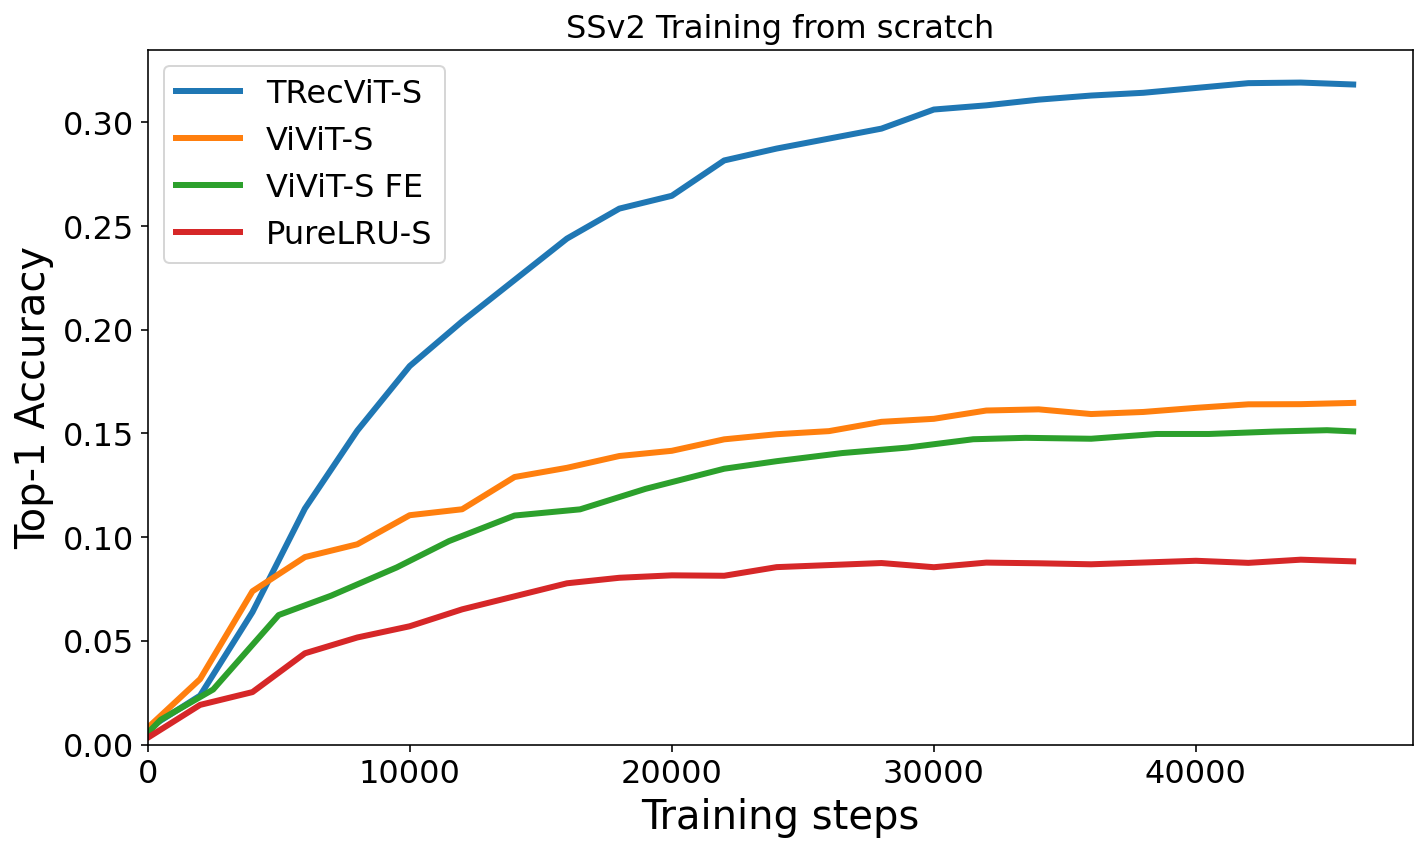
\includegraphics[width=.9\linewidth]{img/scratch.png}
  \caption{\ssm\ compared to baselines on supervised video classification on SSv2 dataset, trained from scratch. The plot shows the evolution of the evaluation accuracy as training progresses.
  }

  \label{fig:baselines}
\end{figure}
 

 \begin{figure*}[h]
  \centering
  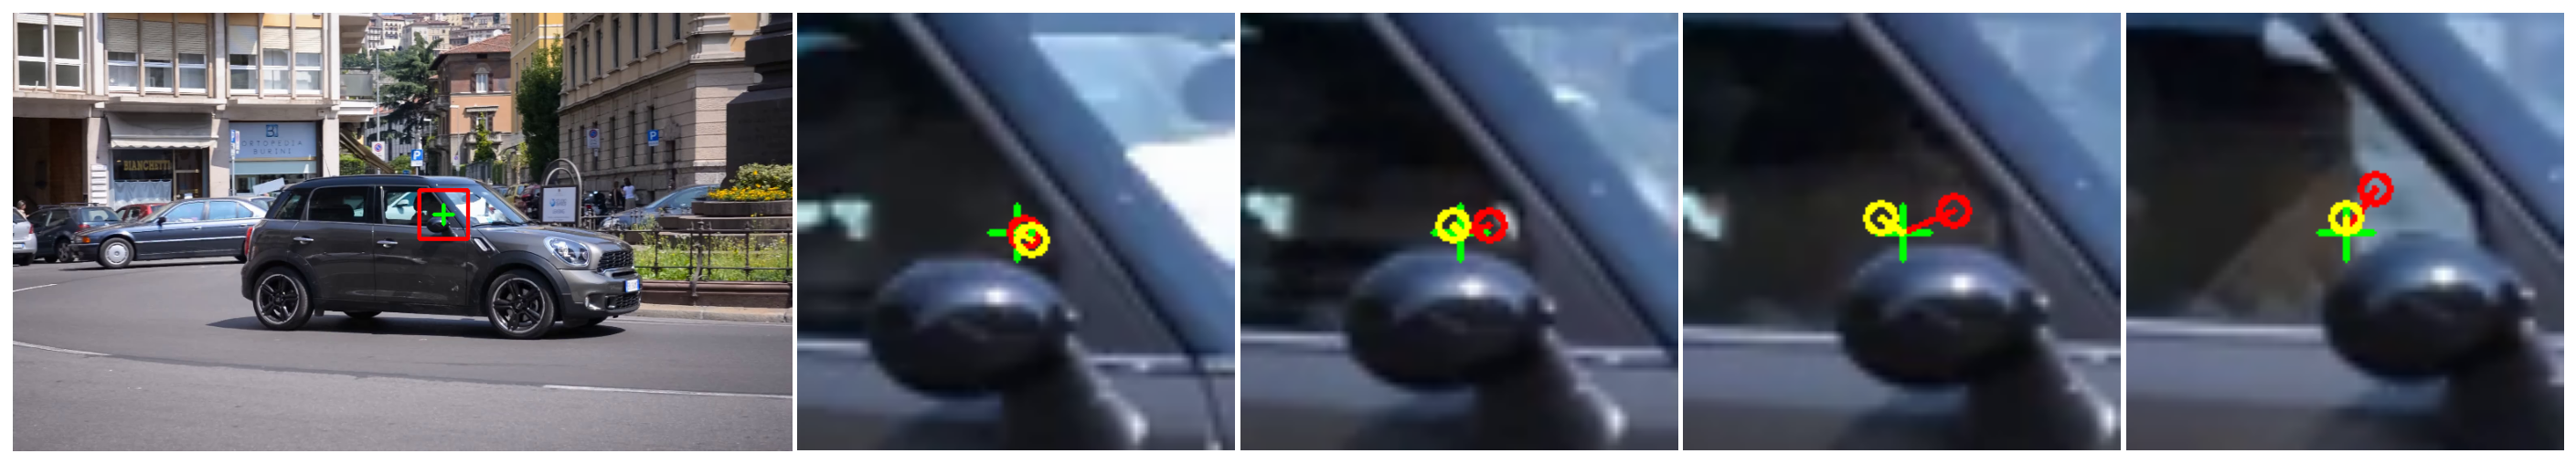
\includegraphics[width=\linewidth]{img/davis.png}
  \caption{Qualitative results obtained by \ssm\ for point tracking on DAVIS dataset compared to VideoMAE. The leftmost image indicates the point to track in the original frame, and the images towards the right show zoom-ins on subsequent frames. Green plus (+) marker indicates the ground truth, yellow circle indicates \ssm's predictions and red circles indicate VideoMAE's predictions.}
  \label{fig:tracking}
\end{figure*}


\begin{table}
    \centering
    \small{
    \begin{tabular}{l|c|c|r}
    \hline
    \textbf{Model} & \textbf{Patch size} & \textbf{Top-1 acc (\%)} & \textbf{\# params} \\
    \hline
    ViViT-B & (2, 16, 16) & 59.1 & 90M \\
    ViViT-L & (2, 16, 16) & 65.9 & 320M \\
    \ssm\ & (1, 16, 16) & \textbf{66.8} & 109M\\
    \hline
    \end{tabular}}
    \caption{Performance of \ssm\ compared to ViViT-B and ViViT-L baselines on SSv2 dataset with all models initialised from Imagenet pre-training. For ViViT-L, we use the result reported by its authors, for ViViT-B we obtained the results internally as they were not reported in the original paper for this dataset.}
    \label{tab:ssv2}
    \end{table}
    
\begin{table}
    \centering
    \small{
    \begin{tabular}{l|c|c|r}
    \hline
    \textbf{Model} & \textbf{Patch size} & \textbf{Top-1 acc (\%)} & \textbf{\# params} \\
    \hline
    ViViT-B & (2, 16, 16) & 78.1 & 90M \\
    ViViT-L & (2, 16, 16) & \textbf{78.7} & 320M \\
    \ssm\ & (1, 16, 16) & 78.4 & 109M\\
    \hline
    \end{tabular}}
    \caption{Performance of \ssm\ compared to ViViT-B and ViViT-L baselines on Kinetics400 dataset, with all models initialised from Imagenet pre-training. For ViViT-B and ViViT-L, we include the result we obtained internally by re-training the model on the current Kinetics400 dataset version; see footnote. In the original paper, the authors reported 80.3\% on Kinetics400 for ViViT-L.}
    \label{tab:kinetics}
    \end{table}

\subsection{Self-supervised masked autoencoding}
\label{sec:mae}
We use Kinetics400 for self-supervised pre-training from scratch and we report results on multiple downstream datasets and tasks by fine-tuning attention readout heads on top of frozen representations. We choose this setup, as opposed to fine-tuning end-to-end, as the  performance in this case more clearly reflects the quality of the pre-trained representations. As mentioned in the previous section, we use a large masking ratio (0.90), which makes pre-training very efficient. We report the number of parameters for every model considered. Note that the number of parameters for \ssm\ is different from the one reported in the previous section due to the addition of the readout heads.

\par \noindent \textbf{Video classification:}  We report video classification accuracy as downstream task using attention readout heads on SSv2 and Kinetics400. We compare the performance against VideoMAE-L~\cite{tong2022videomae} in Table~\ref{tab:selfsup}. Our model obtains slightly better performance on both datasets compared to this strong baseline, despite having almost 3$\times$ less parameters. 

\par \noindent \textbf{Point tracking:} To demonstrate that our model can handle dense(r) tasks as well, we evaluate the same frozen MAE representations for the point tracking task. We use the recurrent architecture in MooG~\cite{steenkiste2024moving} as a readout due to its simplicity. MooG uses light cross-attention layers to process the embeddings of each frame in order, and the readout state is carried over through time. We finetune the MooG readout head using MOVi-E dataset~\cite{movie} as done in popular point tracking works~\cite{DoerschYVG0ACZ23}. We evaluate these fine-tuned representations on two datasets: Perception Test~\citep{patraucean2023perception} and DAVIS dataset~\cite{davis2017} with point tracks extracted in~\cite{doersch2022tapvid}. We report average Jaccard metric~\cite{doersch2022tapvid} for \ssm\ compared with MooG and VideoMAE; see Table~\ref{tab:pt}. \ssm\ obtains better performance on both datasets compared to baselines, which reinforces the observation that our proposed model has strong motion modelling capabilities. We include qualitative results for this task in Figure~\ref{fig:tracking}. We can observe that the results are visibly better compared to VideoMAE. More visualisations are included in the supplementary material.

\begin{table}
    \centering
    \small{
    \begin{tabular}{l|c|c|r}
    \hline
    \textbf{Model} & \textbf{Dataset} & \textbf{Top-1 acc (\%)} & \textbf{\# params} \\
    \hline
    VideoMAE & Kinetics400 & 45.8 & 330M \\
    \ssm\ & Kinetics400 & \textbf{46.0} & 128M\\
    \hline
    \hline
    VideoMAE & SSv2 &  53.7 & 330M \\
    \ssm\ & SSv2 &  \textbf{53.9} & 128M\\
    \hline
    \end{tabular}}
    \caption{Performance of \ssm\ compared to VideoMAE on video classification using frozen MAE representations, pre-trained on Kinetics400.}
    \label{tab:selfsup}
    \end{table}

\begin{table}
    \centering
    \small{
    \begin{tabular}{l|c|c|c|r}
    \hline
    \textbf{Model} & \textbf{Dataset} & \textbf{\# frames} & \textbf{AJ} & \textbf{\# params} \\
    \hline
    MooG & DAVIS & 8 & 0.687 & 35M \\
    VideoMAE & DAVIS & 8 & 0.703 & 330M \\
    \ssm\ & DAVIS & 8 & \textbf{0.706} & 128M\\
    
    \hline
    \hline
    MooG & Perception Test & 16 & 0.760 & 46.5M \\
    VideoMAE & Perception Test & 16 & 0.761 & 330M \\
    \ssm\ & Perception Test & 16 & \textbf{0.783} & 128M\\
    \hline
    \end{tabular}}
    \caption{Performance of \ssm\ compared to baselines on point tracking task on DAVIS and Perception Test datasets. All models use frozen representations evaluated using the readout head from MooG.}
    \label{tab:pt}
    \end{table}

\begin{figure*}[h]
  \centering
  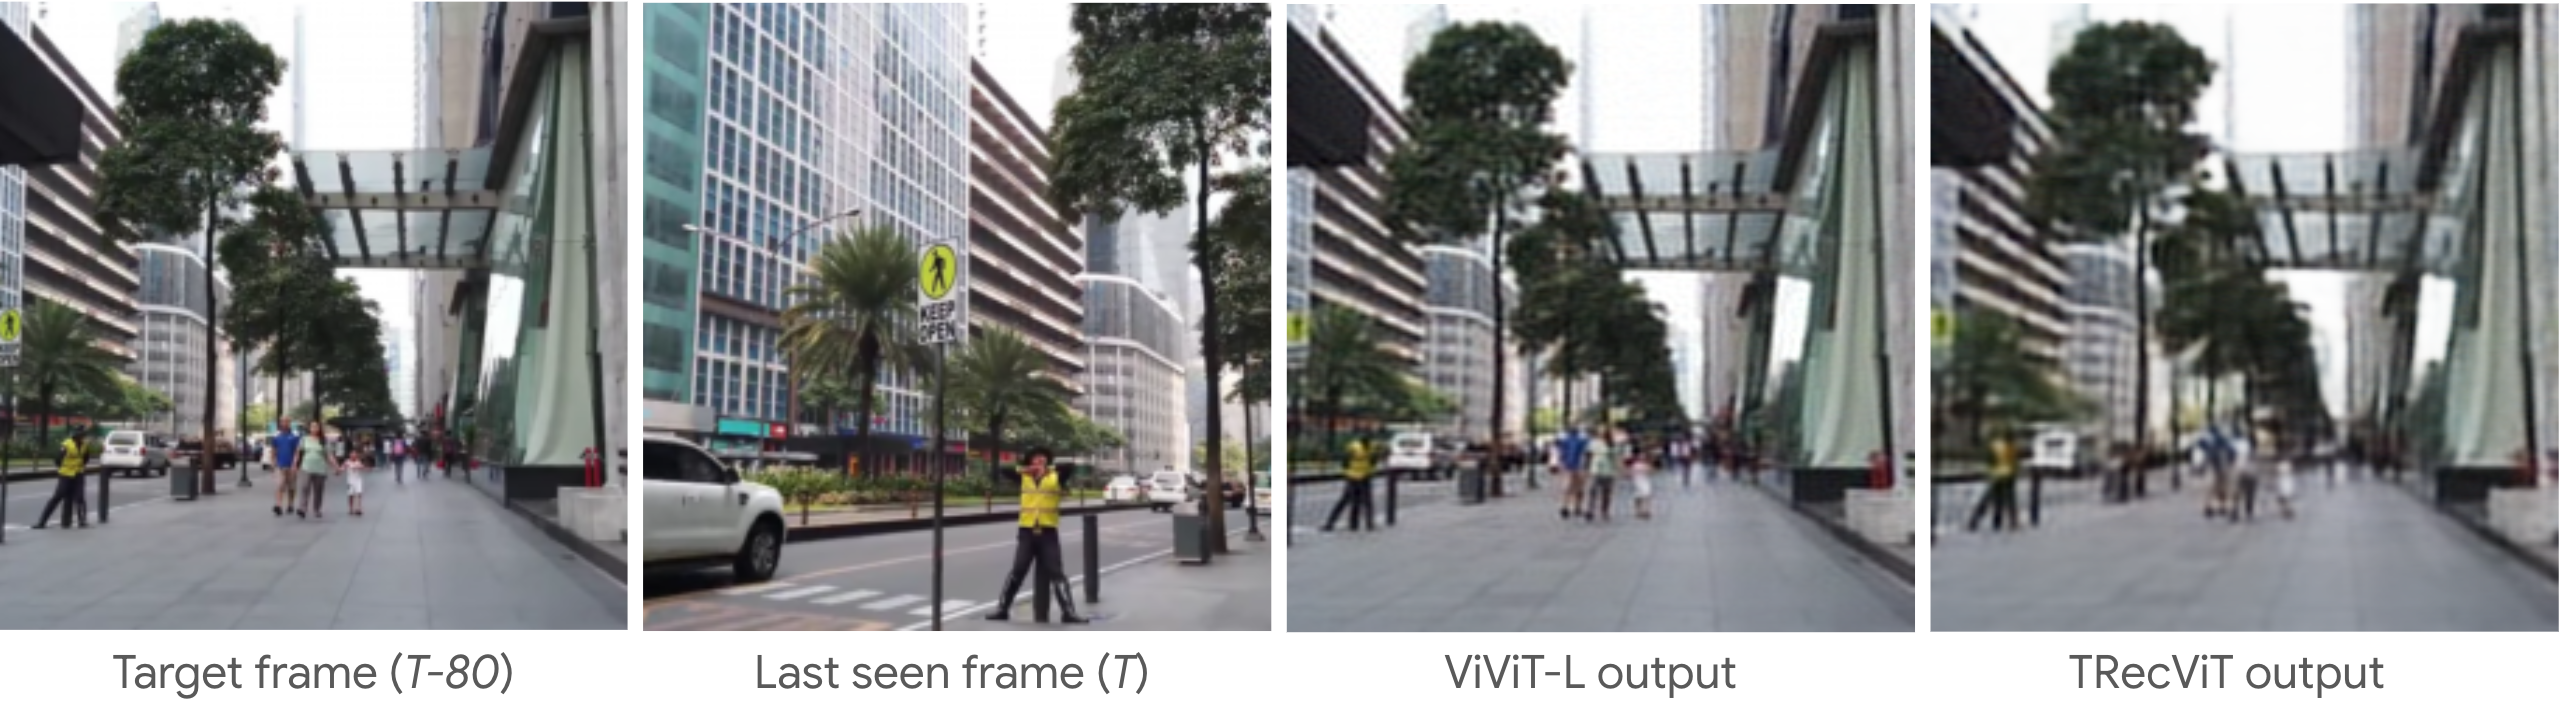
\includegraphics[width=\linewidth]{img/wtlong.png}
  \caption{Qualitative results obtained by \ssm\ on the dense memorisation task compared to ViViT-L. Both models are trained using Imagenet pre-trained weights, on video sequences of $T=64$ frames and they reconstruct the $(T-48)^\text{th}$ frame.}
  \label{fig:wt}
\end{figure*}

\begin{figure}[t]
\centering
\begin{subfigure}{0.48\linewidth}
    \centering
    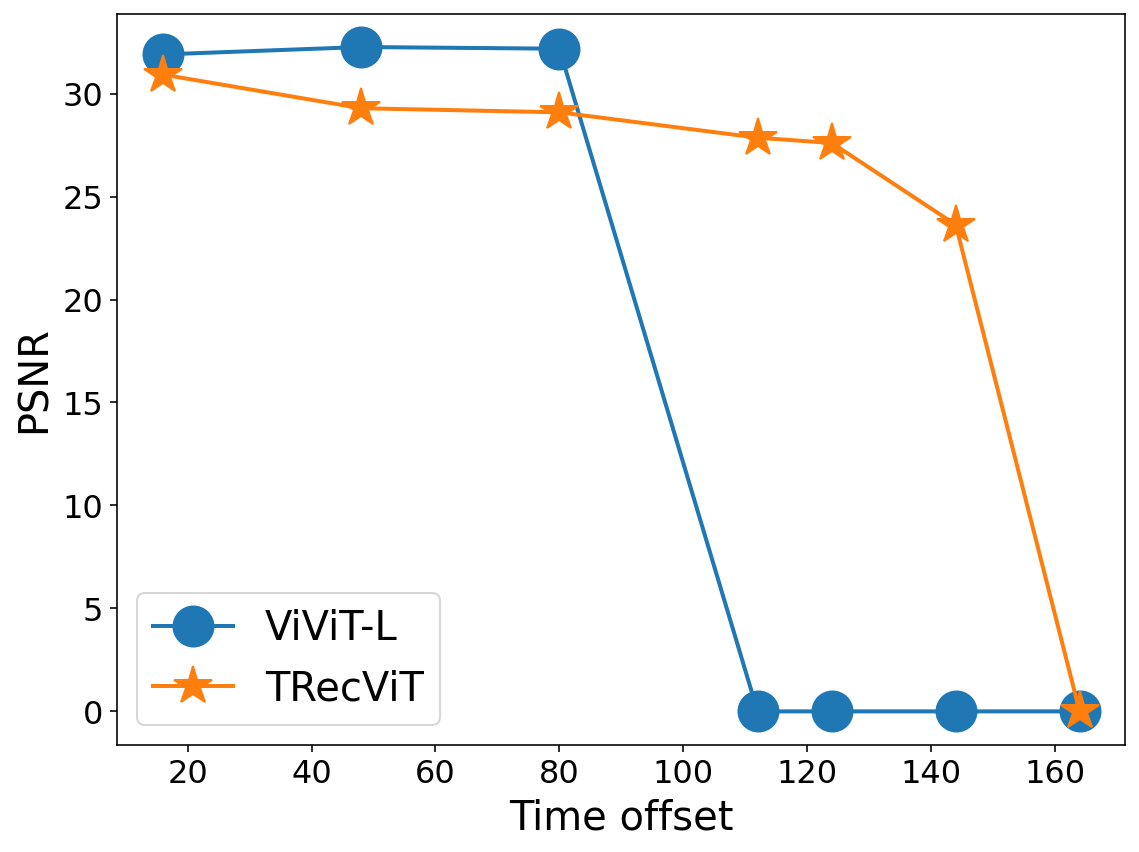
\includegraphics[width=\textwidth]{img/psnr.png}
    \caption{PSNR comparison}
\end{subfigure}%
\hfill
\begin{subfigure}{0.48\linewidth}
    \centering
    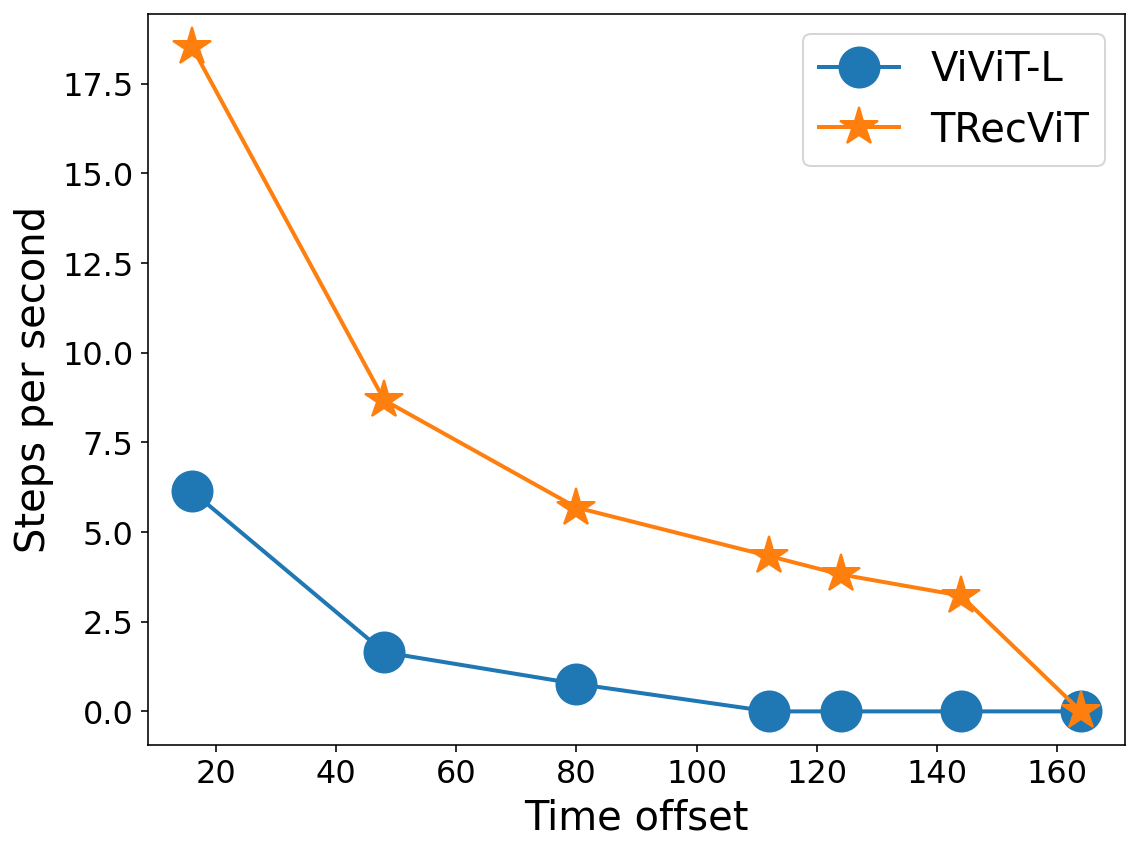
\includegraphics[width=\textwidth]{img/sps.png} 
    \caption{Steps-per-second comparison}
\end{subfigure}
\caption{Long video memorisation task. At time $T$, the model has to reconstruct the $(T-k)^\text{th}$ frame seen in the past. The plots show PSNR and throughput (steps-per-second) for increasing time offset $k$. For both models, the data points with $0$ value on the $y$-axis correspond to OOM.
}
\label{fig:psnr}
\end{figure}

\subsection{Long video memorisation task}
\label{sec:longtask}

Transformer models for language are known to be excellent at retrieving information from context, as they cache the keys and values for the entire history. On the other hand, LRUs / SSMs and RNNs in general struggle with such \emph{needle-in-the-haystack} style tasks as they need to perform the retrieval based on the compressed history kept in their recurrent state~\cite{jelassi2024repeat, de2024griffinmixinggatedlinear}. 
We are interested in studying this aspect in the video domain as well. We set up a simple reconstruction task where the model has to remember the frame seen at a given time-step in the past. For our analysis, we run multiple experiments where the model is tasked to reconstruct the $(T-k)^{\text{th}}$ frame from the past, with increasing value for $k\in\{16, 48, 80, 112, 144, 164\}$ frames. We employ Walking Tours dataset~\cite{venkataramanan2023imagenet}, which contains hour-long videos, and the scenery changes constantly, hence we are guaranteed that the video frames seen most recently will be very different compared to the frames seen earlier on. We scale the videos to $224\times224$ pixels. Again, we adopt ViViT-L as baseline, and we train both models using Imagenet pretrained weights. For ViViT-L, we keep all the outputs from all $T$ time steps and apply temporal pooling and a $1\times1$ convolution to get the expected shape for the reconstructed frame. For \ssm, we simply keep the output of the last layer at time step $T$ and reshape it to the expected shape. We show quantitative and qualitative results respectively in Figures~\ref{fig:psnr} and~\ref{fig:wt}. We can observe that there is a performance--efficiency trade-off at play for \ssm: its performance is slightly below ViViT's for shorter memory spans (16, 48, 80), but its efficiency (steps-per-second) is significantly higher. However, beyond 80 frames, ViViT-L goes out of memory, whilst \ssm\ continues to give decent results up to 144 frames, going out of memory towards 164 frames. Figure~\ref{fig:wt} shows qualitative results compared to the baseline for the case where the models have to remember the frame seen at $T-48$ in the past. We can observe that the quality of ViViT-L's reconstruction is good. For \ssm, whilst the overall structure (encoded in lower frequencies) is correct, it struggles to remember the high-frequency content of the image. This is to be expected due to the compression happening in the recurrent state of the model. However, given how different the last seen frame is from the target frame, we consider this to be a very promising result that warrants further investigation into the memorisation capabilities of our model, which we leave as future work.

\subsection{Generalisation to longer sequences}
\label{sec:gentask}

Using the same task as above, we analyse the generalisation capabilities to sequences longer than those used during training. Specifically, we train the models with sequences of length $T=64$ frames to reconstruct the $T-48$ frame, and evaluate them on longer sequences $T=96$ to reconstruct the same frame. The \ssm\ model can run on longer sequences without any modification. For the ViViT model, we need to adapt the positional encoding to accommodate longer sequences. We use interpolation to nearest neighbour to obtain the desired length; cubic interpolation led to worse results. The performance of \ssm\ degrades slightly, with PSNR going down from 29.3 (when evaluated on the same sequence length as in training $T=64$) to 26.4 when evaluated with $T=96$ frame sequences. ViViT's PSNR, however, drops significantly, from 32.3 when evaluated on the same sequence length, to 15.1 when evaluated on longer sequences. We include qualitative examples in Figure~\ref{fig:gentask} where we can observe that ViViT's output contains stronger artefacts compared to \ssm. 

\begin{figure}[h]
  \centering
  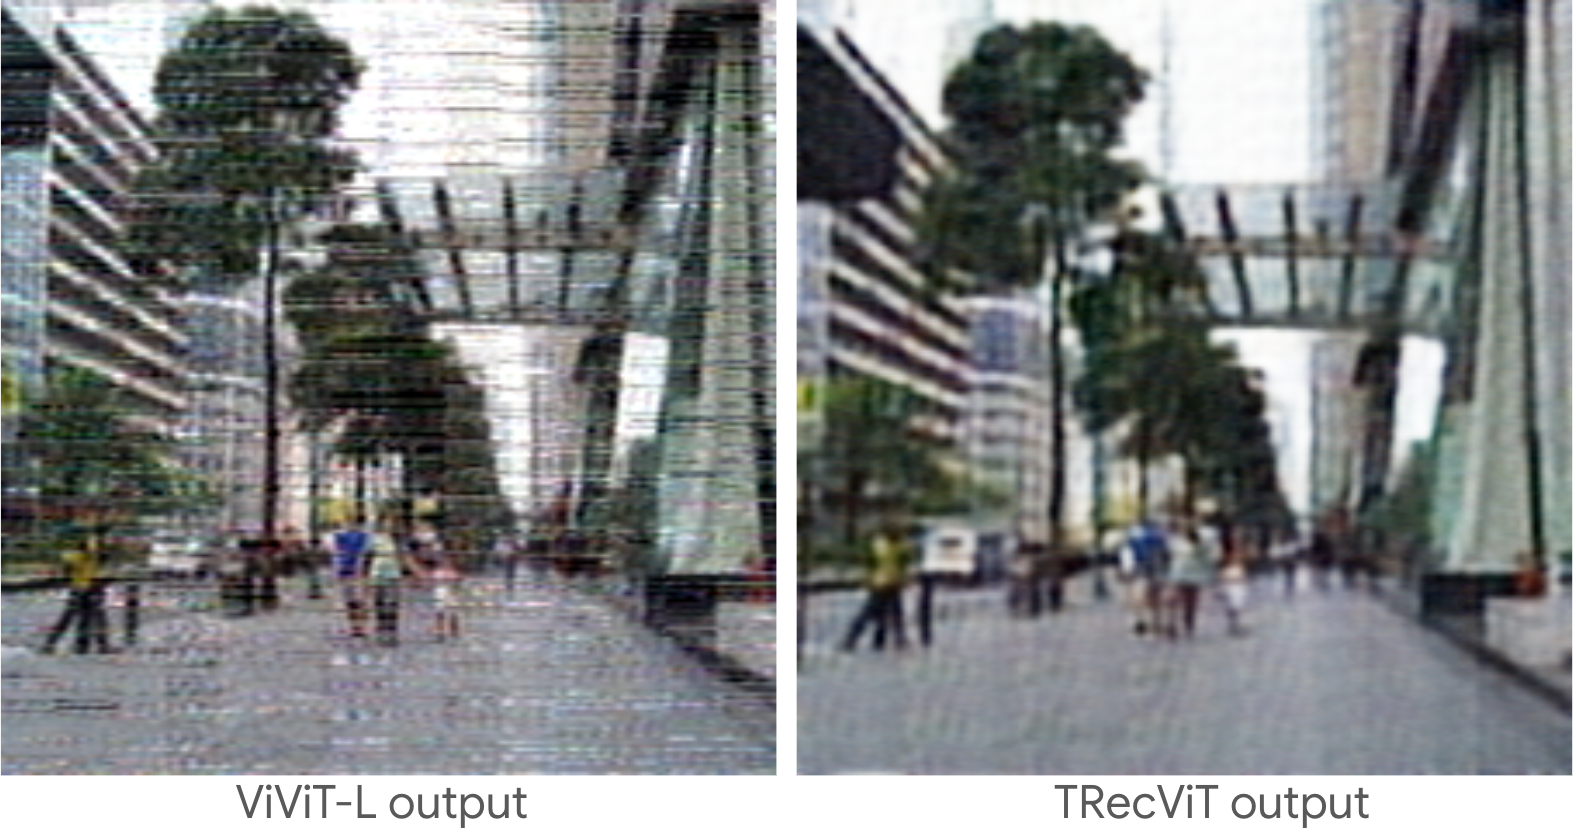
\includegraphics[width=\linewidth]{img/genlong.png}
  \caption{Generalisation to longer sequences. Both models are trained using Imagenet pre-trained weights, on video sequences of $T=64$ frames to reconstruct the $(T-48)^\text{th}$ frame; during evaluation, the models receive sequences of $T=96$ frames.}
  \label{fig:gentask}
\end{figure}

%
\section{Discussion and Conclusion}
%
In this work, we introduced an attention-free drop-in replacement to the core building block of many large-scale language models. ${\sf Hyena}$ operators are a recurrence of gating and implicitly parametrized long convolutions, can be evaluated efficiently in subquadratic time, and can learn in-context on very long sequences. 
%
On {\sc The Pile}, deep stacks of ${\sf Hyena}$ operators constitute one of the first attention-free, convolutional architectures to match perplexity and downstream performance of Transformers with a significant reduction in training compute. 
%
Our promising results at the sub-billion parameter scale suggest that attention may not be all we need, and that simpler subquadratic designs such as ${\sf Hyena}$, informed by a set of simple guiding principles and evaluation on mechanistic interpretability benchmarks, may form the basis for efficient large models. We are excited about what new capabilities {\sf Hyena} opens up as we scale and optimize the inference speed of these models.
\section*{Acknowledgments}

We would like to thank Karan Goel, Albert Gu, Avanika Narayan, Khaled Saab, Michael Zhang, Elliot Epstein and Sabri Eyuboglu for helpful discussion and feedback on earlier drafts, and Together Computer and Crusoe for providing the compute used to train models in this paper. We gratefully acknowledge the support of NIH under No. U54EB020405 (Mobilize), NSF under Nos. CCF1763315 (Beyond Sparsity), CCF1563078 (Volume to Velocity), and 1937301 (RTML); US DEVCOM ARL under No. W911NF-21-2-0251 (Interactive Human-AI Teaming); ONR under No. N000141712266 (Unifying Weak Supervision); ONR N00014-20-1-2480: Understanding and Applying Non-Euclidean Geometry in Machine Learning; N000142012275 (NEPTUNE); NXP, Xilinx, LETI-CEA, Intel, IBM, Microsoft, NEC, Toshiba, TSMC, ARM, Hitachi, BASF, Accenture, Ericsson, Qualcomm, Analog Devices, Google Cloud, Salesforce, Total, the HAI-GCP Cloud Credits for Research program,  the Stanford Data Science Initiative (SDSI), Department of Defense (DoD) through the National Defense Science and Engineering Graduate Fellowship (NDSEG) Program, and members of the Stanford DAWN project: Facebook, Google, and VMWare. This work is supported by NSF (1651565), AFOSR (FA95501910024), ARO (W911NF-21-1-0125), ONR, DOE (DE-SC0022222), CZ Biohub, and Sloan Fellowship. The U.S. Government is authorized to reproduce and distribute reprints for Governmental purposes notwithstanding any copyright notation thereon. Any opinions, findings, and conclusions or recommendations expressed in this material are those of the authors and do not necessarily reflect the views, policies, or endorsements, either expressed or implied, of NIH, ONR, or the U.S. Government. 

% % % bibliography
\bibliographystyle{abbrvnat}
\bibliography{_bibliography/main}
\clearpage
% % % appendix 
\appendix
%
\rule[0pt]{\columnwidth}{1pt}
\begin{center}
    \huge{Hyena Hierarchy} \\
    \vspace{0.3cm}
    \emph{Supplementary Material}
\end{center}
\rule[0pt]{\columnwidth}{1.5pt}
%
\doparttoc
\tableofcontents
%
\clearpage
\section{Experimental Details}
\label{appendix:experiment-details}
%
An implementation of ${\sf Hyena}$ can be found at \href{https://github.com/HazyResearch/safari}{this link}.
%

\subsection{Mechanistic Design Synthetic Benchmarks}\label{app:icl}
%
Our synthetic reasoning are inspired by mechanistic interpretability \citep{elhage2021mathematical}, \textit{in-context learning} (ICL) \citep{garg2022can} and language model benchmarking \citep{liang2022holistic} research. The evaluation revolves around $4$ main tasks:
\begin{itemize}[leftmargin=0.2in]
    \item \textbf{Associative recall:} Each string is produced by concatenating key-value tuples from a different random dictionary. This test verifies whether a model is able to extract right value given a key as prompt, effectively applying a data-controlled shift (delay).
    \item \textbf{Majority voting and counting:} Testing if a model can \textit{densely} activate its data-controlled matrix i.e., through many non-zero entries (consider the string '\textit{a a a a a a a a a a b} $\rightarrow$ \textit{a}').
    \item \textbf{ICL of linear functions:} Verifying whether a model can perform ICL on real-valued inputs. Prompts are generated as $x_1, w^k x_1, \dots, x_n \rightarrow w^k x_n$, where both $x_k$ and $w^k \in R^{n_o}$ are sampled from a normal distribution.  
    \item \textbf{Arithmetic:} Basic capability check. 
\end{itemize}

For each task, we train models using the hyperparameters shown in Table \ref{tab:synthetics}. We consider increasing settings of difficulty controlled by sequence length, spanning values $1024, 2048, 4098, 8196, 16392, 32784, 65568, 131136$ and vocabulary sizes $10, 20, 30, 40$. For ICL of functions, we vary instead the dimension $n_o$.

Note that for associative recall on longer sequences, multiple copies of key-value tuples appear in the prompt. To see this, consider how likely it is to sample multiple copies of a particular key-value pair with a vocabulary size of $40$, in order to form a sequence of $100$k characters. Models capable of looking further back in the sequence effectively see more data, and can solve challenging versions of the in-context learning task. Increasing the vocabulary size has the increasing the average distance between instances of the same key-value pair in each prompt, highlighting performance gaps between different approaches.

\begin{table}[ht]
    % \begin{minipage}[t]{0.4\linewidth}
      \small
      \caption{{(\bf Hyperparameter settings for reasoning and in-context learning tasks.)}.
      }
        \centering
        \begin{tabular}{lcc}
            \toprule
            Optimizer & AdamW \\
            Optimizer momentum & $\beta_1,\beta_2=0.9,0.98$ \\
            Base learning rate & 0.0005 \\
            Weight decay & 0.1 \\
            Dropout & None \\
            Batch size & 32 \\\
            Training epochs & 200 \\
            Num samples & 2000 \\ 
            Learning rate schedule & cosine decay \\
            Warmup epochs & 10 \\
            Warmup schedule & linear \\
            Number of layers & 2 \\ 
            Width & 64 \\
            \bottomrule
        \end{tabular}
        \label{tab:synthetics}
    % \end{minipage}
\end{table}

\paragraph{Long convolution comparisons:}
%
We compare different convolution parametrizations, embedding them in an order $2$ ${\sf Hyena}$ operator. All convolutions are applied separately to input channels (referred to as single-input single-output (SISO) in signal processing, or \textit{depthwise} in other machine learning contexts).

\begin{itemize}[leftmargin=0.1in]
    \item Conv1d: Explicit convolutions (regular convolution layers with fixed filter size). We use a fixed filter size of $64$, to match parameters of the other approaches.
    \item FNO: Filters parametrized explicitly in the frequency-domain \citep{li2020fourier}. We set the number of modes to $64$.
    \item H3: Implicit parametrization using state-space models (SSMs), and in particular the standard S4 \citep{gu2021efficiently}. We set the state dimension to $64$.
    \item TransferFunc: Implicit parametrization via transfer functions, a classical system-theoretic generalization of SSMs. Transfer functions are defined by a ratio of polynomials (we parametrize the coefficients, and evaluate the polynomials efficiently via FFTs). We set the order to $64$.
    \item CKConv: Implicit parametrization using {$\sf FFN$s} \citep{romero2021ckconv}. 
    \item item ${\sf Hyena}$: Combination of implicit parametrizations via {$\sf FFN$s} (with exponential decay modulation as shown in Figure \ref{fig:modul}), and short explicit filters.
\end{itemize}

CKConv and ${\sf Hyena}$ use the same size of ${\sf FFNs}$ (width $32$ to match in parameters).  
    
In Table \ref{synthetic2}, we report additional results on the challenging setting of sequence length $131072$ and vocabulary size $30$. Implicit parametrizations of convolutions outperform explicit parametrizations on associative recall, with CKConv and ${\sf Hyena}$ greatly improving on the ability to extract the right key, value relations from different inputs. In Appendix \ref{app:add_results}, we discuss how results on our synthetic tasks can be indicative of performance at a larger scale. 

%
\begin{table}[h]
\label{synthetic2}
\small
\centering
\vspace{-2mm}
\caption{Test accuracy (\%) in associative recall on sequences of length $131072$, vocabulary size $30$.}
\vspace{2mm}
\resizebox{0.45\linewidth}{!}
{
\setlength{\tabcolsep}{4pt}
\vspace{3em}
\begin{tabular}{@{}c|ccccccc@{}}
%\specialrule{.15em}{.05em}{.05em}
\toprule
${\sf Hyena}$ &\multicolumn{1}{c}{CKConv}&\multicolumn{1}{c}{TransferFunc} & \multicolumn{1}{c}{H3} & \multicolumn{1}{c} {FNO} & \multicolumn{1}{c}{Conv1d} \\
\midrule 
97.2 & 14.3 & 0.5 & 0.6 & 0.3 & 0.5 \\
\bottomrule
\end{tabular}
}
\end{table}
%

\paragraph{Operator comparisons:}
%
We compare different models on the same associative recall task, using hyperparameters in Table \ref{tab:synthetics}. ${\sf Hyena}$ uses our filter parametrization with decay windowing for long convolutions, and short explicit convolutions of size $3$ after the dense input projections. All other models use defaults from their largest scale experiment, while keeping the size to $2$ layers and width $64$.

\paragraph{A note on Transformer performance}
%
Transformers can solve associative recall tasks with longer sequences, provided the length does not prevent them from fitting in memory, and enough examples are present in the training data. In all our experiments, we keep the number of samples fixed ($2000$), a regime where Transformers struggle to find the generalizing solution (see Table \ref{synthetic2}).

For shorter sequences (see Appendix \ref{app:add_results}), Transformers solve the task easily even with limited data, comparably to {\sf Hyena}. 

More broadly, these different properties of attention and attention-free token-mixing layers may explain improved performance when they are combined in hybrid architectures \citep{dao2022hungry}. The focus on this work has been identifying an architecture capable of performing without attention, which is necessary to tackle domains where long sequences are common. However, when training with shorter sequences (up to $8$k), if final downstream performance is the only metric of interest, improved results can be obtained by hybridizing our models similarly to H3 \citep{dao2022hungry}.


%
\subsection{Language Modeling}
%
\paragraph{WikiText103:}
%
We train $125$M parameter models on {\sc WikiText103} and compare perplexity to Transformers, hybrid models such as H3 \citep{dao2022hungry}, and other variants of subquadratic attention. All models use the same GPT2 tokenizer with vocabulary size $50257$. We test order $3$ ${\sf Hyena}$ with our proposed filter parametrization for two long convolutions, and a shorter explicit convolution on the third. We also consider ${\sf Hyena}$ (slim) that are $1.5$x deeper than Transformers ($12$ versus $18$ layers), with width multiplier of the FFNs set to $2$. We find trading-off width for depth to be generally favourable. These modifications are made possible by the reduction in overall FLOPs of {\sf Hyena} operators compared to self-attention, in particular non-parametric FLOPs which include materialization of the attention matrix, application of softmax, and matrix-value reduction. 

\begin{table}[ht]
    % \begin{minipage}[t]{0.4\linewidth}
      \small
      \caption{Hyperparameter settings for {\sc The Pile}, $125$M).
      }
        \centering
        \begin{tabular}{lcc}
            \toprule
            Optimizer & AdamW \\
            Optimizer momentum & $\beta_1,\beta_2=0.9,0.98$ \\
            Peak learning rate & 0.0006 \\
            Warmup learning rate init & 0.000001 \\
            Learning rate min &  0.00006 \\ 
            % weight decay & \multicolumn{2}{c}{0.05} \\
            Weight decay & 0.1 \\
            Dropout & None \\
            Batch size & 256 \\
            % training epochs & \multicolumn{2}{c}{300} \\
            Learning rate schedule & cosine decay \\
            % warmup schedule & \multicolumn{2}{c}{linear} \\
            Warmup schedule & linear \\
            \bottomrule
        \end{tabular}
        \label{tab:pilehyper}
    % \end{minipage}
\end{table}

\paragraph{The Pile:}
%
We follow a same procedure and train $125$M and $355$M-sized models on {\sc The Pile} \citep{gao2020pile}. Hyperparameters are reported in Table \ref{tab:pilehyper}. Hyperparameters for $355$M are the same beyond a reduction in peak learning rate to $4\cdot 10^{-4}$. For larger models ($1.3$B), we set a learning rate of $2.2 \cdot 10^{-4}$.

We perform three experiments for each model type and size, and train for $5, 10, 15$ billion tokens at a sequence length $2024$ and global batch size $256$. All models are trained on a single node of $8$ $A100$ $80$GB GPUs. We use order $2$ ${\sf Hyena}$s, with the same architectural considerations described above for {\sc WikiText103}.
%
In addition to our data scaling experiments at $5$, $10$ and $15$ billion tokens, we provide preliminary results for models at the $1.3$B parameter scale ($10.8$ perplexity after $5$ billion tokens), and train a $153$M model ($130$ billion tokens), reaching a perplexity of $9.8$. The $153$M is the same used in our downstream evaluation on SuperGLUE. 

Training hyperparameters match those of standard GPT training pipelines, and are thus likely suboptimal for new attention-free architectures such as {\sf Hyena}. We run some preliminary experiments and find that e.g., some modifications to the learning rate schedule, currently involving linear warmup and cosine decay, to improve perplexity at convergence of {\sf Hyena} models (we recommend slightly lower learning rates for Hyena models compared to GPT of a similar size). Despite these findings, we use standard GPT hyperparameters for both GPT and {\sf Hyena}.
%
\paragraph{PG-19}

We also report results of additional training runs on other datasets. We train a ${\sf Hyena}$ $153$M model on the standard PG-19 long-range corpus \citep{raecompressive2019}, with a context length of $16$k tokens, reaching a test perplexity of $14.6$ (using the standard GPT2 tokenizer) in $8$ epochs.
%
\paragraph{Architectures}
%
Architectural hyperparameters for {\sf Hyena} are shown in Table \ref{hyena_arch}. We use sine as an activation function for the {\sf FFN} of {\sf Hyena} filters. 

\begin{table}[!bh]
\small
\centering
\caption{{\sf Hyena} architecture hyperparameters.}
\label{hyena_arch}
\setlength{\tabcolsep}{4pt}
\begin{tabular}{@{}c|cccccc@{}}
\toprule
Size & depth & width & {\sf FFN} width & filter {\sf FFN} width & filter {\sf FFN} depth & sine freq. \\
\midrule 
$125$M & $12$ & $768$ & $3072$ & $64$ & $4$ & $14$ \\ 
$125$M-slim &$18$ & $768$ & $1536$ & $64$ & $4$ & $14$\\ 
$153$M & $18$ & $864$ & $1728$ & $64$  & $4$ & $14$\\  
$355$M & $36$ & $1024$ & $2048$ & $64$ & $4$ & $14$ \\ 
$1.3$B & $36$ & $2048$ & $4096$ & $64$ & $4$ & $14$ \\ 
\bottomrule
\end{tabular}
\end{table}


\paragraph{FLOP computation}
%
The number of \textit{floating point operations} (FLOPs) reported in the main text are computed using the same strategy as in \citep{hoffmann2022training}. For GPT, we do not use the approximation, opting instead for the more accurate formula based on FLOP counts of individual layers. In the case of {\sf Hyena}, FLOPs are computed using the same method, except attention layers are replaced by:
\begin{itemize}
    \item[i.] Projections: order $\times$ d\_model $\times$ d\_model $\times$ seq\_len.
    \item[ii.] Short conv on projections: order $\times$ d\_model $\times$ seq\_len $\times$ filter\_len (usually $3$).
    \item[iii.] FFTConv: $5$ $\times$ (order - 1) $\times$ d\_model $\times$ $\log(\text{seq\_len})$
    $\times$ seq\_len.
    \item[iv.] Output: d\_model $\times$ d\_model $\times$ seq\_len.
\end{itemize}
with a leading factor $2$ to account for both additions and multiplications. 
%

\subsection{Downstream Evaluation}
%
\paragraph{SuperGLUE:} We evaluate models on the SuperGLUE \citep{wang2019superglue} with the parsing pipeline of \citep{arora2022ask}. For all tasks except WIC, CB and BoolQ, we generate a response using greedy decoding, then check for the gold label. WIC, CB and BoolQ use logit scoring instead of generation. 

\paragraph{Models}
The models considered are the open-source checkpoint of GPTNeo $125$M trained for $300$B tokens {\sc The Pile}, and the RWKV-v4 $169$M checkpoint trained for $332$B tokens on {\sc The Pile}. {\sf Hyena} is a $153$M model trained for $137$B tokens on {\sc The Pile}.
%
\paragraph{LAMBADA:} We evaluate ${\sf Hyena}$ on the LAMBADA \citep{paperno2016lambada} task. We apply a stop word filter and check whether predictions for all tokens corresponding to the last word agree with the ground truth. The small ${\sf Hyena}$ model trained on $137$B tokens reaches $44.64\%$ accuracy. 

\subsection{Image Classification}
\label{appendix:image-classification}

\paragraph
a{ImageNet:} We use ImageNet-1k which consists of 1000 classes and 1.3M images and train from scratch with no outside data on 8 Nvidia A100 GPUs. In our ViT benchmark, we swap the attention layers with the Hyena operator defined in our language experiments, and remove the class token and positional embeddings, similar to S4ND \citep{nguyen2022s4nd}. The parameter count is kept similar at 87M ViT-B (base) vs 88M Hyena-ViT. The training procedure from T2T-ViT \citep{yuan2021tokens} is used, including augmentations such as RandAugment \citep{cubuk2020randaugment}, Mixup \citep{zhang2017mixup}, and AugMix \citep{hendrycks2019augmix}. See table \ref{tab:imagenet_hparams} for hyperparameter settings used.

\paragraph{CIFAR-10:} We use CIFAR-10 in sequential and 2D experiments. For sequential, we use the Hyena operator defined in our language tasks and compare with an S4 model \citep{gu2021efficiently} of the same size by swapping layers in the residual blocks. In 2D, we learn Hyena filters (in both $x$ and $y$ dimensions) that are equal to the size of the input shape, and forgo the gating mechanism from our language experiments. We window (i.e., apply a soft mask spatially to) the Hyena filters with a decay term. The rate of decay varies across channels, ensuring different sizes of the filters at initialization. We compare with another implicit 2D convolution, S4ND \citep{nguyen2022s4nd}, by swapping the model layers with the 2D Hyena filters. The "isometric" model consists of 4 residual blocks of model dimension 128. We use basic image augmentations, 0.1 dropout, 0.03 weight decay and train for 100 epochs using a Nvidia T4 GPU.

\begin{table}[ht]
    % \begin{minipage}[t]{0.4\linewidth}
      \small
      \caption{ViT and ViT-Hyena settings for ImageNet-1k).
      }
        \centering
        \begin{tabular}{lcc}
            \toprule
            Image size & $224^2$ \\
            % image size & \multicolumn{2}{c}{$224^2$} \\
            Optimizer & AdamW \\
            % optimizer & \multicolumn{2}{c}{\textsc{AdamW}} \\
            % optimizer momentum & \multicolumn{2}{c}{$\beta_1,\beta_2=0.9,0.999$} \\
            Optimizer momentum & $\beta_1,\beta_2=0.9,0.999$ \\
            Weight init & trunc. normal (std=0.02) \\
            ViT base learning rate & $1e^{-3}$ \\
            Hyena-ViT base learning rate & $2e^{-4}$ \\
            % weight decay & \multicolumn{2}{c}{0.05} \\
            ViT weight decay & 0.05 \\
            Hyena-ViT weight decay & 0.01 \\
            Dropout & None \\
            Batch size & 1024 \\
            % training epochs & \multicolumn{2}{c}{300} \\
            Training epochs & 300 \\
            % learning rate schedule & \multicolumn{2}{c}{cosine decay} \\
            Learning rate schedule & cosine decay \\
            Warmup epochs & 10 \\
            % warmup schedule & \multicolumn{2}{c}{linear} \\
            Warmup schedule & linear \\
            Randaugment \citep{cubuk2020randaugment} & (9,0.5,layers=2)  \\
            Mixup \citep{zhang2017mixup} & 0.8 \\
            Cutmix \citep{yun2019cutmix} & 1.0 \\
            Random erasing \citep{zhong2020random} & 0.25 \\
            Label smoothing \citep{szegedy2016rethinking} & 0.1 \\
            Stochastic depth \citep{huang2016deep} & 0.1 \\
            Exp.mov. avg (EMA) \citep{polyak1992ema} & None \\
            \bottomrule
        \end{tabular}
        \label{tab:imagenet_hparams}
\end{table}
%




\section{Theoretical Results and Details}
%
\subsection{Proofs}
%
\paragraph{Proof of Proposition \ref{prop:causality}}
\proof A discrete $L$-by-$L$ operator is causal if it is lower triangular, i.e., when there is no leakage of future input information to the output. The ${\sf Hyena}$ operator $\sH$ is the product of alternating diagonal and Toeplitz matrices. Thus, if all the Toeplitz matrices $\sS_h^n$ are lower triangular then $\sH$ is lower triangular. In turn, each $\sS_h^n$ is lower triangular if and only if the filter $h$ is causal, concluding the proof. 
\endproof
%
\subsection{Analysis of Data-Controlled Mechanisms}\label{app:surrogate_att}
%
 We discuss the surrogate attention mechanism of {\sf Hyena}-$2$: $q,k,v\mapsto y$:
%
\begin{equation}\label{eq:linear_attention}
    \begin{aligned}
        z_t &= k_t(\varphi * v)_t \\
        y_t &= q_t(\psi * z)_t
    \end{aligned}
\end{equation}
%
If $\varphi$ and $\psi$ are convolutions parametrized via state-space models (SSMs), the above resembles the H3 mechanism \citep{dao2022hungry}. We investigate the effect of the convolutional kernels $\varphi$ and $\psi$ on the attention layer. We start by introducing a matrix representation of the layer, and we isolate the \textit{attention matrix} $\sA_\varphi^\psi(q,k)$ such that
%
\begin{equation}\label{eq:linear_attention_matrix}
    \begin{aligned}
        y &= \sA_\varphi^\psi(q,k)v.
    \end{aligned}
\end{equation}
%
\paragraph{Isolating the surrogate attention matrix}
%
In the case of length-$L$ discrete sequences%, the convolutions become sums, and we can rewrite \eqref{eq:linear_attention_convolution2} as
%
\begin{equation}\label{eq:linear_attention_convolution3}
    \begin{aligned}
        z_t &= k_t \sum_{m=0}^{L-1} \varphi_{t-m} v_m \\
        y_t &= q_t \sum_{m=0}^{L-1} \psi_{t-m} z_m\\
    \end{aligned}
\end{equation}
%
Therefore we can rewrite \eqref{eq:linear_attention} as
%
\begin{equation}
    \begin{aligned}
        y_t &= q_t \sum_{m=0}^{L-1} \psi_{t-m} k_m \sum_{n=0}^{L-1} \varphi_{m-n} v_n\\
             &= q_t \sum_{m=0}^{L-1} \sum_{n=0}^{L-1} \psi_{t-m} k_m \varphi_{m-n} v_n &&\quad\text{Move $\psi$, $k$ inside inner sum}\\
             &= q_t \sum_{n=0}^{L-1} \sum_{m=0}^{L-1} \psi_{t-m} k_m \varphi_{m-n} v_n &&\quad\text{Index shift}\\
             &= \sum_{n=0}^{L-1} q_t \sum_{m=0}^{L-1} \psi_{t-m} k_{m} \varphi_{m-n} v_{n}\\
    \end{aligned}
\end{equation}
%
And we can define the surrogate attention matrix $\sA_\varphi^\psi(q,k)$
%
\begin{equation}\label{eq:linear_attention_matrix2}
    \begin{aligned}
        [\sA_\varphi^\psi(q,k))]_{t,t'} &= q_t \sum_{m=0}^{L-1} \psi_{t-m} k_{m} \varphi_{m - t'}. \\
    \end{aligned}
\end{equation}
%
\begin{tcolorbox}[enhanced, drop fuzzy shadow, breakable, frame hidden, sharp corners] {\bf Continuous Signals:} 
    We can also consider the case of continuous signals on a group $G$. In the continuous case, we can expand the convolutions in \eqref{eq:linear_attention} as
    %
    \begin{equation}\label{eq:linear_attention_convolution}
        \begin{aligned}
            (\varphi * v)_t = \int_G \varphi_{t-g} v_g \dd g,\qquad
            (\psi * z)_t = \int_G \psi_{t - g} z_g \dd g
        \end{aligned}
    \end{equation}
    %
    This allows us to rewrite \eqref{eq:linear_attention} as
    %
    \begin{equation}\label{eq:linear_attention_convolution2}
        \begin{aligned}
            y_t &= q_t(\psi * k(\varphi * v))_t \\
            &= q_t \int_G \psi_{t-g} \left[ k_g\int_G \varphi_{g - \tau} v_\tau \dd \tau \right] \dd g \\
            &= q_t \int_G \left[ \int_G \psi_{t-g} k_g \varphi_{g - \tau} v_\tau \dd \tau \right] \dd g\\
            &= q_t \int_G \left[ \int_G \psi_{t-g} k_g \varphi_{g - \tau} v_\tau \dd g \right] \dd \tau &&\quad\text{Variable swap}\\
            &= \int_G \left[ q_t \int_G \psi_{t-g} k_g \varphi_{g - \tau} v_\tau \dd g \right] \dd \tau &&\quad\text{Pull $q_t$ in $\tau $ integral}\\
            & = \int_G \left[ q_t \int_G \psi_{t-g} k_g \varphi_{g - \tau} \dd g \right] v_\tau \dd \tau &&\quad\text{Pull $v_\tau$ out of $g$ integral}.
        \end{aligned}
    \end{equation}
    %
    There is a linear operator $\cA: v \mapsto y=\cA v$ which we interpret as the surrogate attention operator. $\cA$ is conditioned on the \textit{query} $q$, \textit{key} $k$ and filters $\varphi$ and $\psi$, $\cA = \cA_{\varphi}^\psi(q,k)$. The kernel $\mathcal K$ of the operator is given by
    \begin{equation}
        \begin{aligned}
            \mathcal K(t,t') &= q_t\int_G \psi_{t-g} k_g \varphi_{g - t'} \dd g \\
        \end{aligned}
    \end{equation}
    % %
    % Then, we can rewrite \eqref{eq:linear_attention} as
    % %
    % \begin{equation}\label{eq:linear_attention_convolution2}
    %     \begin{aligned}
    %         y_t &= q_t(\psi * k_t(\varphi * v)_t)_t \\
    %         &= q_t \int \psi_{t-r} k_r\int \varphi_{r - s} v_s ds dr \\
    %         &= q_t \int\int \psi_{t-r} k_r \varphi_{r - s} v_s dr ds
    %     \end{aligned}
    % \end{equation}
    %
        %
\end{tcolorbox}
%
\paragraph{Operator decomposition of the surrogate attention matrix}
%
We can decompose the linear map $v\mapsto y;~ y = \sA_\varphi^\psi(q,k)v$ into a sequence of factors, each dependent on a projection of the input $\sA_\varphi^\psi(q,k) = \sA^\psi(q) \sA_\varphi(k)$. Let $\sD_q$ and $\sD_k$ be the $L$-by-$L$ diagonal matrices whose respective main diagonal entries are the respective entries of $q$ and $k$. Then, we have that
%
\begin{equation}\label{eq:linear_attention_matrix3}
    \begin{aligned}
        \sA^\psi(q) &= \sD_q \sS_\psi,\qquad \sD_q = \diag(q), \\
        \sA_\varphi(k) &= \sD_k\sS_\varphi,\qquad \sD_k = \diag(k).
    \end{aligned}
\end{equation}
%
The matrix has been decomposed into two terms $\sA^\psi(q)$ and $\sA_\varphi(k)$ constructed by multiplying the diagonal matrices $\sD_q$ and $\sD_k$ with the Toeplitz matrices $\sS_\psi$ and $\sS_\varphi$. $\sS_\psi$ and $\sS_\varphi$ are the kernels of the convolution operators with filter's impulse responses $\psi$ and $\varphi$ respectively. In the current applications of interest, $\psi$ and $\varphi$ are chosen to be causal, i.e. $\psi[t]=0 \text{ for } t<0$ and $\varphi[t]=0 \text{ for } t<0$. This results in $\sS_\psi$ and $\sS_\varphi$ to be lower triangular matrices 
%
\begin{equation}
    \sS_\psi = \begin{bmatrix}
        \psi_0 & 0 & \cdots & 0 \\
        \psi_1 & \psi_0 & \cdots & 0 \\
        \vdots & \ddots & \ddots & \vdots \\
        \psi_{L-1} & \psi_{L-2} & \cdots & \psi_0
    \end{bmatrix}, \qquad
    \sS_\varphi = \begin{bmatrix}
        \varphi_0 & 0 & \cdots & 0 \\
        \varphi_1 & \varphi_0 & \cdots & 0 \\
        \vdots & \ddots & \ddots & \vdots \\
        \varphi_{L-1} & \varphi_{L-2} & \cdots & \varphi_0
    \end{bmatrix}.
\end{equation}
%
The surrogate attention matrix is then given by
%
\begin{equation}
    \sA_\varphi^\psi(q,k) = \sD_q \sS_\psi \sD_k \sS_\varphi
\end{equation}
%
We can expand the matrix multiplications in \eqref{eq:linear_attention_matrix3} in the case of causal filters $\varphi$ and $\psi$ as
%
\begin{equation}\label{eq:linear_attention_matrix4}
    \begin{aligned}
        \underset{ 
        \begin{bmatrix}
            q_0 &  &  &  \\
             & q_1 &  &  \\
             &  & \ddots &\\
             &  &  & q_{L-1}
        \end{bmatrix}}{\displaystyle \sD_q}
        %
        \underset{ 
        \begin{bmatrix}
            \psi_0 & & &  \\
            \psi_1 & \psi_0 & &  \\
            \vdots & \ddots & \ddots & \\
            \psi_{L-1} & \psi_{L-2} & \cdots & \psi_0
        \end{bmatrix}}{\displaystyle \sS_\psi}
        %
        \underset{ 
        \begin{bmatrix}
            k_0 &  &  &  \\
             & k_1 &  &  \\
             &  & \ddots &\\
             &  &  & k_{L-1}
        \end{bmatrix}}{\displaystyle \sD_k}
        %
        \underset{
        \begin{bmatrix}
            \varphi_0 & & &  \\
            \varphi_1 & \varphi_0 & &  \\
            \vdots & \ddots & \ddots & \\
            \varphi_{L-1} & \varphi_{L-2} & \cdots & \varphi_0
        \end{bmatrix}}{\displaystyle \sS_\varphi} 
        %
        &\\
        %
        \underset{\displaystyle \sA_\psi(q)}{ 
        = \begin{bmatrix}
            q_0 \psi_0 &  &  &  \\
            q_1 \psi_1 & q_1 \psi_0 &  &  \\
            \vdots & \ddots & \ddots & \\
            q_{L-1} \psi_{L-1} & q_{L-1} \psi_{L-2} & \cdots & q_{L-1} \psi_0
        \end{bmatrix}}
        %
        \underset{\displaystyle \sA_\varphi(k)}{ 
        \begin{bmatrix}
            k_0 \varphi_0 &  &  &  \\
            k_1 \varphi_1 & k_1 \varphi_0 &  &  \\
            \vdots & \ddots & \ddots & \\
            k_{L-1} \varphi_{L-1} & k_{L-1} \varphi_{L-2} & \cdots & k_{L-1} \varphi_0
        \end{bmatrix}} &\\
        %
    \end{aligned}
\end{equation}
%
\begin{tcolorbox}[enhanced, breakable, frame hidden, drop fuzzy shadow, sharp corners] {\bf Fourier decomposition of convolution operators:} The kernels of the convolution operators $\sS_\psi$ and $\sS_\varphi$ are diagonalized by the Fourier transform matrix $\sW\in\bC^{L\times L},~ \sW_{nm} = z^{m}, ~ z = e^{j 2\pi n / L}$. The Fourier transform of the convolution operator $\sS_\psi$ is given by
%
\begin{equation}
    \sS_\psi = \sW^* \sD_\Psi \sW, \quad \sS_\Phi = \sW^* \sD_\Phi \sW
\end{equation}
%
where $\sD_\Psi, \sD_\Phi\in\bC^{L\times L}$ are diagonal matrices constructed from the frequency responses (the \textit{discrete Fourier transform}) $\Psi=\sW\psi,\Phi=\sW\varphi$, respectively. This decomposition can be used to simplify the matrix multiplication in \eqref{eq:linear_attention_matrix4}:
%
\begin{equation}
    \sA = \sD_q \sS_\psi \sD_k \sS_\varphi = \sD_q  \sW^* \sD_\Psi \sW \sD_k \sW^* \sD_\Phi \sW
\end{equation}
%
An important property of the above is the non-commutativity of $\sD_q$ and $\sS_k$ with $\sW*$. If the two operators commuted, we would obtain
%
\begin{equation}
    \boxed{
    \sA =  \sD_q  \sW^* \sD_\Psi \sW \sD_k \sW^* \sD_\Phi \sW = \sW^* \sD_q \sD_\Psi \sD_k \sD_\Phi \sW
    }
\end{equation}
%
which reduces the entire layer to a simple convolution. The non-commutativity of the \textit{gating} term acts as a non-linearity in chain of convolution operators.
%
\end{tcolorbox}

%


%
\section{Discussion and Additional Results}\label{app:add_results}
%

\paragraph{Vocabulary size scaling}
%

Table \ref{scaling_vsize} showcases interesting correlation between associative recall performance for varying vocabulary sizes and loss on the {\sc The Pile}. In this case, we fix sequence length for associative recall to be $2048$, the same sequence length used to train all models on the {\sc The Pile}.

We observe a similar phenomenon on other slices of tasks from our mechanistic design benchmarks, indicating that it may be possible to derive predictive laws for performance at scale, based on fast experimentation on synthetic tasks with models of $1$ or $2$ layers. Surprisingly, performance on our language synthetics appears to be further linked to performance as attention replacement in other domains (Appendix \ref{appendix:image-classification} for results on image classification).

\begin{table}[!bh]
\small
\centering
\caption{{\sf Hyena} Accuracy on associative recall with varying vocabulary size $10$, $20$, $30$, $40$ in relation to test loss on {\sc The Pile} after $5$ billion tokens. We notice a correlation between the two performance metrics, suggesting that slices of our mechanistic design synthetics may be potentially predictive of performance at scale.}
\vspace{2mm}
\label{scaling_vsize}
\setlength{\tabcolsep}{4pt}
\begin{tabular}{@{}c|ccccc@{}}
\toprule
Model & Acc @ $10$ & Acc @ $20$ & Acc @ $30$ & Acc @ $40$ & Loss @ $5$B on {\sc The Pile} \\
\midrule 
Conv1d & $32$ & $11$ & $10$ & $8$ & $4.21$\\ 
AFT-conv & $55$ & $21$ & $12$ & $10$ & $3.57$\\ 
H3 & $92$ & $60$ & $13$ & $10$ & $2.69$\\
Transformer & $100$ & $100$ & $92$ & $82$ & $2.59$\\ 
{\sf Hyena} & $100$ & $100$ & $98$ & $85$ & $2.59$\\ 
\bottomrule
\end{tabular}
\end{table}

\paragraph{Single layer recall}
%

All experiments on our synthetic tasks default to $2$ layer models. We choose $2$ as it is the canonical number for mechanistic analysis of Transformers \citep{elhage2021mathematical} based on \textit{circuits}. Interestingly, a single layer of {\sf Hyena} (width $64$) is capable of performing associative recall, solving the task completely even in the challenging setting with vocabulary size $40$. Reverse engineering exactly how the single {\sf Hyena} operator is able to perform recall is left for future work.

\subsection{Learning Arithmetic}
%
We showcase an additional task in our mechanistic design benchmark: learning arithmetic. We train {\sf Hyena} models of increasing depth ($1$, $2$ and $3$ layers) on a dataset of $D_n$-digit addition. As an example, a $3$-digit addition input sample is given by the sequence
\[ 
    {\tt 1, 2, 3, 9, 5, 4, 1, 0, 7, 7}
\]
where the first $6$ digits contain the two $3$ digits numbers to add, and the last $4$ the result. Our models are optimized using standard autoregressive training i.e., predicting the next token, since they are causal. In particular, we optimize models to learn a map $x \mapsto y$ where $x$ is the original prompt without the last element, and $y$ equal to $x$ shifted right by one position. We mask the first $2 D_n - 1$ elements of the loss for each sequence since they contain predictions for addends and not results.

We report results in Figure \ref{fig:arithmetic}. A single layer of {\sf Hyena} is able to learn to perform addition with up to $4$ digits. Longer numbers require deeper models. In our experiments, alternative architectures such as AFT-conv struggle to learn arithmetic, signaling a cap in capability.

%
\begin{figure}
    \centering
    % This file was created with tikzplotlib v0.10.1.
\begin{tikzpicture}

\definecolor{darkgray176}{RGB}{176,176,176}
\definecolor{darkorange25512714}{RGB}{255,127,14}
\definecolor{steelblue31119180}{RGB}{31,119,180}
\definecolor{lightseagreen}{RGB}{32,178,170}

\begin{groupplot}[group style={group size=4 by 3, vertical sep=1.5cm}]
\nextgroupplot[
width=.28\linewidth,
xmin=0, xmax=80, ymin=0, ymax=3,
xlabel = {\sf \textit{epochs}}, xlabel style={at={(.5,-.12)}},
title={\sf \textbf{Layers}: 1, \textbf{Digits}: 2},
]
\addplot [line width=1.5pt, steelblue31119180]
table {%
0 19.8500556945801
1 14.6964349746704
2 7.82520723342896
3 3.55504679679871
4 2.27022767066956
5 1.65402841567993
6 1.01785886287689
7 0.558491230010986
8 0.368733167648315
9 0.291138887405396
10 0.211906835436821
11 0.187336325645447
12 0.170502096414566
13 0.157181560993195
14 0.158629402518272
15 0.142874717712402
16 0.142208084464073
17 0.14371845126152
18 0.145146876573563
19 0.151019930839539
20 0.142341703176498
21 0.1413953602314
22 0.142300367355347
23 0.13967701792717
24 0.139571860432625
25 0.145397439599037
26 0.142405033111572
27 0.151020094752312
28 0.1421257853508
29 0.14111365377903
30 0.143797650933266
31 0.14401076734066
32 0.142815381288528
33 0.142388001084328
34 0.142405718564987
35 0.144764810800552
36 0.143118128180504
37 0.142737194895744
38 0.14590784907341
39 0.142867088317871
40 0.144714966416359
41 0.141950070858002
42 0.144169852137566
43 0.142712444067001
44 0.142708286643028
45 0.144108429551125
46 0.143156096339226
47 0.143393129110336
48 0.144469887018204
49 0.143071204423904
50 0.144044503569603
51 0.144044890999794
52 0.143974304199219
53 0.144277423620224
54 0.143858775496483
55 0.144573271274567
56 0.144436970353127
57 0.143984705209732
58 0.144162073731422
59 0.144311249256134
60 0.144347608089447
61 0.144232347607613
62 0.14429560303688
63 0.144255951046944
64 0.144344061613083
65 0.144371554255486
66 0.144388929009438
67 0.144321799278259
68 0.144400626420975
69 0.144406169652939
70 0.144461944699287
71 0.144472315907478
72 0.144473671913147
73 0.144497185945511
74 0.14446847140789
75 0.144455879926682
76 0.144462257623672
77 0.144465088844299
78 0.144458100199699
79 0.144457831978798
};
\addplot [line width=1.5pt, lightseagreen]
table {%
0 0.028666665777564
1 0.116333335638046
2 0.209999993443489
3 0.416666656732559
4 0.523333311080933
5 0.628666639328003
6 0.761333346366882
7 0.86433333158493
8 0.906000018119812
9 0.934666633605957
10 0.950999975204468
11 0.957666635513306
12 0.960666656494141
13 0.966333329677582
14 0.967000007629395
15 0.968333303928375
16 0.968333303928375
17 0.972000002861023
18 0.970666646957397
19 0.969333350658417
20 0.97133332490921
21 0.969999969005585
22 0.97133332490921
23 0.970333337783813
24 0.972000002861023
25 0.970666646957397
26 0.971666634082794
27 0.968333303928375
28 0.969333350658417
29 0.968666672706604
30 0.967999994754791
31 0.969333350658417
32 0.969999969005585
33 0.970333337783813
34 0.969666659832001
35 0.969999969005585
36 0.969333350658417
37 0.968999981880188
38 0.970333337783813
39 0.968666672706604
40 0.969333350658417
41 0.968666672706604
42 0.969666659832001
43 0.968666672706604
44 0.968666672706604
45 0.969999969005585
46 0.968666672706604
47 0.968999981880188
48 0.968666672706604
49 0.969333350658417
50 0.969333350658417
51 0.968666672706604
52 0.968999981880188
53 0.968999981880188
54 0.968999981880188
55 0.969333350658417
56 0.969333350658417
57 0.969666659832001
58 0.969333350658417
59 0.969333350658417
60 0.969333350658417
61 0.969666659832001
62 0.969333350658417
63 0.969333350658417
64 0.969333350658417
65 0.969333350658417
66 0.969666659832001
67 0.969666659832001
68 0.969666659832001
69 0.969333350658417
70 0.969666659832001
71 0.969333350658417
72 0.969666659832001
73 0.969666659832001
74 0.969666659832001
75 0.969666659832001
76 0.969666659832001
77 0.969666659832001
78 0.969666659832001
79 0.969666659832001
};

\nextgroupplot[
width=.28\linewidth,
xmin=0, xmax=80, ymin=0, ymax=3,
xlabel = {\sf \textit{epochs}}, xlabel style={at={(.5,-.12)}},
title={\sf \textbf{Layers}: 1, \textbf{Digits}: 4},
]
\addplot [line width=1.5pt, steelblue31119180]
table {%
0 16.1500988006592
1 9.3095645904541
2 3.06095433235168
3 2.60867929458618
4 2.55007100105286
5 2.50773167610168
6 2.52670645713806
7 2.44119143486023
8 2.40223932266235
9 2.35879063606262
10 2.25714492797852
11 1.98748922348022
12 1.27430593967438
13 0.938567161560059
14 0.772136270999908
15 0.638410925865173
16 0.570026755332947
17 0.490775108337402
18 0.459385335445404
19 0.434654980897903
20 0.412004470825195
21 0.400936722755432
22 0.398127645254135
23 0.388456076383591
24 0.388161569833755
25 0.385582119226456
26 0.374141991138458
27 0.384999603033066
28 0.38512659072876
29 0.378220170736313
30 0.386807471513748
31 0.384234815835953
32 0.391106456518173
33 0.385352909564972
34 0.390837848186493
35 0.390760451555252
36 0.390821188688278
37 0.400349467992783
38 0.416233658790588
39 0.420717358589172
40 0.406466692686081
41 0.421025425195694
42 0.426708698272705
43 0.433257818222046
44 0.431459188461304
45 0.43684259057045
46 0.444573581218719
47 0.434202462434769
48 0.442012399435043
49 0.452698796987534
50 0.462604761123657
51 0.459520161151886
52 0.474672704935074
53 0.471127927303314
54 0.475456863641739
55 0.476716458797455
56 0.478782892227173
57 0.484319865703583
58 0.484086513519287
59 0.494138330221176
60 0.495136737823486
61 0.496272444725037
62 0.501498639583588
63 0.502588450908661
64 0.50678962469101
65 0.50735992193222
66 0.509675145149231
67 0.510948896408081
68 0.514151930809021
69 0.513838350772858
70 0.514931380748749
71 0.515583395957947
72 0.516949594020844
73 0.517191410064697
74 0.517659068107605
75 0.517891824245453
76 0.518097937107086
77 0.518251657485962
78 0.518297016620636
79 0.518313884735107
};
\addplot [line width=1.5pt, lightseagreen]
table {%
0 0.0529999993741512
1 0.0975999981164932
2 0.191399991512299
3 0.229999989271164
4 0.242399990558624
5 0.252000004053116
6 0.24719999730587
7 0.269600003957748
8 0.279799997806549
9 0.285600006580353
10 0.308999985456467
11 0.376199990510941
12 0.55919998884201
13 0.674799978733063
14 0.730799973011017
15 0.783399999141693
16 0.812399983406067
17 0.844799995422363
18 0.85099995136261
19 0.864799976348877
20 0.870199978351593
21 0.879399955272675
22 0.875
23 0.875400006771088
24 0.875400006771088
25 0.878799974918365
26 0.883599996566772
27 0.882599949836731
28 0.883199989795685
29 0.885199964046478
30 0.884999990463257
31 0.880799949169159
32 0.883599996566772
33 0.881599962711334
34 0.878799974918365
35 0.882799983024597
36 0.880999982357025
37 0.874799966812134
38 0.879399955272675
39 0.873999953269958
40 0.879199981689453
41 0.879599988460541
42 0.876599967479706
43 0.870199978351593
44 0.875999987125397
45 0.872199952602386
46 0.873199999332428
47 0.875
48 0.872999966144562
49 0.872399985790253
50 0.869799971580505
51 0.871800005435944
52 0.867799997329712
53 0.869599997997284
54 0.871399998664856
55 0.872199952602386
56 0.870599985122681
57 0.869799971580505
58 0.870799958705902
59 0.871399998664856
60 0.86899995803833
61 0.867999970912933
62 0.868399977684021
63 0.86899995803833
64 0.868599951267242
65 0.867199957370758
66 0.867399990558624
67 0.866400003433228
68 0.866400003433228
69 0.86679995059967
70 0.866599977016449
71 0.866199970245361
72 0.864999949932098
73 0.864999949932098
74 0.865799963474274
75 0.86599999666214
76 0.86599999666214
77 0.865799963474274
78 0.86599999666214
79 0.86599999666214
};

\nextgroupplot[
width=.28\linewidth,
xmin=0, xmax=80, ymin=0, ymax=3,
xlabel = {\sf \textit{epochs}}, xlabel style={at={(.5,-.12)}},
title={\sf \textbf{Layers}: 1, \textbf{Digits}: 8},
]
\addplot [line width=1.5pt, steelblue31119180]
table {%
0 14.3578033447266
1 3.8737359046936
2 2.54545974731445
3 2.48529529571533
4 2.47089076042175
5 2.46856355667114
6 2.45537662506104
7 2.44946837425232
8 2.44510650634766
9 2.41553831100464
10 2.43618893623352
11 2.40809869766235
12 2.40338063240051
13 2.37879395484924
14 2.38422560691833
15 2.38212370872498
16 2.37861776351929
17 2.37318658828735
18 2.36681127548218
19 2.35814833641052
20 2.36178827285767
21 2.361496925354
22 2.36390781402588
23 2.38373208045959
24 2.35792994499207
25 2.3693311214447
26 2.35754632949829
27 2.36197781562805
28 2.36152505874634
29 2.35618710517883
30 2.35922265052795
31 2.36109733581543
32 2.36173009872437
33 2.36683344841003
34 2.36295104026794
35 2.3664882183075
36 2.36541700363159
37 2.37293648719788
38 2.36519360542297
39 2.38222622871399
40 2.37964797019958
41 2.36569762229919
42 2.37497329711914
43 2.37994503974915
44 2.37199425697327
45 2.37724566459656
46 2.38150119781494
47 2.38069629669189
48 2.38510227203369
49 2.38388133049011
50 2.38761973381042
51 2.38821506500244
52 2.38862228393555
53 2.39248323440552
54 2.38765239715576
55 2.38975262641907
56 2.39051580429077
57 2.39481663703918
58 2.3921046257019
59 2.39409875869751
60 2.3915376663208
61 2.40076923370361
62 2.40027952194214
63 2.40333604812622
64 2.3976948261261
65 2.39705681800842
66 2.40437078475952
67 2.40656232833862
68 2.40609264373779
69 2.40588068962097
70 2.4073007106781
71 2.40962290763855
72 2.40819454193115
73 2.40783739089966
74 2.40781116485596
75 2.40918469429016
76 2.40912628173828
77 2.40904855728149
78 2.40932416915894
79 2.40935015678406
};
\addplot [line width=1.5pt, lightseagreen]
table {%
0 0.0666666701436043
1 0.102111108601093
2 0.161111116409302
3 0.161888897418976
4 0.165444448590279
5 0.159111112356186
6 0.166999995708466
7 0.160222217440605
8 0.172333329916
9 0.166222229599953
10 0.165111109614372
11 0.162888884544373
12 0.177555561065674
13 0.18522222340107
14 0.182444453239441
15 0.178111106157303
16 0.187666669487953
17 0.183333337306976
18 0.189666673541069
19 0.184777781367302
20 0.179444447159767
21 0.182333335280418
22 0.179333329200745
23 0.181999996304512
24 0.184333339333534
25 0.17622222006321
26 0.183888897299767
27 0.183222219347954
28 0.178222224116325
29 0.180111110210419
30 0.177444443106651
31 0.182777777314186
32 0.18133333325386
33 0.181888893246651
34 0.179000005125999
35 0.179555550217628
36 0.180333331227303
37 0.177111119031906
38 0.180111110210419
39 0.182111114263535
40 0.179222226142883
41 0.181999996304512
42 0.182222217321396
43 0.17733334004879
44 0.182333335280418
45 0.176777780056
46 0.177777782082558
47 0.181444451212883
48 0.178333342075348
49 0.180222228169441
50 0.181888893246651
51 0.179888889193535
52 0.180333331227303
53 0.18577778339386
54 0.182777777314186
55 0.182666674256325
56 0.179555550217628
57 0.179666668176651
58 0.181444451212883
59 0.180444449186325
60 0.182444453239441
61 0.18077777326107
62 0.18077777326107
63 0.179222226142883
64 0.181777775287628
65 0.182666674256325
66 0.180111110210419
67 0.178333342075348
68 0.179000005125999
69 0.179444447159767
70 0.180000007152557
71 0.181555554270744
72 0.180555552244186
73 0.182888895273209
74 0.182555556297302
75 0.182333335280418
76 0.182111114263535
77 0.181888893246651
78 0.182222217321396
79 0.182222217321396
};

\nextgroupplot[
width=.28\linewidth,
xmin=0, xmax=80, ymin=0, ymax=3,
xlabel = {\sf \textit{epochs}}, xlabel style={at={(.5,-.12)}},
title={\sf \textbf{Layers}: 1, \textbf{Digits}: 16},
]
\addplot [line width=1.5pt, steelblue31119180]
table {%
0 13.3896608352661
1 2.4637393951416
2 2.41776585578918
3 2.41459488868713
4 2.41029858589172
5 2.40332818031311
6 2.39010691642761
7 2.38682103157043
8 2.36892580986023
9 2.37366390228271
10 2.35293793678284
11 2.3484034538269
12 2.34839034080505
13 2.35122561454773
14 2.33330297470093
15 2.32946991920471
16 2.32257032394409
17 2.31851387023926
18 2.32499313354492
19 2.32041049003601
20 2.31581830978394
21 2.31489753723145
22 2.31470918655396
23 2.31609439849854
24 2.32146263122559
25 2.31520509719849
26 2.31362748146057
27 2.31495547294617
28 2.31490302085876
29 2.31113910675049
30 2.31065988540649
31 2.30958938598633
32 2.3088047504425
33 2.30311727523804
34 2.29875183105469
35 2.28990006446838
36 2.28776574134827
37 2.29134130477905
38 2.28635406494141
39 2.27704215049744
40 2.2708911895752
41 2.28026819229126
42 2.26915049552917
43 2.26785373687744
44 2.28163981437683
45 2.25965714454651
46 2.25188446044922
47 2.24825119972229
48 2.24312520027161
49 2.26840877532959
50 2.27526140213013
51 2.24999070167542
52 2.24077796936035
53 2.2386109828949
54 2.23606657981873
55 2.24958920478821
56 2.23392534255981
57 2.24961733818054
58 2.22815680503845
59 2.226646900177
60 2.22495222091675
61 2.22468113899231
62 2.22432208061218
63 2.2222740650177
64 2.23156690597534
65 2.22099447250366
66 2.22111630439758
67 2.22076296806335
68 2.2199809551239
69 2.2192177772522
70 2.21828413009644
71 2.21872520446777
72 2.21836304664612
73 2.21803283691406
74 2.2178647518158
75 2.21793818473816
76 2.21792387962341
77 2.2178361415863
78 2.21782398223877
79 2.21782827377319
};
\addplot [line width=1.5pt, lightseagreen]
table {%
0 0.0714705884456635
1 0.11011765152216
2 0.132823526859283
3 0.129000008106232
4 0.130882352590561
5 0.133529409766197
6 0.130941182374954
7 0.128470584750175
8 0.130529418587685
9 0.134705886244774
10 0.134117648005486
11 0.137470588088036
12 0.134470596909523
13 0.144117653369904
14 0.142529413104057
15 0.145588234066963
16 0.144176468253136
17 0.143529415130615
18 0.143294125795364
19 0.144941180944443
20 0.144529417157173
21 0.146176472306252
22 0.145882353186607
23 0.144882351160049
24 0.141647055745125
25 0.147647067904472
26 0.143235296010971
27 0.147882357239723
28 0.145235300064087
29 0.146823525428772
30 0.143470585346222
31 0.147176474332809
32 0.151764705777168
33 0.151941180229187
34 0.155411764979362
35 0.157411769032478
36 0.151647061109543
37 0.157882362604141
38 0.16058823466301
39 0.161058828234673
40 0.164294123649597
41 0.16623529791832
42 0.162647068500519
43 0.165647059679031
44 0.165529415011406
45 0.170470595359802
46 0.167470589280128
47 0.170823529362679
48 0.172470599412918
49 0.171294122934341
50 0.16288235783577
51 0.173117652535439
52 0.176882356405258
53 0.176352947950363
54 0.175823539495468
55 0.172411769628525
56 0.178352952003479
57 0.174470588564873
58 0.17964705824852
59 0.180470585823059
60 0.183294117450714
61 0.180470585823059
62 0.181235298514366
63 0.18464706838131
64 0.178470596671104
65 0.182647064328194
66 0.181823536753654
67 0.181823536753654
68 0.183294117450714
69 0.183882355690002
70 0.183352947235107
71 0.18299999833107
72 0.182882353663445
73 0.182823538780212
74 0.182000011205673
75 0.182941183447838
76 0.182529419660568
77 0.183588236570358
78 0.183352947235107
79 0.183294117450714
};

\nextgroupplot[
width=.28\linewidth,
xmin=0, xmax=80, ymin=0, ymax=3,
xlabel = {\sf \textit{epochs}}, xlabel style={at={(.5,-.12)}},
title={\sf \textbf{Layers}: 2, \textbf{Digits}: 2},
]
\addplot [line width=1.5pt, steelblue31119180]
table {%
0 24.4404411315918
1 13.2875127792358
2 5.20647954940796
3 2.54925847053528
4 1.88095319271088
5 1.28719222545624
6 0.691513001918793
7 0.41288086771965
8 0.284831345081329
9 0.207248702645302
10 0.210182130336761
11 0.180913403630257
12 0.186495959758759
13 0.179402127861977
14 0.160388574004173
15 0.161240622401237
16 0.159042432904243
17 0.160917177796364
18 0.159058392047882
19 0.159014627337456
20 0.158749788999557
21 0.159613475203514
22 0.159566521644592
23 0.160102874040604
24 0.159766063094139
25 0.15918280184269
26 0.159575074911118
27 0.159866273403168
28 0.159521296620369
29 0.160297513008118
30 0.159569889307022
31 0.159797504544258
32 0.159519046545029
33 0.159697815775871
34 0.160033211112022
35 0.159811347723007
36 0.159069553017616
37 0.159974843263626
38 0.160136207938194
39 0.15976682305336
40 0.158891603350639
41 0.159282475709915
42 0.159819528460503
43 0.15903602540493
44 0.15924508869648
45 0.15905798971653
46 0.159362345933914
47 0.159403994679451
48 0.158938214182854
49 0.159000501036644
50 0.158628910779953
51 0.158906131982803
52 0.158887311816216
53 0.158724322915077
54 0.158732697367668
55 0.158863231539726
56 0.158664405345917
57 0.158806934952736
58 0.158759281039238
59 0.158662021160126
60 0.158840134739876
61 0.158669501543045
62 0.158548086881638
63 0.158624678850174
64 0.158582150936127
65 0.158590689301491
66 0.158621340990067
67 0.158656343817711
68 0.158537909388542
69 0.158517643809319
70 0.158494263887405
71 0.158518061041832
72 0.158539310097694
73 0.158509373664856
74 0.158506512641907
75 0.158517405390739
76 0.158509626984596
77 0.158510744571686
78 0.158514410257339
79 0.15851528942585
};
\addplot [line width=1.5pt, lightseagreen]
table {%
0 0.00533333327621222
1 0.110333330929279
2 0.285333335399628
3 0.434666663408279
4 0.541333317756653
5 0.68533331155777
6 0.825999975204468
7 0.898000001907349
8 0.931666672229767
9 0.954333305358887
10 0.956666648387909
11 0.960999965667725
12 0.962666630744934
13 0.960999965667725
14 0.970666646957397
15 0.967333316802979
16 0.968333303928375
17 0.967333316802979
18 0.965666651725769
19 0.966333329677582
20 0.967000007629395
21 0.967666685581207
22 0.967000007629395
23 0.967666685581207
24 0.967333316802979
25 0.967999994754791
26 0.967333316802979
27 0.967999994754791
28 0.968333303928375
29 0.968666672706604
30 0.969333350658417
31 0.969333350658417
32 0.969666659832001
33 0.968999981880188
34 0.969333350658417
35 0.969666659832001
36 0.969333350658417
37 0.969333350658417
38 0.968999981880188
39 0.969666659832001
40 0.970666646957397
41 0.969999969005585
42 0.969333350658417
43 0.969999969005585
44 0.969999969005585
45 0.969999969005585
46 0.969333350658417
47 0.969666659832001
48 0.969666659832001
49 0.969666659832001
50 0.969666659832001
51 0.969666659832001
52 0.969666659832001
53 0.969666659832001
54 0.969666659832001
55 0.969666659832001
56 0.969999969005585
57 0.969999969005585
58 0.969999969005585
59 0.969666659832001
60 0.969666659832001
61 0.969999969005585
62 0.969666659832001
63 0.969666659832001
64 0.969666659832001
65 0.969666659832001
66 0.969666659832001
67 0.969666659832001
68 0.969666659832001
69 0.969666659832001
70 0.969666659832001
71 0.969666659832001
72 0.969666659832001
73 0.969666659832001
74 0.969666659832001
75 0.969999969005585
76 0.969999969005585
77 0.969999969005585
78 0.969999969005585
79 0.969999969005585
};

\nextgroupplot[
width=.28\linewidth,
xmin=0, xmax=80, ymin=0, ymax=3,
xlabel = {\sf \textit{epochs}}, xlabel style={at={(.5,-.12)}},
title={\sf \textbf{Layers}: 2, \textbf{Digits}: 4},
]
\addplot [line width=1.5pt, steelblue31119180]
table {%
0 20.7277278900146
1 7.32621049880981
2 2.63171553611755
3 2.49519014358521
4 2.4309093952179
5 2.35248875617981
6 1.72480773925781
7 0.95022451877594
8 0.344149202108383
9 0.201338514685631
10 0.147926151752472
11 0.103682741522789
12 0.104295276105404
13 0.0701083093881607
14 0.101654335856438
15 0.0894699245691299
16 0.11989563703537
17 0.0570755191147327
18 0.0517718680202961
19 0.058745052665472
20 0.0502893030643463
21 0.0341422893106937
22 0.0329722799360752
23 0.0327068045735359
24 0.0296138059347868
25 0.0305431578308344
26 0.0321193709969521
27 0.0348208211362362
28 0.032015573233366
29 0.0324382856488228
30 0.0339152179658413
31 0.0305945910513401
32 0.0318828374147415
33 0.0309576652944088
34 0.0302033480256796
35 0.0316344499588013
36 0.0306083876639605
37 0.0320116281509399
38 0.0300431940704584
39 0.0309958513826132
40 0.0320626012980938
41 0.0319047309458256
42 0.0313069969415665
43 0.0308321807533503
44 0.0305257979780436
45 0.0306009892374277
46 0.031513188034296
47 0.0306771714240313
48 0.0297200940549374
49 0.0310546532273293
50 0.0312414709478617
51 0.0296723004430532
52 0.0299334581941366
53 0.0310395527631044
54 0.030968239530921
55 0.030356477946043
56 0.0307596474885941
57 0.0305406395345926
58 0.0307600218802691
59 0.0309714376926422
60 0.0300596840679646
61 0.0300806816667318
62 0.0301537588238716
63 0.0304604843258858
64 0.0301075614988804
65 0.0307925455272198
66 0.0305134803056717
67 0.0305725485086441
68 0.0304325688630342
69 0.0303461439907551
70 0.0303725618869066
71 0.0302047785371542
72 0.0304144192487001
73 0.0304116681218147
74 0.030364440754056
75 0.0303728953003883
76 0.0303500723093748
77 0.0304156243801117
78 0.0304211936891079
79 0.0304181911051273
};
\addplot [line width=1.5pt, lightseagreen]
table {%
0 0.00939999986439943
1 0.133000001311302
2 0.224399998784065
3 0.253800004720688
4 0.279799997806549
5 0.285199999809265
6 0.434599995613098
7 0.654799997806549
8 0.907399952411652
9 0.944599986076355
10 0.962599992752075
11 0.971799969673157
12 0.973800003528595
13 0.98199999332428
14 0.977199971675873
15 0.978599965572357
16 0.972000002861023
17 0.983599960803986
18 0.984599947929382
19 0.985399961471558
20 0.98719996213913
21 0.990599989891052
22 0.991400003433228
23 0.991999983787537
24 0.991999983787537
25 0.992199957370758
26 0.992799997329712
27 0.99099999666214
28 0.99179995059967
29 0.991599977016449
30 0.990799963474274
31 0.992199957370758
32 0.991199970245361
33 0.991599977016449
34 0.992199957370758
35 0.991400003433228
36 0.992599964141846
37 0.991199970245361
38 0.991999983787537
39 0.991599977016449
40 0.991599977016449
41 0.99179995059967
42 0.992199957370758
43 0.99179995059967
44 0.991999983787537
45 0.991999983787537
46 0.991599977016449
47 0.99179995059967
48 0.992199957370758
49 0.991400003433228
50 0.991400003433228
51 0.991999983787537
52 0.992399990558624
53 0.991999983787537
54 0.99179995059967
55 0.992199957370758
56 0.992199957370758
57 0.992399990558624
58 0.991999983787537
59 0.992199957370758
60 0.99179995059967
61 0.992399990558624
62 0.992399990558624
63 0.992199957370758
64 0.992599964141846
65 0.992199957370758
66 0.992399990558624
67 0.992399990558624
68 0.992199957370758
69 0.992599964141846
70 0.992399990558624
71 0.992399990558624
72 0.992399990558624
73 0.992399990558624
74 0.992399990558624
75 0.992399990558624
76 0.992399990558624
77 0.992399990558624
78 0.992399990558624
79 0.992399990558624
};

\nextgroupplot[
width=.28\linewidth,
xmin=0, xmax=80, ymin=0, ymax=3,
xlabel = {\sf \textit{epochs}}, xlabel style={at={(.5,-.12)}},
title={\sf \textbf{Layers}: 2, \textbf{Digits}: 8},
]
\addplot [line width=1.5pt, steelblue31119180]
table {%
0 18.3998870849609
1 2.60931420326233
2 2.49763607978821
3 2.49152803421021
4 2.48306965827942
5 2.44128227233887
6 2.39632368087769
7 2.3792839050293
8 2.35581707954407
9 2.33973670005798
10 2.32198023796082
11 2.32078433036804
12 2.30661964416504
13 2.29651379585266
14 2.27455425262451
15 2.23982787132263
16 2.23465204238892
17 2.18926191329956
18 2.18876671791077
19 2.1405873298645
20 2.13428568840027
21 1.9650262594223
22 1.00210201740265
23 0.463701009750366
24 0.280223578214645
25 0.173249423503876
26 0.122856922447681
27 0.102980114519596
28 0.0807556360960007
29 0.05643230676651
30 0.056489672511816
31 0.0499426536262035
32 0.0356358736753464
33 0.0324446111917496
34 0.0247795432806015
35 0.0340891964733601
36 0.0238343887031078
37 0.020976236090064
38 0.0157260000705719
39 0.0134950205683708
40 0.0135631570592523
41 0.0137982573360205
42 0.0124598136171699
43 0.0125885894522071
44 0.0130767859518528
45 0.0126475477591157
46 0.0122051350772381
47 0.0120275197550654
48 0.0120146218687296
49 0.0123120751231909
50 0.0116709256544709
51 0.01187829580158
52 0.0116560738533735
53 0.0116751752793789
54 0.0116507392376661
55 0.0116769317537546
56 0.0113241355866194
57 0.0114554055035114
58 0.0113237025216222
59 0.011280732229352
60 0.0113064330071211
61 0.0113094691187143
62 0.0112220076844096
63 0.0112121449783444
64 0.0110119357705116
65 0.0112874219194055
66 0.0111901424825191
67 0.0113532934337854
68 0.011268138885498
69 0.0110221719369292
70 0.0110853761434555
71 0.0110367760062218
72 0.0110564511269331
73 0.0110263926908374
74 0.0110616190358996
75 0.0110742887482047
76 0.0110799660906196
77 0.0110749527812004
78 0.0110669787973166
79 0.0110671957954764
};
\addplot [line width=1.5pt, lightseagreen]
table {%
0 0.0150000005960464
1 0.146999999880791
2 0.155777782201767
3 0.158555552363396
4 0.171666666865349
5 0.187333330512047
6 0.189333334565163
7 0.192333340644836
8 0.197111114859581
9 0.205333337187767
10 0.205222219228745
11 0.207777783274651
12 0.208111107349396
13 0.212444439530373
14 0.218666672706604
15 0.230444446206093
16 0.229222223162651
17 0.24155555665493
18 0.246111109852791
19 0.263111114501953
20 0.26522222161293
21 0.325666666030884
22 0.606333315372467
23 0.846555590629578
24 0.91955554485321
25 0.954888880252838
26 0.966111123561859
27 0.972666680812836
28 0.974222242832184
29 0.983777761459351
30 0.982333362102509
31 0.985666692256927
32 0.989888906478882
33 0.99099999666214
34 0.992333352565765
35 0.990666687488556
36 0.993555545806885
37 0.994000017642975
38 0.9953333735466
39 0.996222257614136
40 0.996333360671997
41 0.995999991893768
42 0.99655556678772
43 0.996333360671997
44 0.996666669845581
45 0.996444463729858
46 0.997111141681671
47 0.996777772903442
48 0.99700003862381
49 0.996888875961304
50 0.997222244739532
51 0.99700003862381
52 0.997111141681671
53 0.996888875961304
54 0.99700003862381
55 0.996888875961304
56 0.997111141681671
57 0.996777772903442
58 0.99700003862381
59 0.997222244739532
60 0.997111141681671
61 0.996888875961304
62 0.996888875961304
63 0.99700003862381
64 0.997111141681671
65 0.997111141681671
66 0.996888875961304
67 0.996777772903442
68 0.996777772903442
69 0.997111141681671
70 0.996777772903442
71 0.996888875961304
72 0.996777772903442
73 0.996777772903442
74 0.996777772903442
75 0.996777772903442
76 0.996777772903442
77 0.996777772903442
78 0.996777772903442
79 0.996777772903442
};

\nextgroupplot[
width=.28\linewidth,
xmin=0, xmax=80, ymin=0, ymax=3,
xlabel = {\sf \textit{epochs}}, xlabel style={at={(.5,-.12)}},
title={\sf \textbf{Layers}: 2, \textbf{Digits}: 16},
]
\addplot [line width=1.5pt, steelblue31119180]
table {%
0 17.4450664520264
1 2.43379902839661
2 2.42226815223694
3 2.42652559280396
4 2.41084098815918
5 2.38659906387329
6 2.3822193145752
7 2.38285613059998
8 2.34139561653137
9 2.33608102798462
10 2.3318977355957
11 2.31934285163879
12 2.31427335739136
13 2.31383323669434
14 2.31490302085876
15 2.31166291236877
16 2.31401896476746
17 2.3107705116272
18 2.31032681465149
19 2.31159329414368
20 2.31320810317993
21 2.31031775474548
22 2.31980657577515
23 2.31332683563232
24 2.31591415405273
25 2.31120824813843
26 2.31073927879333
27 2.31626129150391
28 2.31145286560059
29 2.31509780883789
30 2.31392526626587
31 2.31734538078308
32 2.3129141330719
33 2.31002449989319
34 2.30510640144348
35 2.29889225959778
36 2.28648900985718
37 2.20669293403625
38 0.656595528125763
39 0.448037981987
40 0.316667169332504
41 0.257342964410782
42 0.223648905754089
43 0.198773056268692
44 0.168283954262733
45 0.151079311966896
46 0.123696014285088
47 0.113736361265182
48 0.0884890630841255
49 0.0774477943778038
50 0.0607372745871544
51 0.0509398840367794
52 0.0397918671369553
53 0.0331673435866833
54 0.0277032721787691
55 0.0248166397213936
56 0.0239448025822639
57 0.0204766672104597
58 0.0220616888254881
59 0.0178079474717379
60 0.0171316154301167
61 0.0167137160897255
62 0.0158618725836277
63 0.0151171861216426
64 0.0152756432071328
65 0.014596619643271
66 0.0139954937621951
67 0.0131435189396143
68 0.013577681966126
69 0.0129969231784344
70 0.0141368350014091
71 0.0123135931789875
72 0.0123492758721113
73 0.012202144600451
74 0.0121393678709865
75 0.0122450059279799
76 0.0120175192132592
77 0.0119089111685753
78 0.0118552595376968
79 0.0118497684597969
};
\addplot [line width=1.5pt, lightseagreen]
table {%
0 0.0154705885797739
1 0.133647054433823
2 0.131176471710205
3 0.133411765098572
4 0.131764709949493
5 0.130411773920059
6 0.138470590114594
7 0.136882349848747
8 0.140823528170586
9 0.139058828353882
10 0.144588232040405
11 0.14635294675827
12 0.146823525428772
13 0.147176474332809
14 0.148235291242599
15 0.14341177046299
16 0.145176470279694
17 0.148529410362244
18 0.146470591425896
19 0.14405882358551
20 0.146941184997559
21 0.144588232040405
22 0.14741176366806
23 0.147352948784828
24 0.147235304117203
25 0.143352940678596
26 0.144000008702278
27 0.141411766409874
28 0.145058825612068
29 0.147235304117203
30 0.148235291242599
31 0.148588240146637
32 0.146411761641502
33 0.148705884814262
34 0.152176469564438
35 0.160647064447403
36 0.168411761522293
37 0.195058822631836
38 0.770411789417267
39 0.840294122695923
40 0.915705919265747
41 0.936647057533264
42 0.946529448032379
43 0.953647077083588
44 0.968294143676758
45 0.972235321998596
46 0.980882346630096
47 0.977705895900726
48 0.98694121837616
49 0.986294150352478
50 0.990352988243103
51 0.990764737129211
52 0.99258828163147
53 0.994235336780548
54 0.995058834552765
55 0.99594122171402
56 0.995411813259125
57 0.99576473236084
58 0.995117664337158
59 0.997058868408203
60 0.99700003862381
61 0.996941208839417
62 0.997058868408203
63 0.997529447078705
64 0.997235298156738
65 0.996411800384521
66 0.997647106647491
67 0.998000025749207
68 0.997647106647491
69 0.997352957725525
70 0.99664705991745
71 0.9980588555336
72 0.998000025749207
73 0.998411774635315
74 0.997823536396027
75 0.997941195964813
76 0.997941195964813
77 0.998000025749207
78 0.998176515102386
79 0.99823534488678
};

\nextgroupplot[
width=.28\linewidth,
xmin=0, xmax=80, ymin=0, ymax=3,
xlabel = {\sf \textit{epochs}}, xlabel style={at={(.5,-.12)}},
title={\sf \textbf{Layers}: 3, \textbf{Digits}: 2},
]
\addplot [line width=1.5pt, steelblue31119180]
table {%
0 21.9451274871826
1 9.31511783599854
2 3.88771367073059
3 2.2780704498291
4 1.42700445652008
5 0.786071956157684
6 0.512416422367096
7 0.408473551273346
8 0.309614151716232
9 0.292819380760193
10 0.314926415681839
11 0.268725126981735
12 0.259733140468597
13 0.261062175035477
14 0.261931180953979
15 0.258588910102844
16 0.255600899457932
17 0.252044916152954
18 0.246617168188095
19 0.24476432800293
20 0.240599170327187
21 0.24097865819931
22 0.24372710287571
23 0.239618495106697
24 0.231282025575638
25 0.230042606592178
26 0.23078815639019
27 0.230367347598076
28 0.229712277650833
29 0.229074329137802
30 0.22867077589035
31 0.228100627660751
32 0.227868303656578
33 0.227332592010498
34 0.226973786950111
35 0.226450607180595
36 0.226079136133194
37 0.22576105594635
38 0.225460276007652
39 0.225431680679321
40 0.225103095173836
41 0.224655717611313
42 0.224466472864151
43 0.224346905946732
44 0.224168375134468
45 0.22380019724369
46 0.223682627081871
47 0.223524913191795
48 0.223357766866684
49 0.223072752356529
50 0.222899034619331
51 0.222819849848747
52 0.222597494721413
53 0.222530394792557
54 0.222375839948654
55 0.22223761677742
56 0.222241163253784
57 0.222183600068092
58 0.222021520137787
59 0.221961989998817
60 0.221884861588478
61 0.221812322735786
62 0.221746444702148
63 0.221690073609352
64 0.221685662865639
65 0.221663609147072
66 0.221619516611099
67 0.221567049622536
68 0.221556156873703
69 0.221540659666061
70 0.221518725156784
71 0.221523389220238
72 0.221500679850578
73 0.221492230892181
74 0.22148634493351
75 0.221475854516029
76 0.221474707126617
77 0.221472471952438
78 0.221468150615692
79 0.221468761563301
};
\addplot [line width=1.5pt, lightseagreen]
table {%
0 0.100666664540768
1 0.230999991297722
2 0.345999985933304
3 0.501999974250793
4 0.677333354949951
5 0.809333324432373
6 0.881666660308838
7 0.909999966621399
8 0.934333324432373
9 0.936666667461395
10 0.941333293914795
11 0.951333343982697
12 0.945666670799255
13 0.951333343982697
14 0.951333343982697
15 0.952333331108093
16 0.956333339214325
17 0.954333305358887
18 0.956666648387909
19 0.955999970436096
20 0.955666661262512
21 0.958999991416931
22 0.957333326339722
23 0.957000017166138
24 0.957666635513306
25 0.957666635513306
26 0.957666635513306
27 0.958333313465118
28 0.958000004291534
29 0.958000004291534
30 0.957666635513306
31 0.957666635513306
32 0.958666682243347
33 0.958999991416931
34 0.958666682243347
35 0.958666682243347
36 0.959333300590515
37 0.959666669368744
38 0.959666669368744
39 0.959666669368744
40 0.959666669368744
41 0.960333347320557
42 0.961333334445953
43 0.961333334445953
44 0.961333334445953
45 0.962000012397766
46 0.962000012397766
47 0.962000012397766
48 0.962000012397766
49 0.962000012397766
50 0.96233332157135
51 0.96233332157135
52 0.962000012397766
53 0.96233332157135
54 0.96233332157135
55 0.962000012397766
56 0.96233332157135
57 0.962000012397766
58 0.96233332157135
59 0.96233332157135
60 0.96233332157135
61 0.96233332157135
62 0.96233332157135
63 0.962999999523163
64 0.962999999523163
65 0.962999999523163
66 0.962999999523163
67 0.962999999523163
68 0.962999999523163
69 0.962999999523163
70 0.962999999523163
71 0.962999999523163
72 0.962999999523163
73 0.962999999523163
74 0.962999999523163
75 0.962999999523163
76 0.962999999523163
77 0.962999999523163
78 0.962999999523163
79 0.962999999523163
};

\nextgroupplot[
width=.28\linewidth,
xmin=0, xmax=80, ymin=0, ymax=3,
xlabel = {\sf \textit{epochs}}, xlabel style={at={(.5,-.12)}},
title={\sf \textbf{Layers}: 3, \textbf{Digits}: 4},
]
\addplot [line width=1.5pt, steelblue31119180]
table {%
0 18.7021484375
1 4.93879699707031
2 2.80301666259766
3 2.57306551933289
4 2.58000540733337
5 2.47043251991272
6 2.19960618019104
7 1.39665460586548
8 0.692364394664764
9 0.354639649391174
10 0.214586108922958
11 0.18720355629921
12 0.14168082177639
13 0.118358924984932
14 0.104627154767513
15 0.089441254734993
16 0.0838769376277924
17 0.0755934193730354
18 0.0724425986409187
19 0.0712986811995506
20 0.0708190500736237
21 0.0703265592455864
22 0.0702862665057182
23 0.0708231851458549
24 0.0690239891409874
25 0.0689227059483528
26 0.0684196650981903
27 0.0684515982866287
28 0.0679212883114815
29 0.0689401924610138
30 0.0679810419678688
31 0.066925048828125
32 0.0679359883069992
33 0.0678670704364777
34 0.0670792832970619
35 0.0667172744870186
36 0.0671562626957893
37 0.0671539157629013
38 0.0669883862137794
39 0.0667737796902657
40 0.0668581053614616
41 0.0667601749300957
42 0.0662097260355949
43 0.0662463381886482
44 0.0662015378475189
45 0.0661590993404388
46 0.0659955441951752
47 0.0670070871710777
48 0.0662030801177025
49 0.0657117813825607
50 0.0658419504761696
51 0.0665634796023369
52 0.0654629319906235
53 0.0657985284924507
54 0.0661094263195992
55 0.0660500302910805
56 0.0660656094551086
57 0.0654966160655022
58 0.0659065917134285
59 0.0657034292817116
60 0.0655789226293564
61 0.0655238777399063
62 0.0656369179487228
63 0.0655932947993279
64 0.0655360743403435
65 0.0654848739504814
66 0.0654295459389687
67 0.0654647499322891
68 0.0655065327882767
69 0.0653529316186905
70 0.0654703825712204
71 0.0654998794198036
72 0.0655485466122627
73 0.0654737949371338
74 0.0654626712203026
75 0.0654761791229248
76 0.0654513984918594
77 0.0654461681842804
78 0.06544478982687
79 0.0654469132423401
};
\addplot [line width=1.5pt, lightseagreen]
table {%
0 0.0781999975442886
1 0.171800002455711
2 0.214999988675117
3 0.231600001454353
4 0.240399986505508
5 0.268199980258942
6 0.348399996757507
7 0.537800014019012
8 0.757600009441376
9 0.888399958610535
10 0.93639999628067
11 0.944599986076355
12 0.958999991416931
13 0.967999994754791
14 0.9685999751091
15 0.97599995136261
16 0.977799952030182
17 0.980199992656708
18 0.980399966239929
19 0.97979998588562
20 0.978999972343445
21 0.980599999427795
22 0.980399966239929
23 0.980199992656708
24 0.979999959468842
25 0.980399966239929
26 0.981199979782104
27 0.980799973011017
28 0.980999946594238
29 0.980799973011017
30 0.981199979782104
31 0.981399953365326
32 0.981199979782104
33 0.981399953365326
34 0.981399953365326
35 0.981599986553192
36 0.981399953365326
37 0.981399953365326
38 0.981599986553192
39 0.981199979782104
40 0.981599986553192
41 0.980999946594238
42 0.981199979782104
43 0.981199979782104
44 0.981399953365326
45 0.980999946594238
46 0.981399953365326
47 0.981399953365326
48 0.981199979782104
49 0.981199979782104
50 0.981199979782104
51 0.981599986553192
52 0.981199979782104
53 0.981199979782104
54 0.981399953365326
55 0.981399953365326
56 0.981399953365326
57 0.981599986553192
58 0.98199999332428
59 0.981599986553192
60 0.981799960136414
61 0.98199999332428
62 0.981799960136414
63 0.982199966907501
64 0.982199966907501
65 0.982199966907501
66 0.98199999332428
67 0.98199999332428
68 0.981799960136414
69 0.98199999332428
70 0.98199999332428
71 0.98199999332428
72 0.982199966907501
73 0.98199999332428
74 0.98199999332428
75 0.98199999332428
76 0.98199999332428
77 0.98199999332428
78 0.98199999332428
79 0.98199999332428
};

\nextgroupplot[
width=.28\linewidth,
xmin=0, xmax=80, ymin=0, ymax=3,
xlabel = {\sf \textit{epochs}}, xlabel style={at={(.5,-.12)}},
title={\sf \textbf{Layers}: 3, \textbf{Digits}: 8},
]
\addplot [line width=1.5pt, steelblue31119180]
table {%
0 17.1575164794922
1 2.72470736503601
2 2.53372883796692
3 2.49677443504333
4 2.45859384536743
5 2.45163202285767
6 2.40923476219177
7 2.37166714668274
8 2.32103681564331
9 2.28927445411682
10 2.26015138626099
11 2.22873306274414
12 2.18047904968262
13 1.56851077079773
14 1.0578830242157
15 0.81371808052063
16 0.535475134849548
17 0.340951383113861
18 0.31968367099762
19 0.25122407078743
20 0.229083985090256
21 0.23233588039875
22 0.192200258374214
23 0.191243350505829
24 0.186734348535538
25 0.165568888187408
26 0.155617997050285
27 0.193343549966812
28 0.129384025931358
29 0.138298496603966
30 0.107502967119217
31 0.100252732634544
32 0.0950774177908897
33 0.0838207453489304
34 0.0791037455201149
35 0.0735154375433922
36 0.0639546811580658
37 0.0740374028682709
38 0.0682991370558739
39 0.0599907785654068
40 0.259045153856277
41 0.0564524456858635
42 0.0429968535900116
43 0.0370598174631596
44 0.0367022268474102
45 0.0363026782870293
46 0.0351130850613117
47 0.0350294448435307
48 0.0348507277667522
49 0.0347371511161327
50 0.0347171388566494
51 0.0342464633285999
52 0.0346428975462914
53 0.0332120507955551
54 0.0334892980754375
55 0.0339239053428173
56 0.0338603891432285
57 0.0337865501642227
58 0.0334179475903511
59 0.0337428748607635
60 0.0332477726042271
61 0.0334648862481117
62 0.0334568731486797
63 0.0331694185733795
64 0.0334144160151482
65 0.0332623831927776
66 0.0333565063774586
67 0.0335960052907467
68 0.0332759767770767
69 0.0333943590521812
70 0.0333952493965626
71 0.0332407206296921
72 0.0333398841321468
73 0.0332529246807098
74 0.0332573875784874
75 0.0333063006401062
76 0.0332862809300423
77 0.0332990735769272
78 0.0332948379218578
79 0.0332918502390385
};
\addplot [line width=1.5pt, lightseagreen]
table {%
0 0.0717777758836746
1 0.145444452762604
2 0.151777774095535
3 0.163333341479301
4 0.169444441795349
5 0.171111106872559
6 0.176555559039116
7 0.190555557608604
8 0.198555558919907
9 0.210444450378418
10 0.214555561542511
11 0.225555554032326
12 0.261000007390976
13 0.462666660547256
14 0.581222236156464
15 0.672666668891907
16 0.808333337306976
17 0.891888916492462
18 0.892555594444275
19 0.924555540084839
20 0.931444466114044
21 0.928777813911438
22 0.945111095905304
23 0.942333340644836
24 0.942222237586975
25 0.952444434165955
26 0.958444476127625
27 0.943000018596649
28 0.969777762889862
29 0.961222231388092
30 0.974444448947906
31 0.977222204208374
32 0.978777766227722
33 0.982222259044647
34 0.982888877391815
35 0.981888890266418
36 0.98544442653656
37 0.981333315372467
38 0.980666697025299
39 0.984111130237579
40 0.913666665554047
41 0.984444439411163
42 0.989777803421021
43 0.990888893604279
44 0.990666687488556
45 0.990333318710327
46 0.990666687488556
47 0.990555584430695
48 0.990444481372833
49 0.990000009536743
50 0.989555537700653
51 0.989777803421021
52 0.989666700363159
53 0.989777803421021
54 0.990333318710327
55 0.989888906478882
56 0.989888906478882
57 0.989888906478882
58 0.990000009536743
59 0.989777803421021
60 0.989555537700653
61 0.989444434642792
62 0.990000009536743
63 0.989555537700653
64 0.988888919353485
65 0.989444434642792
66 0.98933333158493
67 0.989222228527069
68 0.989666700363159
69 0.989444434642792
70 0.989000022411346
71 0.989222228527069
72 0.989222228527069
73 0.989111125469208
74 0.989111125469208
75 0.989222228527069
76 0.989222228527069
77 0.989222228527069
78 0.989222228527069
79 0.989222228527069
};

\nextgroupplot[
width=.28\linewidth,
xmin=0, xmax=80, ymin=0, ymax=3,
xlabel = {\sf \textit{epochs}}, xlabel style={at={(.5,-.12)}},
title={\sf \textbf{Layers}: 3, \textbf{Digits}: 16},
]
\addplot [line width=1.5pt, steelblue31119180]
table {%
0 16.1146240234375
1 2.42870950698853
2 2.41445279121399
3 2.41321396827698
4 2.40890455245972
5 2.38319778442383
6 2.37981224060059
7 2.35431504249573
8 2.35861301422119
9 2.36803770065308
10 2.34108066558838
11 2.33065390586853
12 2.31354689598083
13 2.31189322471619
14 2.29623436927795
15 2.38589763641357
16 1.22080755233765
17 0.484020352363586
18 0.280575633049011
19 0.123181484639645
20 0.0792131274938583
21 0.211295172572136
22 0.0912135168910027
23 0.127100273966789
24 0.0757386386394501
25 0.0696318000555038
26 0.0582263730466366
27 0.0401488617062569
28 0.0478412508964539
29 0.0396230444312096
30 0.0344089865684509
31 0.0351892299950123
32 0.0432091616094112
33 0.056397944688797
34 0.0335836410522461
35 0.0301726423203945
36 0.0303497947752476
37 0.0313986018300056
38 0.0280254129320383
39 0.0408926494419575
40 0.0258808545768261
41 0.0378134958446026
42 0.0239765178412199
43 0.0269678179174662
44 0.0284877810627222
45 0.0282676629722118
46 0.031203942373395
47 0.0289275087416172
48 0.0272745136171579
49 0.0232224278151989
50 0.0207971483469009
51 0.0226696785539389
52 0.0235582664608955
53 0.0195689294487238
54 0.0201273988932371
55 0.019157474860549
56 0.0309515632688999
57 0.0195670276880264
58 0.01536850258708
59 0.0157543178647757
60 0.0144152641296387
61 0.0141276102513075
62 0.0142407212406397
63 0.0135445008054376
64 0.0138450330123305
65 0.0138436304405332
66 0.0134198479354382
67 0.0131434313952923
68 0.0132839130237699
69 0.0133889075368643
70 0.0131500018760562
71 0.0132707683369517
72 0.0132649121806026
73 0.0132330060005188
74 0.0133833279833198
75 0.0132223926484585
76 0.0132238892838359
77 0.0132681177929044
78 0.0131941726431251
79 0.0131963090971112
};
\addplot [line width=1.5pt, lightseagreen]
table {%
0 0.0587647072970867
1 0.129176467657089
2 0.131647065281868
3 0.131999999284744
4 0.129764705896378
5 0.131999999284744
6 0.137588232755661
7 0.13335295021534
8 0.13211764395237
9 0.134882360696793
10 0.140117645263672
11 0.142058819532394
12 0.149176478385925
13 0.149294123053551
14 0.153588235378265
15 0.13294118642807
16 0.509588241577148
17 0.796647071838379
18 0.912647068500519
19 0.973647058010101
20 0.982235312461853
21 0.955764710903168
22 0.985823571681976
23 0.966352939605713
24 0.98111766576767
25 0.982705891132355
26 0.983705878257751
27 0.988588273525238
28 0.990705907344818
29 0.990411758422852
30 0.991470634937286
31 0.990058839321136
32 0.987294137477875
33 0.983882367610931
34 0.990235328674316
35 0.990882396697998
36 0.99099999666214
37 0.990235328674316
38 0.991294145584106
39 0.987764716148376
40 0.99241179227829
41 0.988705933094025
42 0.992823541164398
43 0.991882383823395
44 0.990882396697998
45 0.990470588207245
46 0.990764737129211
47 0.991235315799713
48 0.991647064685822
49 0.993235290050507
50 0.993764698505402
51 0.992647051811218
52 0.992705881595612
53 0.993176519870758
54 0.993411779403687
55 0.994000017642975
56 0.991705894470215
57 0.992823541164398
58 0.994823575019836
59 0.994176506996155
60 0.99452942609787
61 0.994823575019836
62 0.994823575019836
63 0.995235323905945
64 0.995117664337158
65 0.994882345199585
66 0.995117664337158
67 0.995117664337158
68 0.995058834552765
69 0.995470583438873
70 0.99558824300766
71 0.995352983474731
72 0.995235323905945
73 0.995176494121552
74 0.995058834552765
75 0.995235323905945
76 0.995235323905945
77 0.995117664337158
78 0.995529413223267
79 0.995470583438873
};
\end{groupplot}

\end{tikzpicture}

    \vspace{-2mm}
    \caption{Test loss and accuracy of $\sf Hyena$ on addition with different numbers of digits and model depths. Each plot reports the results of a different experiment, with the curve tracing test results during training.}
    \label{fig:arithmetic}
\end{figure}
\section{Samples and Visualizations}
%

\subsection{Hyena Matrices}
% \subsection{FLOPs of Hyena Blocks}
% %
We provide visualizations of attention and ${\sf Hyena}$ matrices activated by test strings. In~\ref{fig:comparisons_1},~\ref{fig:comparisons_2}, we compare GPTNeo \citep{gpt-neo} attention matrices with Hyena matrices extracted by our pre-trained small {\sf Hyena} model. In \ref{fig:visu} and \ref{fig:visu2}, we provide additional Hyena matrices for the $355$M model, activated by test strings of different length.

For attention, we visualize the raw post-softmax matrix. For ${\sf Hyena}$ matrices, we plot the (element-wise) absolute value of $\sH(u)$:
%
\[ 
\begin{aligned}
\sH(u) &= \sD_x^N\sS_h^N \cdots \sD_x^2\sS_h^2\sD_{x}^1\sS_h^1 \\ 
\hat \sH(u)_{ij} &= \left|\sH(u)_{ij}\right|
\end{aligned}
\]
%
Since {\sf Hyena} does not normalize the entries of its matrices with e.g., softmax, there are notable differences with attention: (1) the entries of $\sH(u)$ can be either positive and negative, and (2) the magnitude is unconstrained. We observe the magnitude of matrices in pre-trained {\sf Hyena} models to be around $10^{-3}$.

%

\begin{figure}
    \centering
    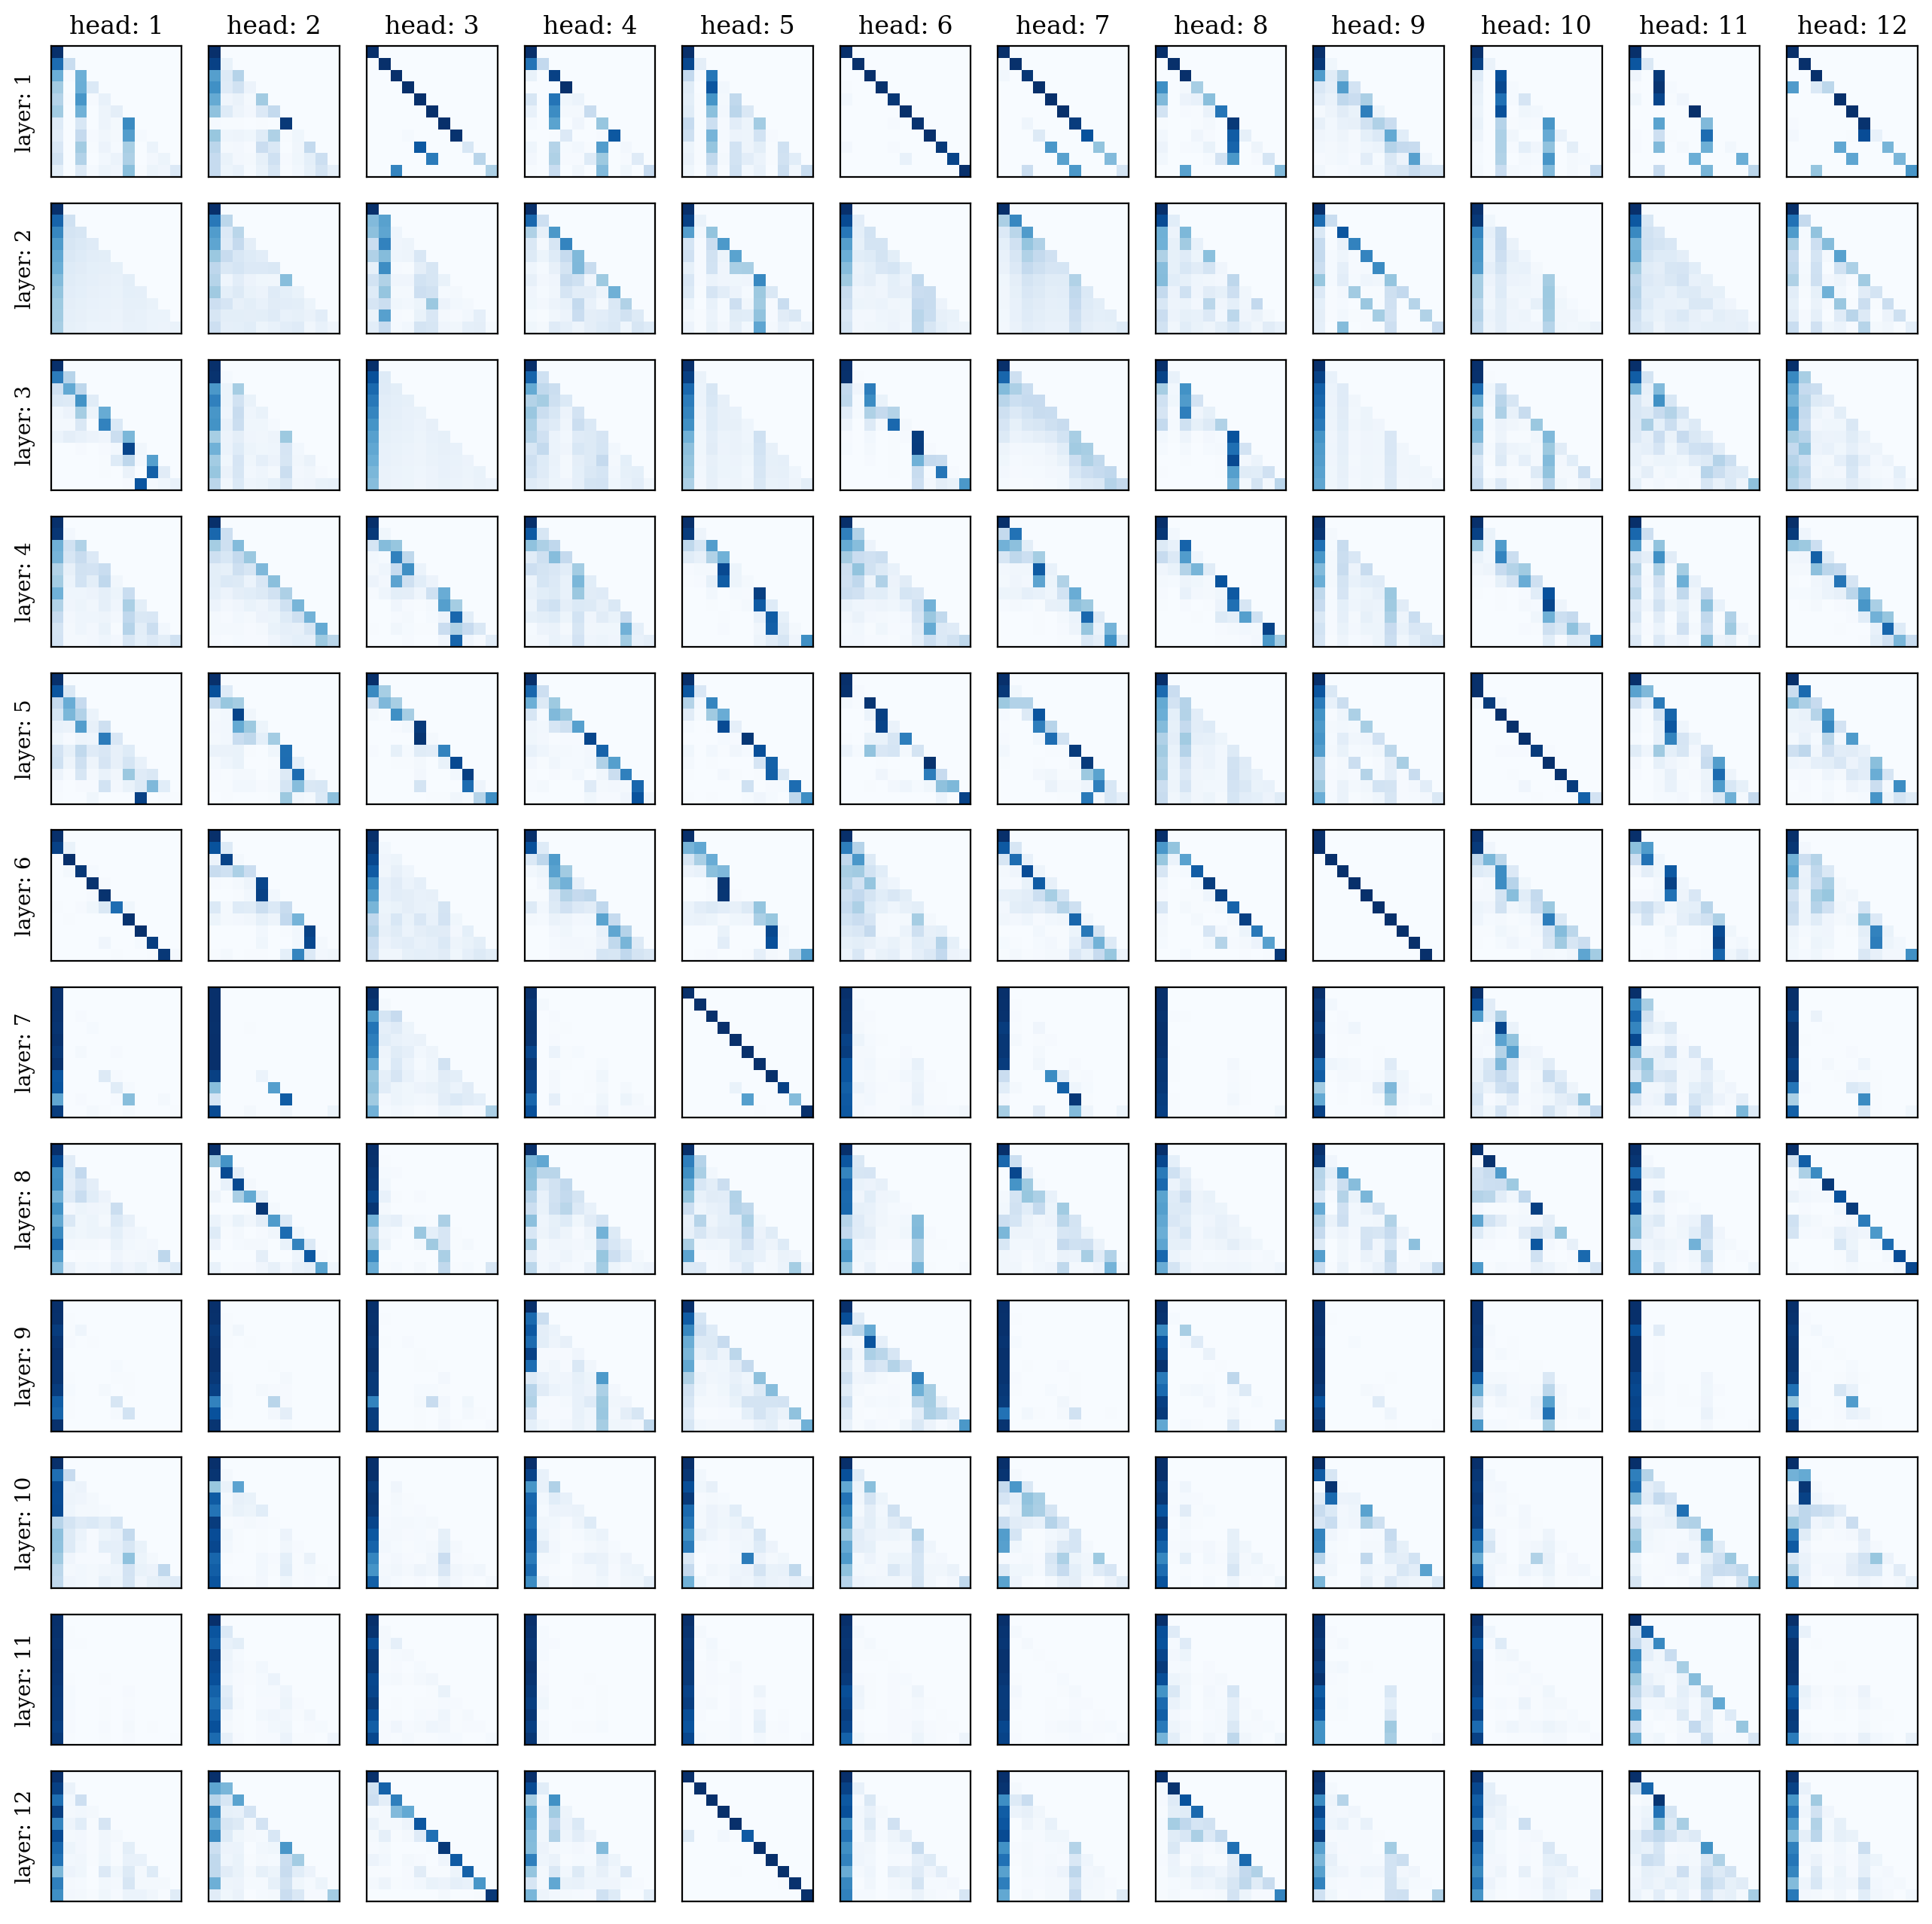
\includegraphics[width=\linewidth]{figures/gpt_neo_attn.png}
    \vspace{2mm}
    % 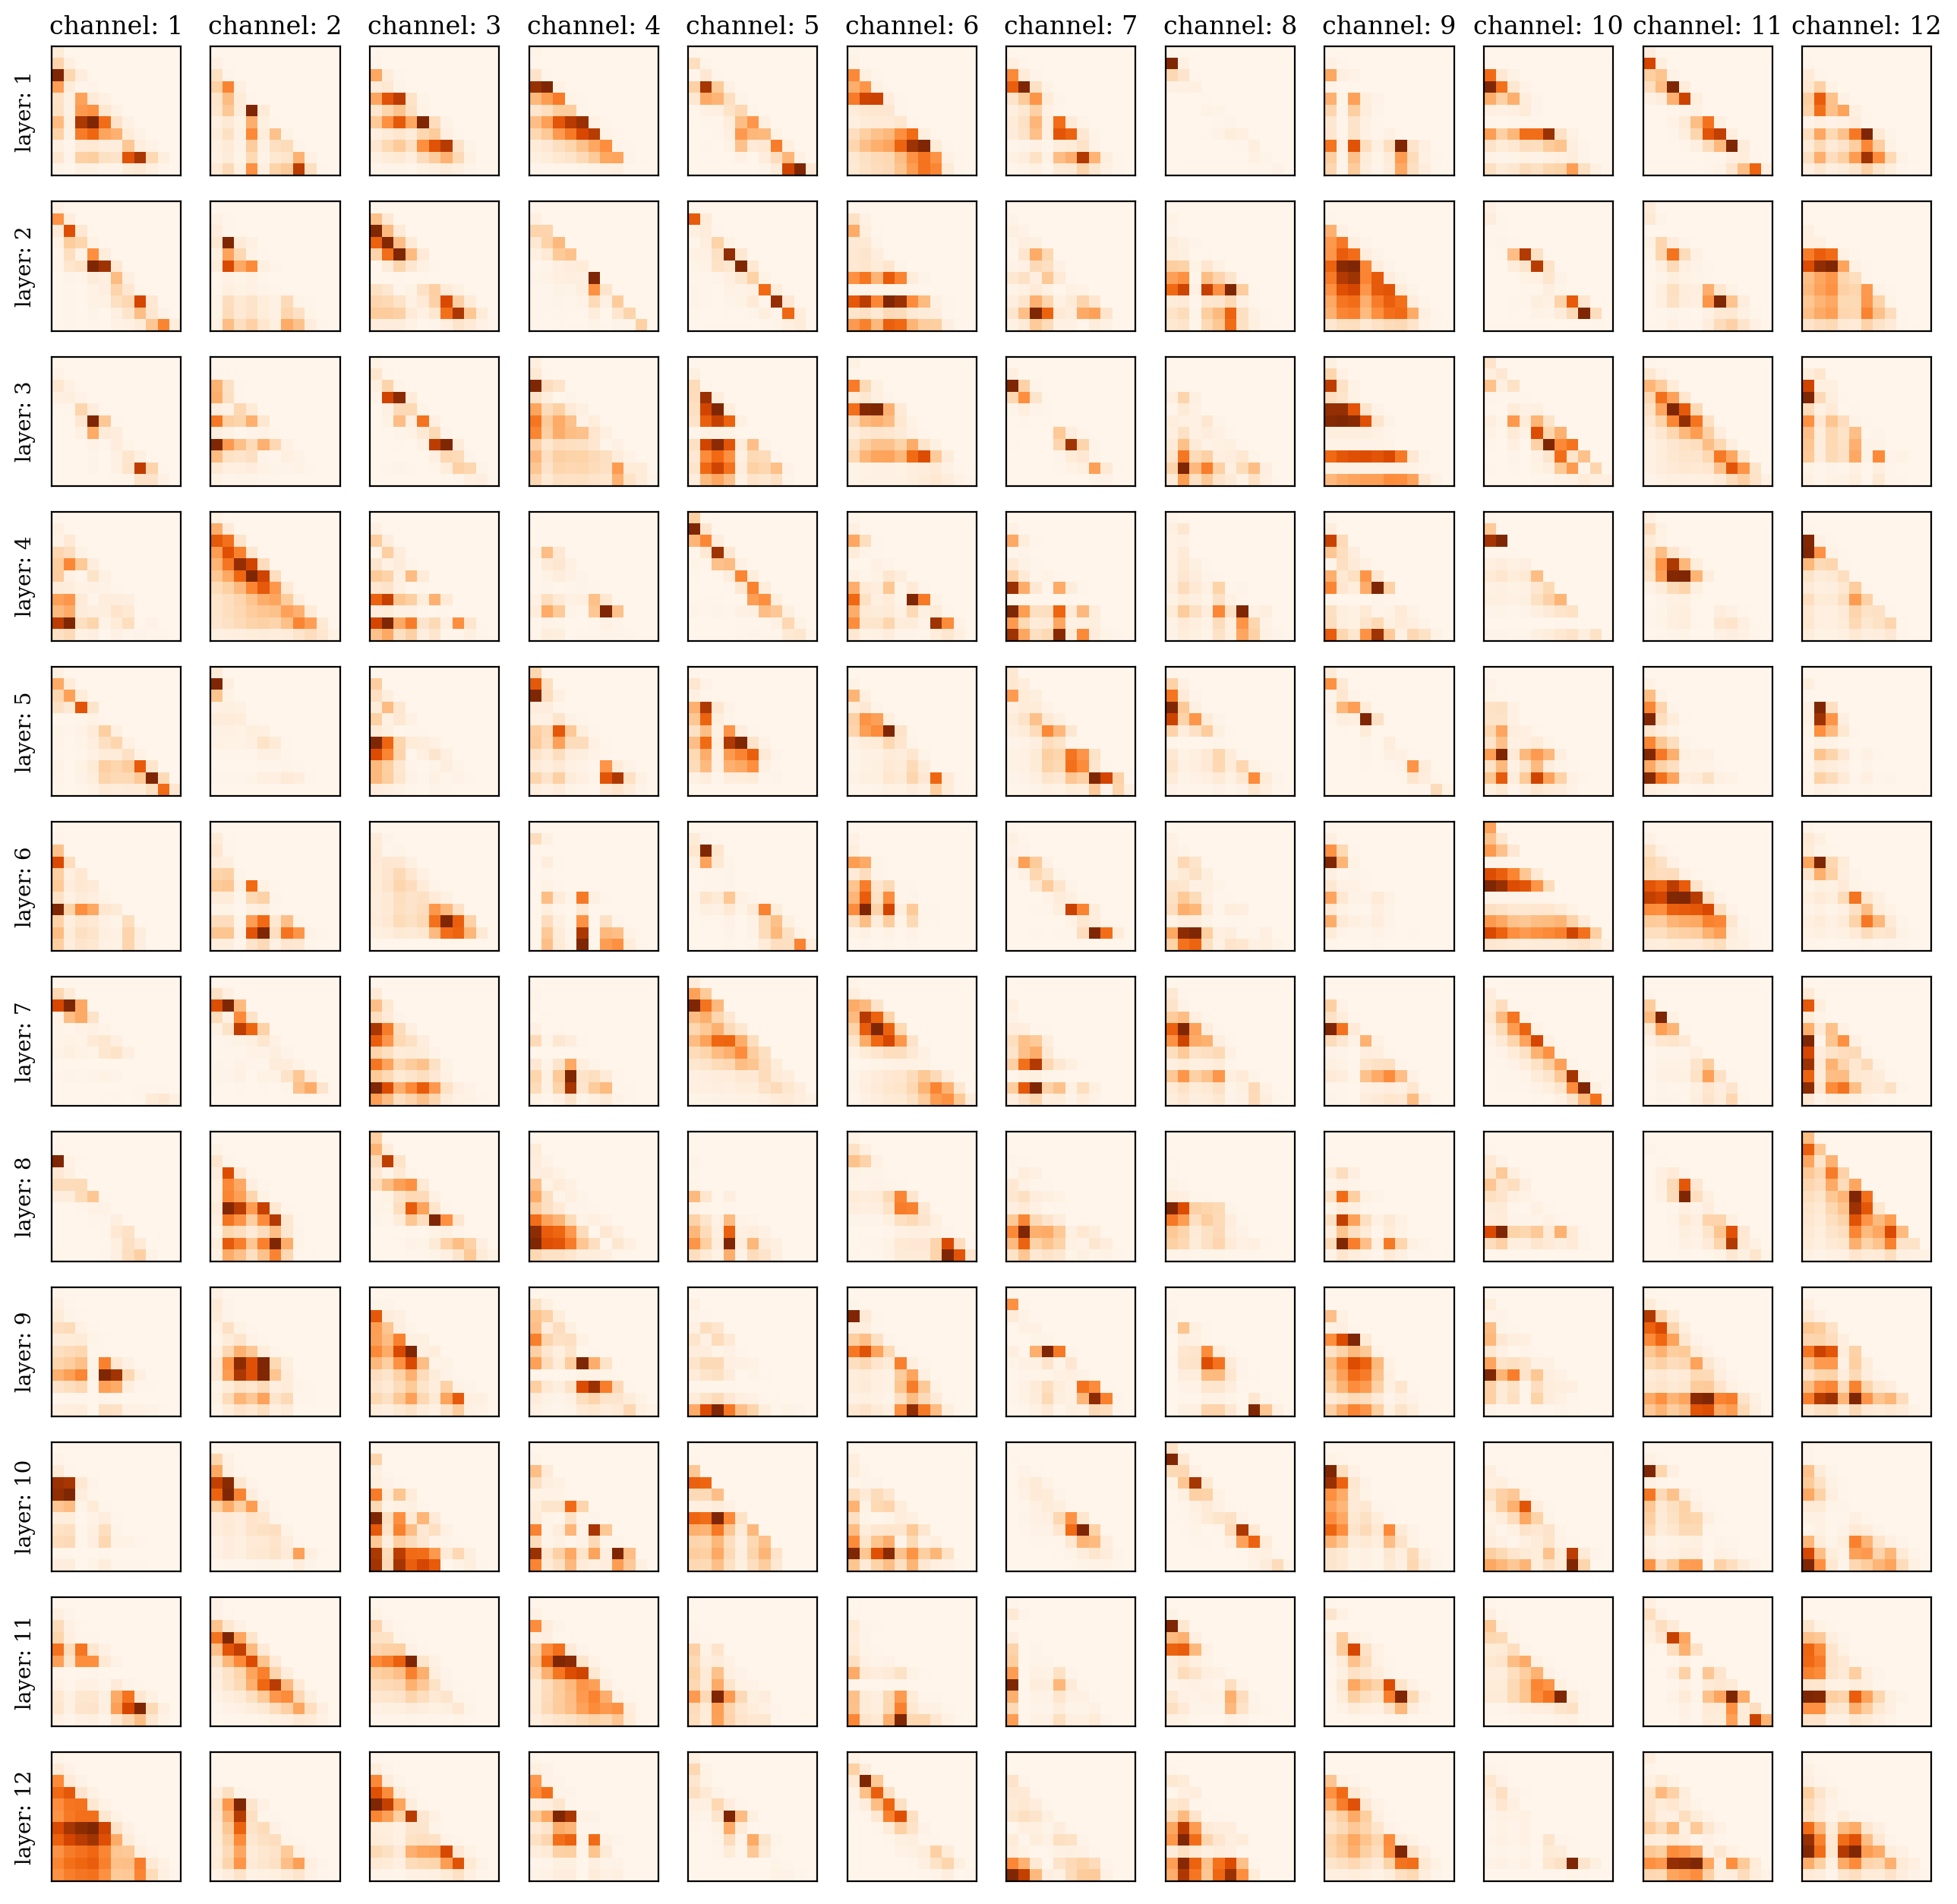
\includegraphics[width=0.6\linewidth]{figures/hyena_mats.png}
    %\caption{\textbf{[Top]}: Attention matrices from a GPTNeo small model. \textbf{[Bottom]}:  Hyena matrices from a {\sf Hyena} small (same model used for SuperGLUE downstream evaluations). "We use the test string "\textit{Attention is all you need. Attention is}". We note that {\sf Hyena} has a different data-controlled matrix for each \textit{channel} i.e. for each dimension in its width, since it does not use heads.}
    \caption{Attention matrices from a GPTNeo small model. "We use the test string "\textit{Attention is all you need. Attention is}".}
    \label{fig:comparisons_1}
\end{figure}
%
\begin{figure}
    \centering
    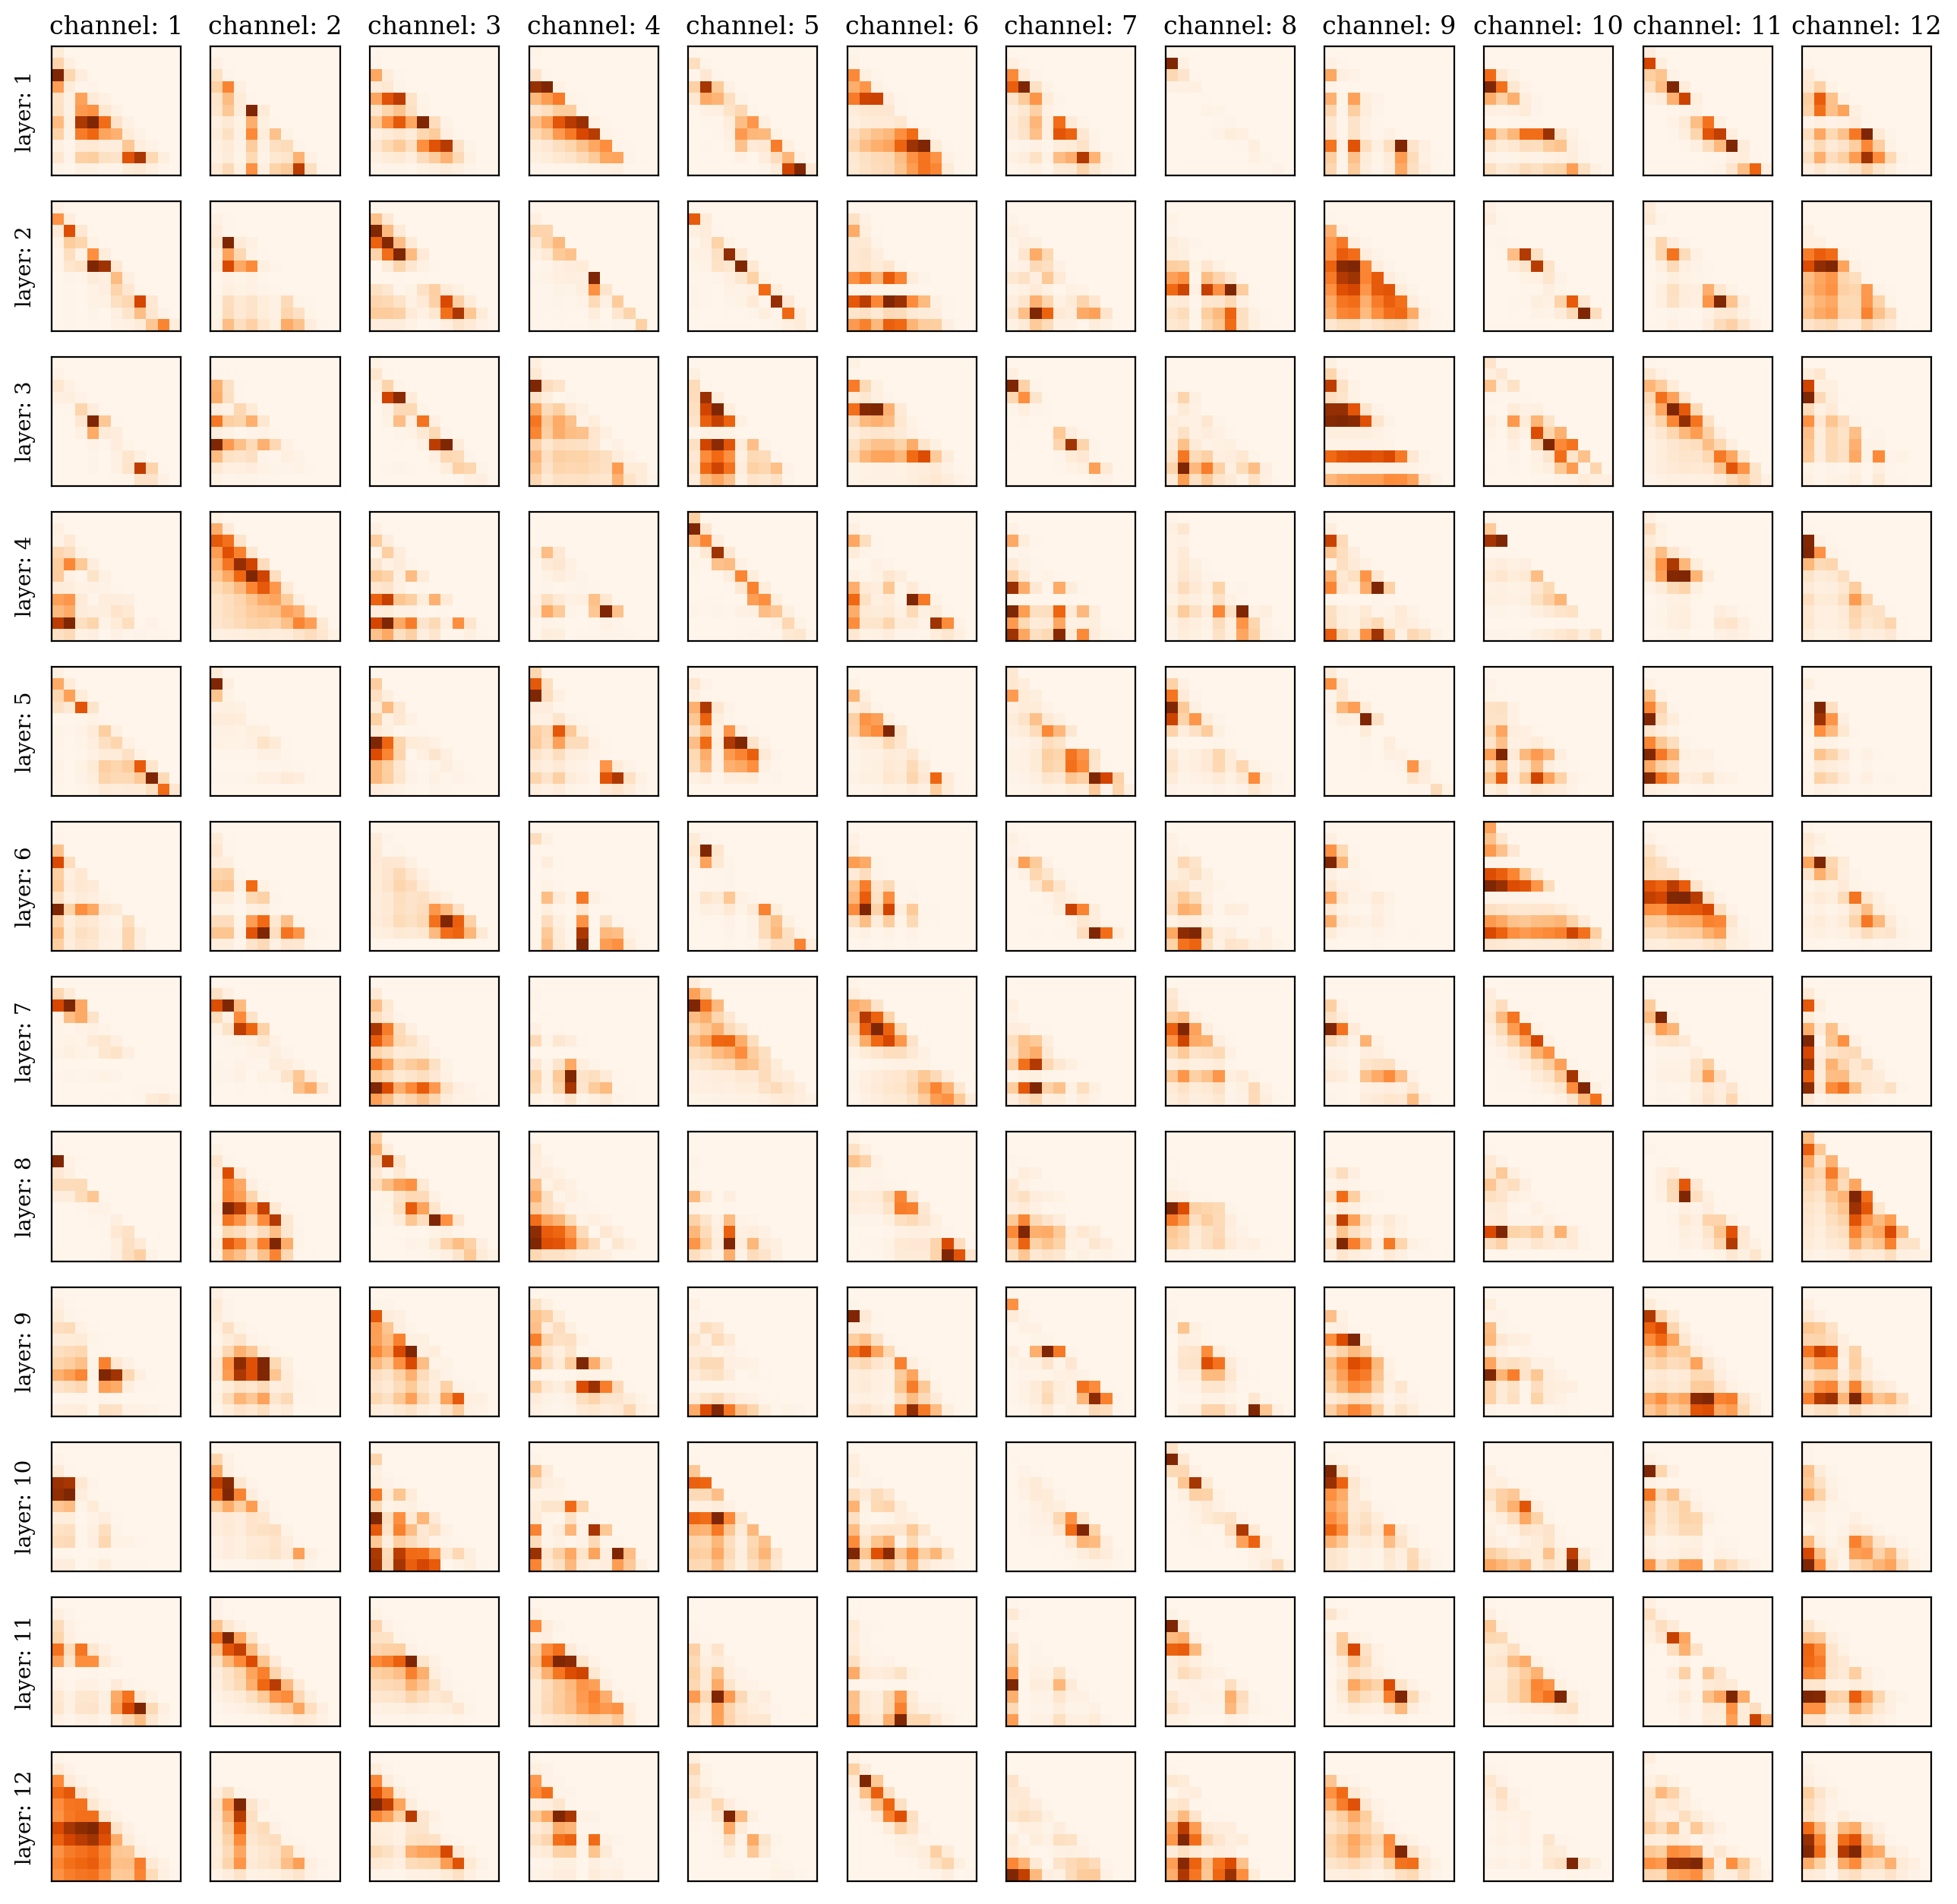
\includegraphics[width=\linewidth]{figures/hyena_mats.png}
    \caption{Hyena matrices from a {\sf Hyena} small (same model used for SuperGLUE downstream evaluations). "We use the test string "\textit{Attention is all you need. Attention is}". We note that {\sf Hyena} has a different data-controlled matrix for each \textit{channel} i.e. for each dimension in its width, since it does not use heads.}
    \label{fig:comparisons_2}
\end{figure}
%

\begin{figure}[h]
    \centering
    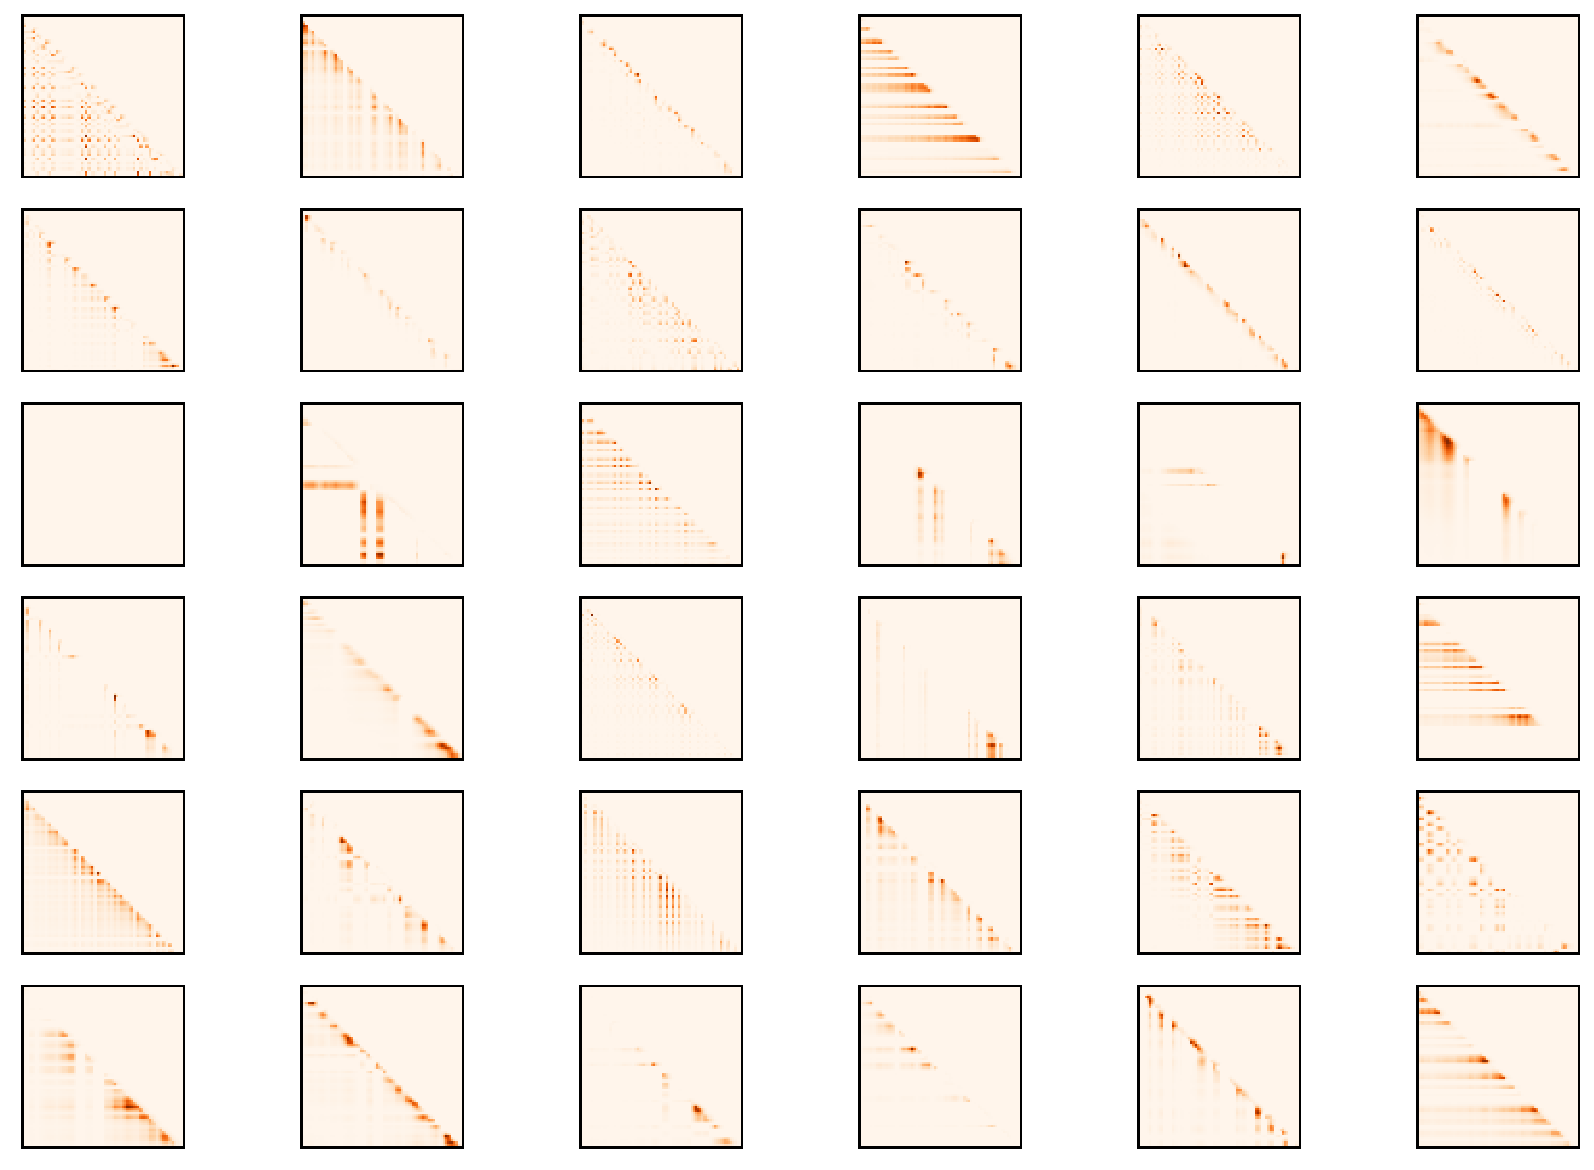
\includegraphics[width=\linewidth]{figures/hyena_doctor.pdf}
    \caption{Data-controlled ${\sf Hyena}$ matrices ($355$M model), activated by the string "\textit{When a doctor doctors a doctor, does the doctor doing the doctoring doctor as the doctor being doctored wants to be doctored or does the doctor doing the doctoring doctor as they want to doctor?}". Rows in the plot are matrices from different layers, columns are matrices from different channels. The operator shows characteristic patterns of attention matrices, without attention.}
    \label{fig:visu}
\end{figure}
\begin{figure}[h]
    \centering
    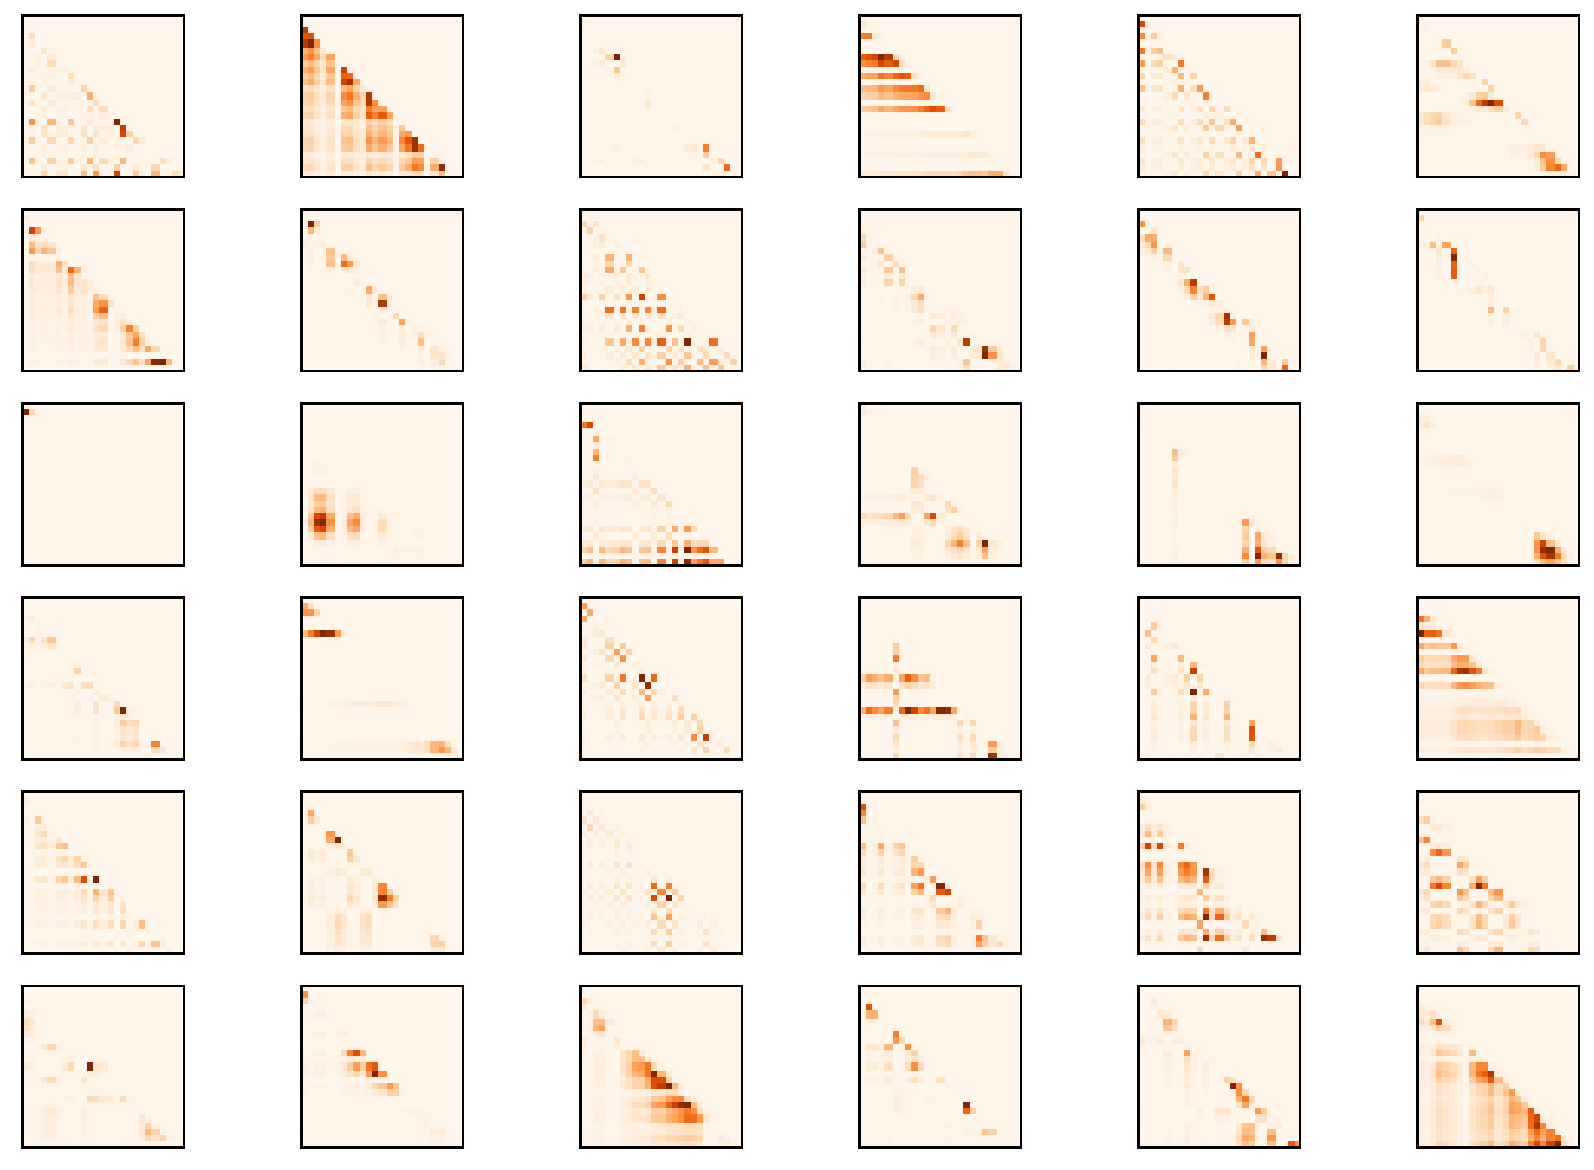
\includegraphics[width=\linewidth]{figures/hyena_dursley.pdf}
    \caption{Data-controlled ${\sf Hyena}$ matrices ($355$M model), activated by the string "\textit{Mrs. Dursley, Mr. Dursley, Dudley Dursley}", from \href{ttps://www.lesswrong.com/posts/j6s9H9SHrEhEfuJnq/causal-scrubbing-results-on-induction-heads}{\textit{Causal scrubbing: results on induction heads}}. Rows in the plot are matrices from different layers, columns are matrices from different channels.}
    \label{fig:visu2}
\end{figure}

\clearpage 

\subsection{Hyena Filters}

Figure \ref{fig:hyena_filters} provides a visualization of {\sf Hyena} long convolution filters at initialization and after training to completion on {\sc The Pile}. 

 We find a substantial performance difference (up to $5\%$ perplexity) between initialization schemes. If the filters at initialization are excessively smooth (see Appendix \ref{app:posemb} for a discussion of positional encoding and activation), the model finds a worse solution and takes longer to converge. Further, we observe initialization schemes that regularize filters towards typical filters learned at convergence to decrease performance. These observations are in line with performance gaps between convolution parametrization schemes discussed in main text and Appendix \ref{app:icl}. In particular, the performance improvements obtained via {\sf Hyena} filters could be due to easier optimization in the space of convolutional filters.


%
 At convergence, {\sf Hyena} learns a collection of lower-order filters with a similar structure, which can be exploited to further speed up inference after training. 

 
\begin{figure}
    \centering
    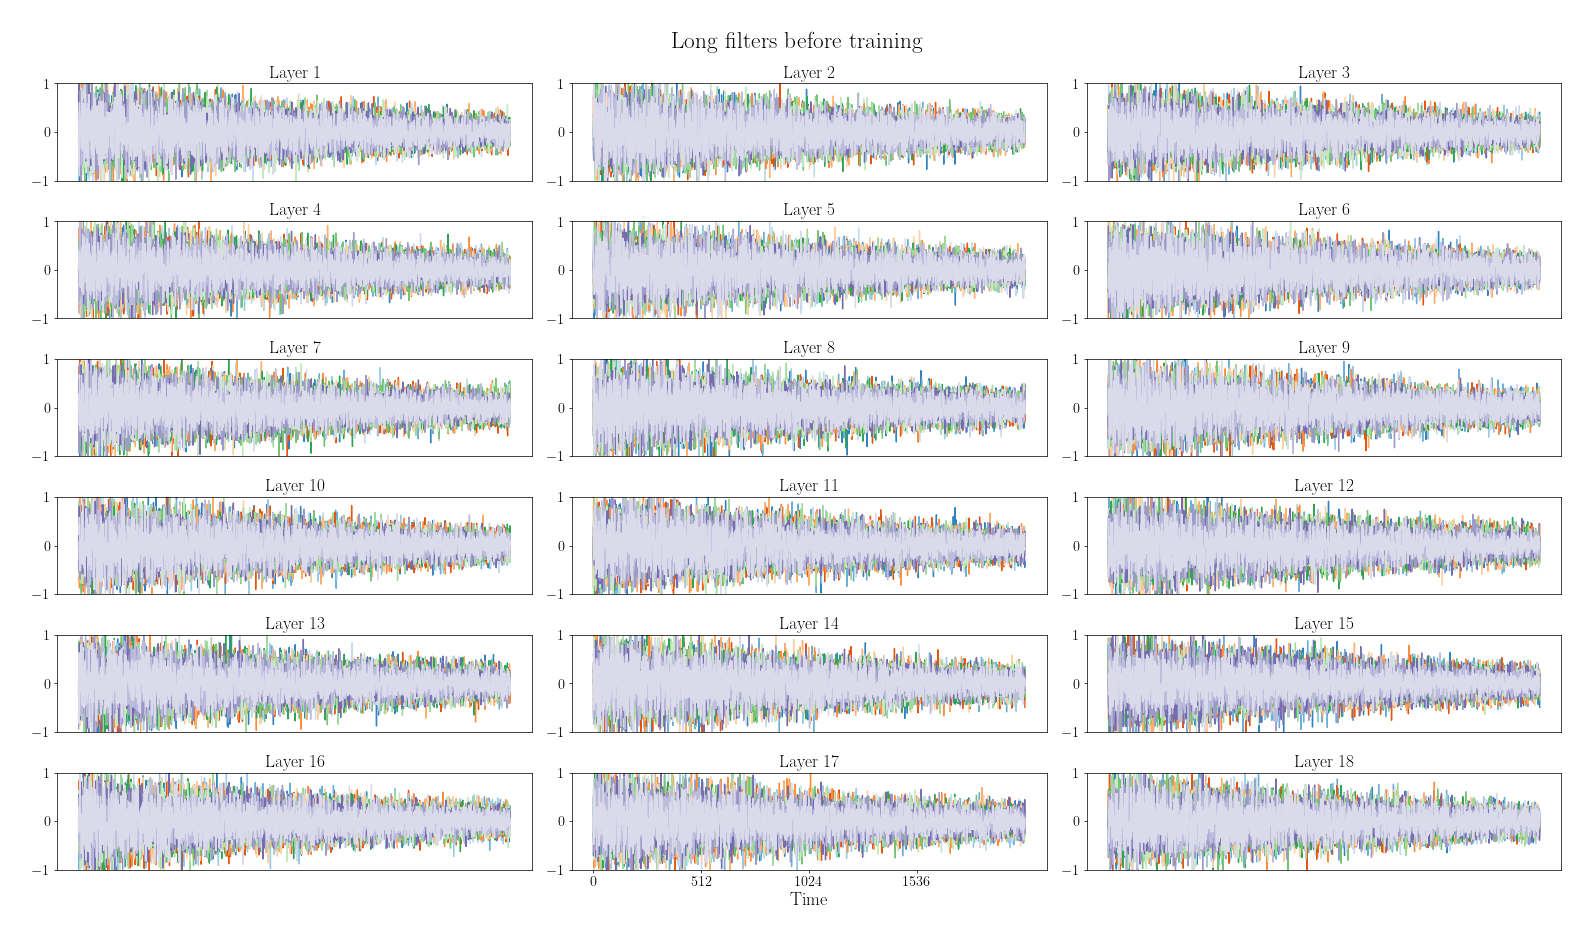
\includegraphics[width=0.99\linewidth]{figures/long_filters_init.png}
    \vspace{2mm}
    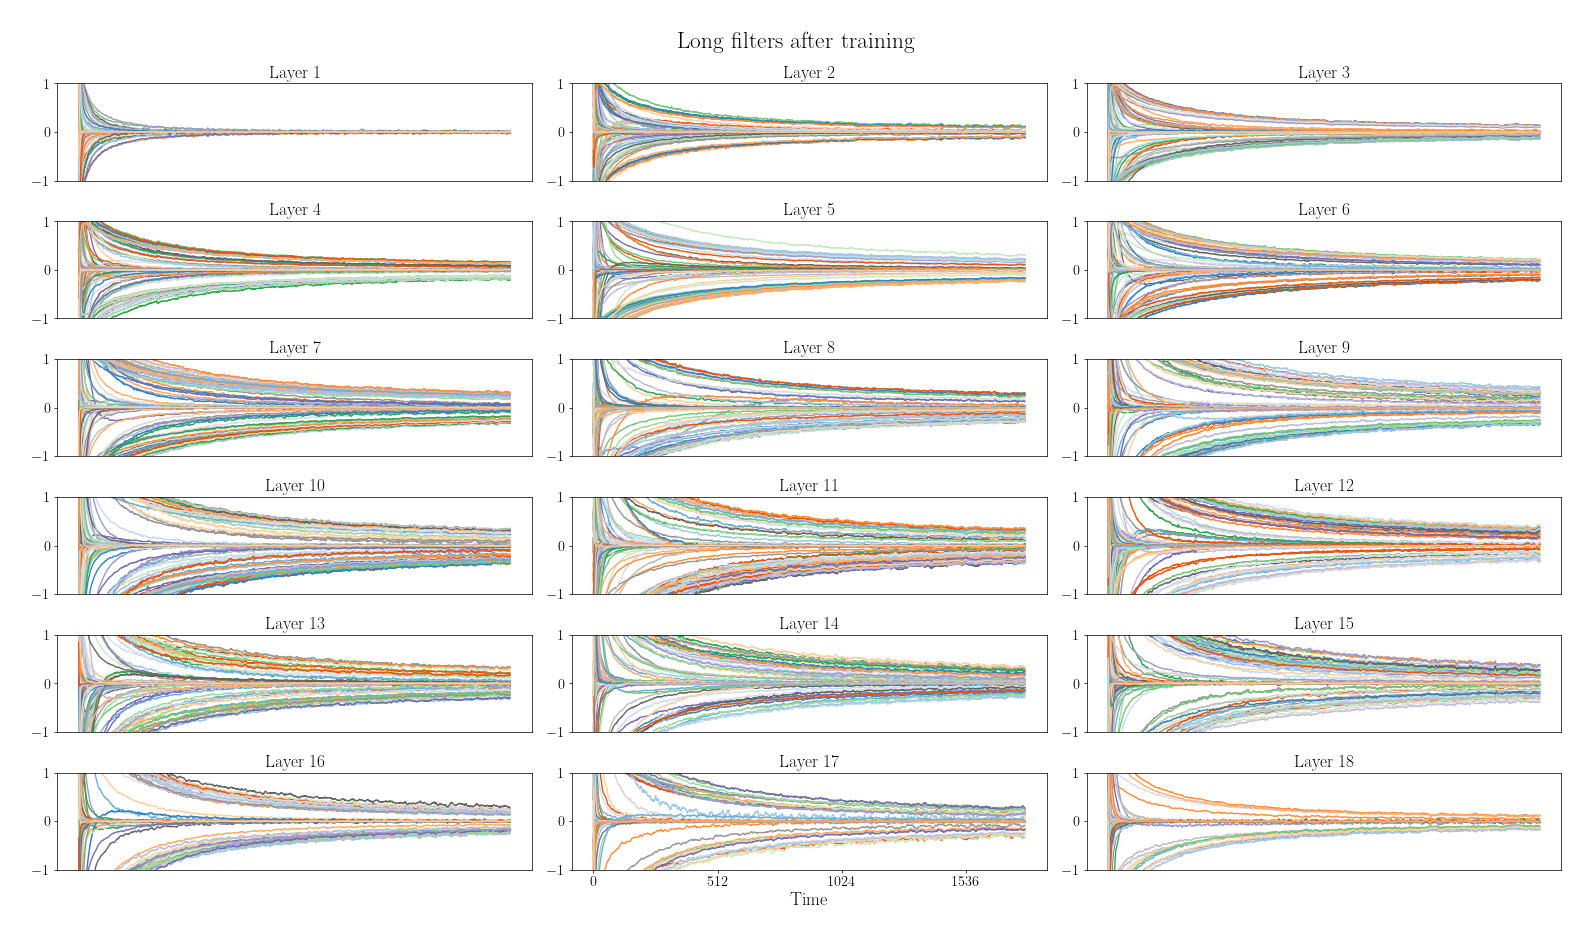
\includegraphics[width=0.99\linewidth]{figures/long_filters.png}
    \caption{\textbf{[Top]}: Long convolution {\sf Hyena} filters at initialization ($153$M parameters, $18$ layer model). \textbf{[Bottom]}: Filters after training for $130$ billion tokens on {\sc The Pile}.}
    \label{fig:hyena_filters}
\end{figure}

\subsection{Positional Encoding and Filters Initialization}\label{app:posemb}
%
The positional encoding chosen for the $\sf Hyena$ filters is a truncated complex exponential basis. Specifically, with $\rho_k(t) = e^{i2\pi kt/L}$ for $k=0,\dots K-1$, the positional encoding is defined as a map from $\R$ to $\R^{2K+1}$ such that
%
\[
    {\sf PositionalEncoding}(t) = 
    \begin{bmatrix}
        t&
        \mathfrak{R}[\rho_0](t)&
        \cdots&
        \mathfrak{R}[\rho_{K-1}](t)&
        \mathfrak{I}[\rho_0](t)&
        \cdots&
        \mathfrak{I}[\rho_{K-1}](t)
    \end{bmatrix}
\]
%
where $\mathfrak{R}[\cdot]$, $\mathfrak{I}[\cdot]$ denote the real and imaginary part of their argument, respectively. In the main text, we use $D_e = 2K + 1$ to denote the size of a positional encoding with $K$ features. The number of features of the positional encoding has an impact on the filter initialization and training performances. In particular, we show how $K$ leads to a preconditioning of the spectrum of the filter at initialization. Figures~\ref{fig:pos_enc_17_1},~\ref{fig:pos_enc_65_1},~\ref{fig:pos_enc_128_1} display the initialized filters (with no $\sf Window$ function) for different values of $K$ ($\{8, 32, 64\}$) for $L=128$ and frequency $\omega_a$ of sinusoidal activation $\sigma(\cdot) = \sin(\omega_a \cdot)$ set to 1. We notice how the choice of $K$ induces a bias in the modeled frequencies at initialization. Specifically the filters resemble low-pass filters with a cut-off frequency of approximatively $2K + 1$. 

This cut-off frequency is strongly related to the \textit{smoothness} of the filter; as previously mentioned, we empirically observe better training dynamics of filters initialized to be non-smooth, i.e. with a rich high-frequency content. While we can achieve good initializations by increasing $K$, this results in larger $\sf FFN$s (its input dimension is $2K + 1$, i.e. the number of positional encoding features) which come with a higher parameter count. A more efficient solution is to increase the frequency $\omega_a$ of the sinusoidal activation. Figure~\ref{fig:pos_enc_17_10} show how with $K=8$ we can cover the full spectrum simply by setting $\omega_a=10$. 

%
\begin{figure}
    \centering
    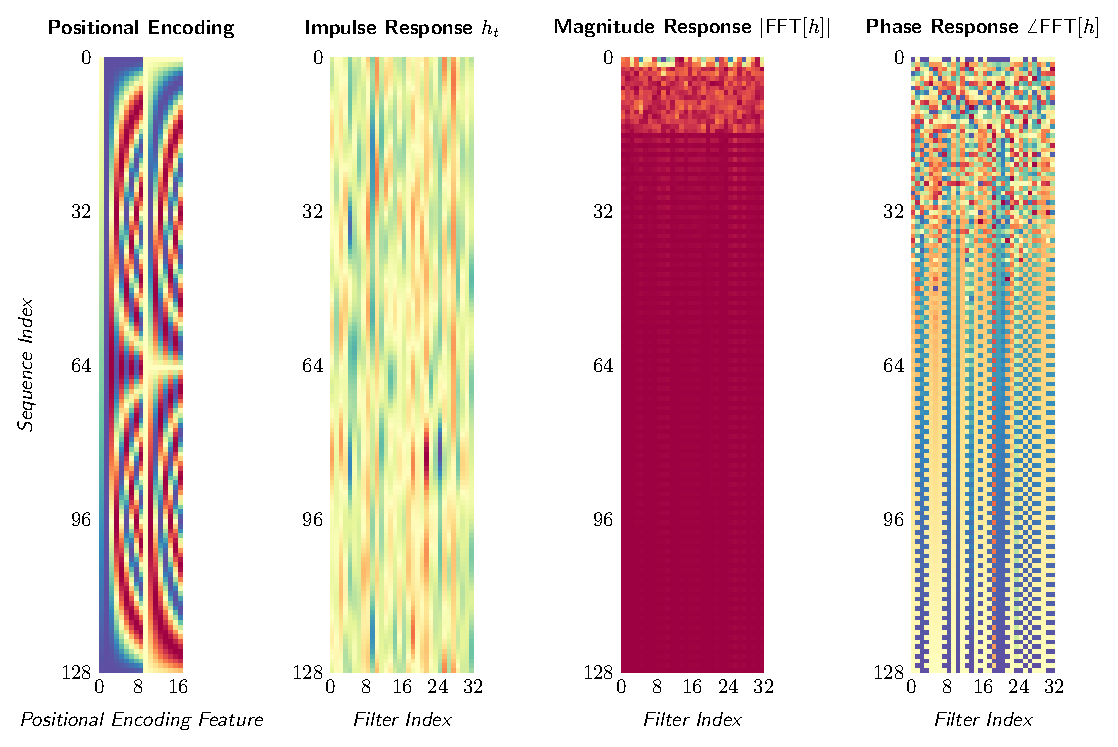
\includegraphics[width=.8\linewidth]{figures/pos_enc_17_sin_freq_1.pdf}
    \caption{$\sf Hyena$ filters at initialization with 17 positional encoding features $K=8$.}
    \label{fig:pos_enc_17_1}
\end{figure}
\begin{figure}
    \centering
    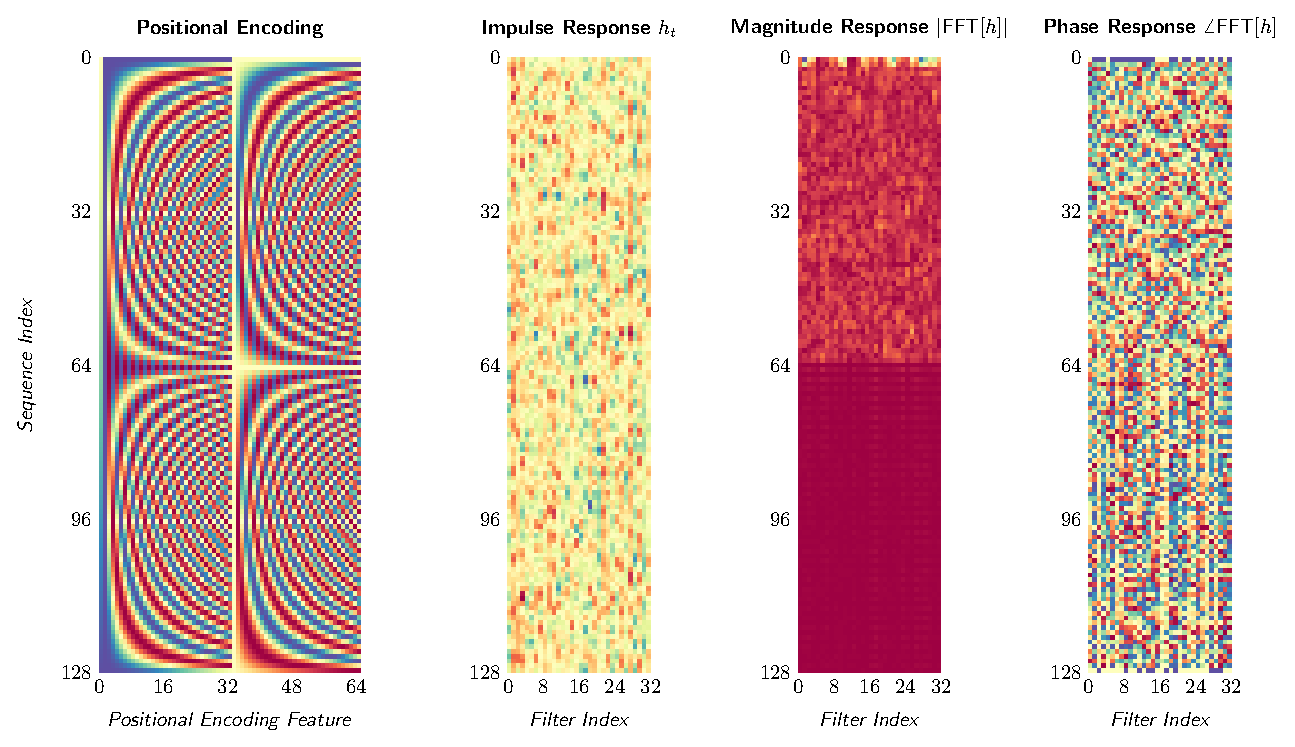
\includegraphics[width=.8\linewidth]{figures/pos_enc_65_sin_freq_1.pdf}
    \caption{$\sf Hyena$ filters at initialization with 65 positional encoding features $K=32$.}
    \label{fig:pos_enc_65_1}
\end{figure}
\begin{figure}
    \centering
    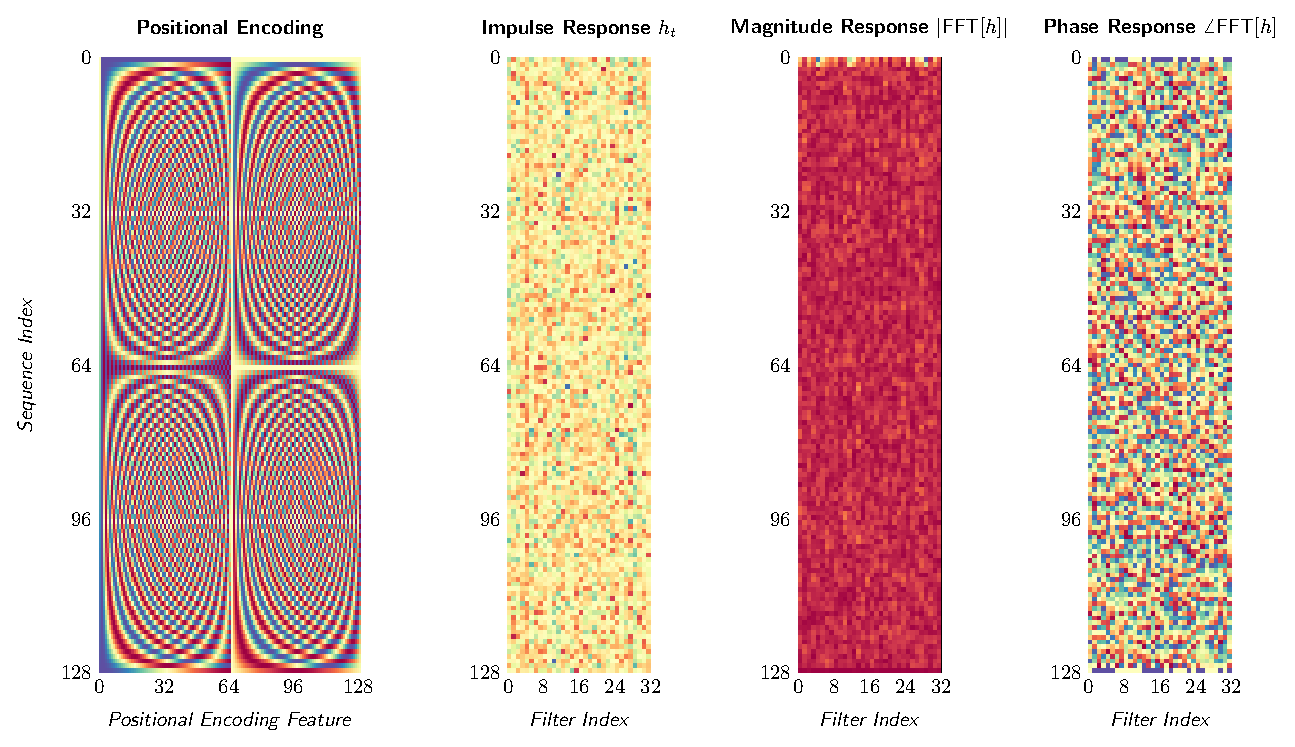
\includegraphics[width=.9\linewidth]{figures/pos_enc_129_sin_freq_1.pdf}
    \caption{$\sf Hyena$ filters at initialization with 65 positional encoding features $K=64$.}
    \label{fig:pos_enc_128_1}
\end{figure}
\begin{figure}
    \centering
    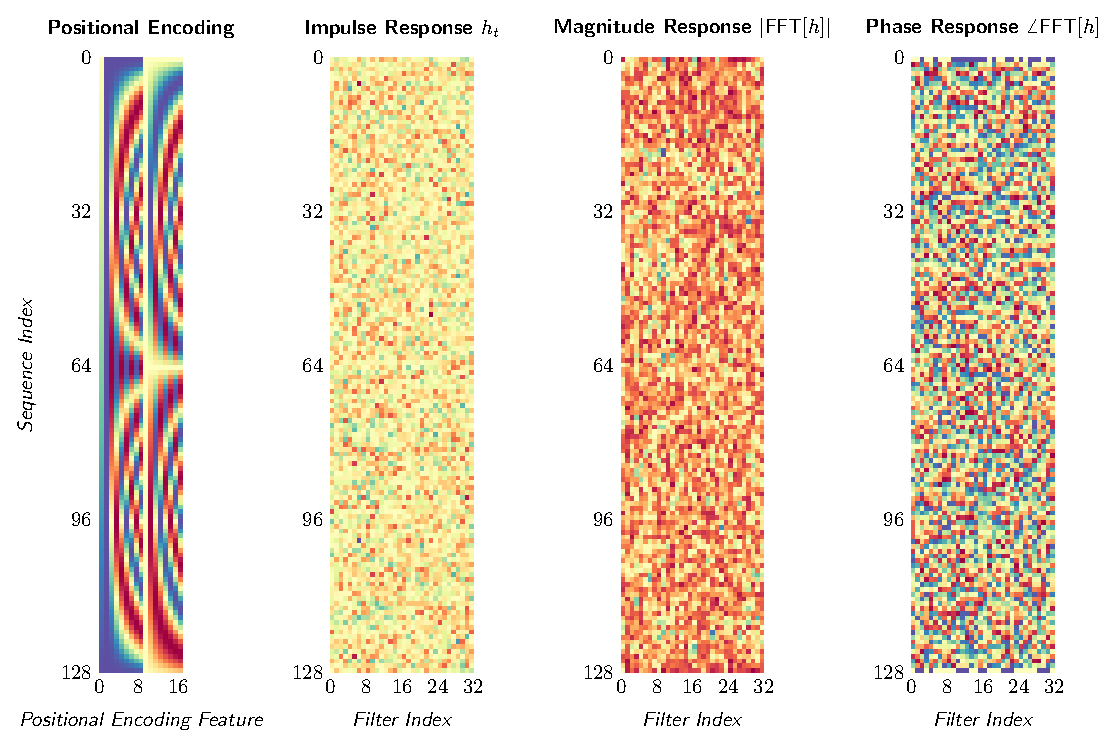
\includegraphics[width=.9\linewidth]{figures/pos_enc_17_sin_freq_10.pdf}
    \caption{$\sf Hyena$ filters at initialization with 17 positional encoding features $K=8$ and frequency of sinusodial activation set to 10.}
    \label{fig:pos_enc_17_10}
\end{figure}

\clearpage

\subsection{Downstream Examples}

\paragraph{MultiRC}
%

We report examples of downstream evaluation of small models on the MultiRC question-answering task. We report answers of small {\sf Hyena} (153M, trained for $130$B tokens on {\sc The Pile}) and the public checkpoint RWKV-v4 \citep{PENG_RWKV-LM_2021} ($169$M, trained for $332$B tokens on {\sc The Pile}). We select randomized examples with indices being powers of $2$.
%
Alignment of {\sf Hyena}'s responses to the task format is greatly improved by providing few-shot examples in the prompt, which may be a promising sign for larger models based on the proposed attention-free architecture.
Each example shows responses for specific examples in the validation set (example indices are listed at the beginning of each example).

\begin{tcolorbox}[sharp corners]
    {\tt MultiRC} index: 2, 4 \\ 
    
    \small {\tt \textbf{Passage:} What causes a change in motion? The application of a force. Any time an object changes motion, a force has been applied. In what ways can this happen? Force can cause an object at rest to start moving. Forces can cause objects to speed up or slow down. Forces can cause a moving object to stop. Forces can also cause a change in direction. In short, forces cause changes in motion. The moving object may change its speed, its direction, or both. We know that changes in motion require a force. We know that the size of the force determines the change in motion. How much an object's motion changes when a force is applied depends on two things. It depends on the strength of the force. It also depends on the object's mass. Think about some simple tasks you may regularly do. You may pick up a baseball. This requires only a very small force.} \\ 
    
    {\tt \textbf{Question:} Based on the previous passage, Would the mass of a baseball affect how much force you have to use to pick it up? Is "Less the mass, less the force applied" a correct answer?} \\

    {\tt \textbf{Answer:} Yes} \\ 

    {\tt {\color{red!80} RWKV zero-shot}: The mass of a baseball depends on the force applied. if the mass of the baseball is small, the force applied is small.}  \\ 

    {\tt {\color{blue!80}Hyena zero-shot}: Yes it is.}  \\

    {\tt {\color{red!80} RWKV few-shot}: The mass, less the force applied, is a more important force. it is the force that changes the mass of a baseball.} \\

    {\tt {\color{blue!80}Hyena few-shot}: Yes.} 

    \vspace{1cm}
    
     {\tt \textbf{Question:} Based on the previous passage, What do you apply to an object to make it move or stop? Is "Strength" a correct answer?} \\

    {\tt \textbf{Answer:} No} \\    

    {\tt {\color{red!80} RWKV zero-shot}: The force applied to the object is the force applied to the object.}  \\ 

    {\tt {\color{blue!80}Hyena zero-shot}: Yes.}  \\

    {\tt {\color{red!80} RWKV few-shot}: The force applied to a baseball is a force. it is a force that is applied to a baseball.} \\

    {\tt {\color{blue!80}Hyena few-shot}: Yes.} 
\end{tcolorbox}



\begin{tcolorbox}[sharp corners]
    {\tt MultiRC} index: 32, 64 \\ 
    
    \small {\tt \textbf{Passage:} The film opens with Sunita, a medical student, and her friends working on a project about the human brain. She wants to investigate the curious case of Sanjay Singhania, a notable city businessman, who is reported to have anterograde amnesia.  Her professor denies access to Sanjay's records as it is currently under criminal investigation.  Sunita, nonetheless, decides to investigate the matter herself.  Sanjay is introduced as he brutally murders a man. He takes a Polaroid picture of the man, and writes on it ``done''.  It is revealed that Sanjay has anterograde amnesia where he loses his memory every 15 minutes.  Sanjay uses a system of photographs, notes, and tattoos on his body to recover his memory after each cycle.  It is revealed that Sanjay is ultimately out to avenge the death of his sweetheart Kalpana, and that he is systematically killing the people who were responsible for it.  His main target is ``Ghajini'', a notable social personality in the city. Police Inspector Arjun Yadav, on the case of the serial murders, tracks Sanjay down to his flat and attacks and disables him. Yadav finds two diaries where Sanjay has chronicled the events of 2005 and 2006 . The film flashes back to 2005 as Yadav reads the diary. Sanjay Singhania is shown as the owner of the Air Voice mobile telephone company. In the course of his business, Sanjay sends his men to meet Kalpana, a struggling model, about putting up a billboard above her apartment. The owner of Kalpana's advertising firm misinterprets this as a romantic advance, and in view of a possible lucrative Air Voice ad campaign and other benefits, encourages Kalpana to accept the overture.} \\ 
    
    {\tt \textbf{Question:} Based on the previous passage, Why did Sanjay murder a man? Is "Sanjay" a correct answer?} \\

    {\tt \textbf{Answer:} Yes} \\ 

    {\tt {\color{red!80} RWKV zero-shot}: The answer is "Sanjay".}  \\ 

    {\tt {\color{blue!80}Hyena zero-shot}: The answer is}  \\

    {\tt {\color{red!80} RWKV few-shot}: The question is not about Sanjay's death.} \\

    {\tt {\color{blue!80}Hyena few-shot}: No.}  \\ 

    \vspace{1cm}

      {\tt \textbf{Question:} Based on the previous passage, Every 15 minutes, Sanjay goes through what process, Which frustrates his attempts to avenge the death of his sweetheart? Is "He forgets about facts" a correct answer?} \\

    {\tt \textbf{Answer:} Yes} \\    

    {\tt {\color{red!80} RWKV zero-shot}: Yes, it is a correct answer..}  \\ 

    {\tt {\color{blue!80}Hyena zero-shot}: The answer is.}  \\

    {\tt {\color{red!80} RWKV few-shot}: The answer is "yes".} \\

    {\tt {\color{blue!80}Hyena few-shot}: The answer is "yes.}    
\end{tcolorbox}

\begin{tcolorbox}[sharp corners]
    {\tt MultiRC} index: 128 \\ 
    
    \small {\tt \textbf{Passage:} In 1863, Alexander II re-convened the Diet of Finland and initiated several reforms increasing Finland\'s autonomy from Russia including establishment of its own currency, the markka. Liberation of business led to increased foreign investment and industrial development. Finland also got its first railways, separately established under Finnish administration. Finally, the elevation of Finnish from a language of the common people to a national language equal to Swedish opened opportunities for a larger proportion of the society. Alexander II is still regarded as "The Good Tsar" in Finland. These reforms could be seen as results of a genuine belief that reforms were easier to test in an underpopulated, homogeneous country, than in the whole of Russia. They may also be seen as a reward for the loyalty of its relatively western-oriented population during the Crimean War and during the Polish uprising. Encouraging Finnish nationalism and language can also be seen as an attempt to dilute ties with Sweden.} \\ 
    
    {\tt \textbf{Question:} Based on the previous passage, Alexander II is considered what in Finland since 1863? Is "The good tsar" a correct answer?} \\

    {\tt \textbf{Answer:} Yes} \\ 

    {\tt {\color{red!80} RWKV zero-shot}: The correct answer is "yes".}  \\ 

    {\tt {\color{blue!80}Hyena zero-shot}: Yes, the question is correct.}  \\

    {\tt {\color{red!80} RWKV few-shot}: The Finnish language is a language of the people.} \\

    {\tt {\color{blue!80}Hyena few-shot}: Yes.} 
\end{tcolorbox}


\begin{tcolorbox}[sharp corners]
    {\tt MultiRC} index: 1024 \\ 
    
    \small {\tt \textbf{Passage:} Einstein and Maric married in January 1903. In May 1904, the couple's first son, Hans Albert Einstein, was born in Bern, Switzerland. Their second son, Eduard, was born in Zurich in July 1910. In 1914, the couple separated; Einstein moved to Berlin and his wife remained in Zurich with their sons. They divorced on 14 February 1919, having lived apart for five years. Eduard, whom his father called "Tete" (for petit), had a breakdown at about age 20 and was diagnosed with schizophrenia. His mother cared for him and he was also committed to asylums for several periods, including full-time after her death. The marriage with Maric does not seem to have been very happy. In letters revealed in 2015, Einstein wrote to his early love, Marie Winteler, about his marriage and his still strong feelings for Marie. In 1910 he wrote to her that "I think of you in heartfelt love every spare minute and am so unhappy as only a man can be" while his wife was pregnant with their second child. Einstein spoke about a "misguided love" and a "missed life" regarding his love for Marie. Einstein married Elsa Lowenthal on 2 June 1919, after having had a relationship with her since 1912. She was a first cousin maternally and a second cousin paternally. In 1933, they emigrated to the United States. In 1935, Elsa Einstein was diagnosed with heart and kidney problems; she died in December 1936.} \\ 
    
    {\tt \textbf{Question:} Based on the previous passage, How much time passed, after Albert Einstein's father divorced his mother, that he re-married? Is "3 months and 18 days" a correct answer?} \\

    {\tt \textbf{Answer:} Yes} \\ 

    {\tt {\color{red!80} RWKV zero-shot}: Albert Einstein was born on 3 march 1916 in Gerlin, Germany. he was the son of a German doctor and a german woman.}  \\ 

    {\tt {\color{blue!80}Hyena zero-shot}: "3 months and 18 days"}  \\

    {\tt {\color{red!80} RWKV few-shot}: It is not a correct answer. The exact date is not known.} \\

    {\tt {\color{blue!80}Hyena few-shot}: Yes, according to the previous passage.} 
\end{tcolorbox}


%
\end{document}